%-------------------------------------------------------------------------------
% This file provides a skeleton ATLAS document
%-------------------------------------------------------------------------------
\documentclass[USenglish]{latex/atlasdoc}
% The language of the document must be set: usually UKenglish or USenglish
% british and american also work!
% Selected options:
%  atlasstyle=true|false Use ATLAS style for document (default)
%  coverpage             Create ATLAS draft cover page for collaboration circulation
%                        See atlas-draft-cover.tex for a list of variables that should be defined.
%  cernpreprint          Create front page for a CERN preprint
%                        See atlas-preprint-cover.tex for a list of variables that should be defined.
%  CONF                  The document is a CONF note (only useful together with coverpage)
%  PUB                   The document is a PUB note (only useful together with coverpage)
%  txfonts=true|false    Use txfonts rather than the default newtx - needed for arXiv submission
%  paper=a4|letter       Set paper size to A4 (default) or letter
%  maketitle=true|false  Run or do not run \maketitle from the class

%-------------------------------------------------------------------------------
% Extra packages:
\usepackage{latex/atlaspackage}
% Selected options:
%  biblatex=true|false   Use biblatex (default) or bibtex for the bibliography
%  backend=biber         Use the biber backend rather than bibtex
%  minimal               Minimal set of packages
%  default               Standard set of packages
%  full                  Full set of packages
% Style file with biblatex options for ATLAS documents
\usepackage{latex/atlasbiblatex}

% Package for creating list of authors and contributors to the analysis
\usepackage{latex/atlascontribute}

% Useful macros
\usepackage{latex/atlasphysics}
% See doc/atlas-physics.pdf for a list of the defined symbols
% Default options are
%   true:  journal, misc, particle, unit, xref
%   false: bsm, hion, math, process, other, texmf
% See the package for details on the options

% Files with references for use with biblatex
% Note that biber gives an error if it finds empty bib files
\addbibresource{TriggerProcessorDRR.bib}
\addbibresource{bibtex/bib/atlas-paper.bib}

% Paths for figures - do not forget the / at the end of the directory name
\graphicspath{{logos/}{figures/}}

% Add you own definitions here (file TriggerProcessorDRR-defs.sty)
\usepackage{TriggerProcessorDRR-defs}
\usepackage{maybemath}
\usepackage{booktabs}
\usepackage{comment}
\usepackage{titlesec}  % To create a \subsubsubsection
\usepackage{pdfpages}  % Adding PDF documents into the latex

%\setcounter{secnumdepth}{5} % Section depth to be numbered
%\setcounter{tocdepth}{5} % Table of contents depth

% Creating a new command \subsubsubsection
\titleclass{\subsubsubsection}{straight}[\subsection]
\newcounter{subsubsubsection}[subsubsection]
\renewcommand\thesubsubsubsection{\thesubsubsection.\arabic{subsubsubsection}}
%\renewcommand\theparagraph{\thesubsubsubsection.\arabic{paragraph}} % optional; useful if paragraphs are to be numbered

\titleformat{\subsubsubsection}
  {\normalfont\normalsize\bfseries}{\thesubsubsubsection}{1em}{}
\titlespacing*{\subsubsubsection}
{0pt}{3.25ex plus 1ex minus .2ex}{1.5ex plus .2ex}

\makeatletter
\renewcommand\@dotsep{1000}
\renewcommand\paragraph{\@startsection{paragraph}{5}{\z@}%
  {3.25ex \@plus1ex \@minus.2ex}%
  {-1em}%
  {\normalfont\normalsize\bfseries}}
\renewcommand\subparagraph{\@startsection{subparagraph}{6}{\parindent}%
  {3.25ex \@plus1ex \@minus .2ex}%
  {-1em}%
  {\normalfont\normalsize\bfseries}}
\def\toclevel@subsubsubsection{4}
\def\toclevel@paragraph{5}
\def\toclevel@paragraph{6}
\def\l@subsubsubsection{\@dottedtocline{4}{7em}{4em}}
\def\l@paragraph{\@dottedtocline{5}{10em}{5em}}
\def\l@subparagraph{\@dottedtocline{6}{14em}{6em}}
\makeatother

\setcounter{secnumdepth}{4}
\setcounter{tocdepth}{4}


%-------------------------------------------------------------------------------
% Generic document information
%-------------------------------------------------------------------------------

% Author and title for the PDF file
\hypersetup{pdftitle={ATLAS draft},pdfauthor={The NSW Trigger Processor Working Group}}
% Title, abstract and document
%-------------------------------------------------------------------------------
% This file contains the title, author and abstract.
% It also contains all relevant document numbers used by the different cover pages.
%-------------------------------------------------------------------------------

% Title
\AtlasTitle{Trigger Processor Design Review Report}

% Author - this does not work with revtex (add it after \begin{document})
\author{The NSW Trigger Processor Working Group}

% Authors and list of contributors to the analysis
% \AtlasAuthorContribute also adds the name to the author list
% Include package latex/atlascontribute to use this
% Use authblk package if there are multiple authors, which is included by latex/atlascontribute
% \usepackage{authblk}
% \renewcommand\Authands{, } % avoid ``. and'' for last author
% \renewcommand\Affilfont{\itshape\small} % affiliation formatting
% \AtlasAuthorContributor{Jo\~{a}o Guimar\~{a}es da Costa}{a}{Coordination, MM TP studies and testing}
% \AtlasAuthorContributor{Lorne Levinson}{b}{Coordination, sTGC TP firmware, algorithm and ancillary functions}
% \AtlasAuthorContributor{Samira Hassani}{c}{MM Trigger Algorithm}
% \AtlasAuthorContributor{Claude Guyot}{c}{MM Trigger Algorithm}
% \AtlasAuthorContributor{Philippe Schune}{c}{MM Trigger Algorithm}
% \AtlasAuthorContributor{Hevr\'{e} le Provost}{c}{MM Trigger Algorithm}

%% Names that can/should be added
%%Sorin Martoiu, Gabriel Stoicea, Michele Renda (IFIN-HH, Bucharest)

%\AtlasAuthorContributor{Third AtlasAuthorContributor}{a}{Author's contribution.}
% \AtlasContributor{Fourth AtlasContributor}{Contribution to the analysis.}
%\author[a]{First Author}
%\author[a]{Second Author}
%\author[b]{Third Author}
 % \affil[a]{Harvard University}
 % \affil[b]{Weizmann Institute}
 % \affil[c]{CEA Saclay}


% If a special author list should be indicated via a link use the following code:
% Include the two lines below if you do not use atlasstyle:
% \usepackage[marginal,hang]{footmisc}
% \setlength{\footnotemargin}{0.5em}
% Use the following lines in all cases:
% \usepackage{authblk}
% \author{The ATLAS Collaboration%
% \thanks{The full author list can be found at:\newline
%   \url{https://atlas.web.cern.ch/Atlas/PUBNOTES/ATL-PHYS-PUB-2014-007/authorlist.pdf}}
% }

% Date: if not given, uses current date
%\date{\today}

% Draft version:
% Should be 1.0 for the first circulation, and 2.0 for the second circulation.
% If given, adds draft version on front page, a 'DRAFT' box on top of each other page, 
% and line numbers.
% Comment or remove in final version.
%\AtlasVersion{0.3}

% ATLAS reference code, to help ATLAS members to locate the paper
%\AtlasRefCode{GROUP-2015-XX}

% ATLAS note number. Can be an COM, INT, PUB or CONF note
% \AtlasNote{ATLAS-CONF-2014-XXX}
% \AtlasNote{ATL-PHYS-PUB-2014-XXX}
% \AtlasNote{ATL-COM-PHYS-2014-XXX}

% CERN preprint number
% \PreprintIdNumber{CERN-PH-2014-XX}

% ATLAS date - arXiv submission; to be filled in by the Physics Office
% \AtlasDate{\today}

% arXiv identifier
% \arXivId{14XX.YYYY}

% HepData record
% \HepDataRecord{ZZZZZZZZ}

% Submission journal and final reference
% \AtlasJournal{Phys.\ Lett.\ B.}
% \AtlasJournalRef{\PLB 789 (2014) 123}
% \AtlasDOI{}

% Abstract - % directly after { is important for correct indentation
\AtlasAbstract{%
The trigger signals from both the small Thin Gap Chambers (sTGC) and the MicroMegas (MM) chambers will be processed by the New Small Wheel (NSW) Trigger Processor cards
located in USA15. The trigger algorithms will be implemented in conventional FPGAs and housed in ATCA crates. The two chamber-technologies will share the same hardware and, as much as possible, the same firmware. The output of the trigger processor will be sent to the new Sector Logic boards, to be combined with the Big Wheel trigger and define the final Level 1 trigger signal. This document describes the current status of the NSW Trigger Processor project.
}

%-------------------------------------------------------------------------------
% The following information is needed for the cover page. The commands are only defined
% if you use the coverpage option in atlasdoc or use the atlascover package
%-------------------------------------------------------------------------------

% List of supporting notes  (leave as null \AtlasCoverSupportingNote{} if you want to skip this option)
% \AtlasCoverSupportingNote{Short title note 1}{https://cds.cern.ch/record/XXXXXXX}
% \AtlasCoverSupportingNote{Short title note 2}{https://cds.cern.ch/record/YYYYYYY}
%
% OR (the 2nd option is deprecated, especially for CONF and PUB notes)
%
% Supporting material TWiki page  (leave as null \AtlasCoverTwikiURL{} if you want to skip this option)
% \AtlasCoverTwikiURL{https://twiki.cern.ch/twiki/bin/view/Atlas/WebHome}

% Comment deadline
% \AtlasCoverCommentsDeadline{DD Month 2014}

% Analysis team members -- Indicate the Contact Editors (usually two) by (*) after their name
% \AtlasCoverAnalysisTeam{Peter Analyser, Contact Editor~(*), Contact Editor2~(*), Alphonse Physicien}

% Editorial Board Members --- Indicate the Chair by a (*) after his/her name
% Give either all members at once (then they appear on one line), or separately
% \AtlasCoverEdBoardMember{EdBoard~Chair~(*), EB~Member~1, EB~Member~2, EB~Member~3}
% \AtlasCoverEdBoardMember{EdBoard~Chair~(*)}
% \AtlasCoverEdBoardMember{EB~Member~1}
% \AtlasCoverEdBoardMember{EB~Member~2}
% \AtlasCoverEdBoardMember{EB~Member~3}

% A PUB note has readers and not an EdBoard -- give their names here (one line or several entries)
% \AtlasCoverReaderMember{Reader~1, Reader~2}
% \AtlasCoverReaderMember{Reader~1}
% \AtlasCoverEdBoardMember{Reader~2}

% Editors egroup
% \AtlasCoverEgroupEditors{atlas-GROUP-2014-XX-editors@cern.ch}

% EdBoard egroup
% \AtlasCoverEgroupEdBoard{atlas-GROUP-2014-XX-editorial-board@cern.ch}



% Document in: 
%https://svnweb.cern.ch/cern/wsvn/NSWELX/TriggerProcessor/documentation/DesignReviewFeb2015
%-------------------------------------------------------------------------------
% Content
%-------------------------------------------------------------------------------
\begin{document}

%\maketitle
\tableofcontents
\newpage

% List of contributors - print here or after the Bibliography
%\AtlasPrintContribute{0.3}


%-------------------------------------------------------------------------------
\section{Introduction}
\label{sec:intro}

This document presents the status of the New Small Wheel (NSW) Trigger Processor (TP) project and it is the main source of information for the ATLAS Design Review.
Information about the whole New Small Wheel detector system can be found in the New Small Wheel Technical Design Report\,\cite{NSWTDR}.
The Trigger Processor specifications are presented in Section\,\ref{sec:specs}.
These include a description of the interfaces to the two NSW trigger detectors (Micromegas, \MM, and small Thin Gap Chambers, \stgc),
of the interface to the muon end-cap Sector Logic and of the ancillary functionality of the Trigger Processor.
Section\,\ref{sec:algorithms} presents the trigger algorithms under consideration for both detector technologies,
including studies of the corresponding expected trigger performance and information regarding trigger duplicate handling.
The two options for the Trigger Processor hardware platforms are briefly introduced in Section~\ref{sec:hardware-platforms}, including a specification comparison and the criteria for a decision, with
further details provided in Refs.\,\cite{hardware-LAr-Carrier,hardware-LAr-OTC,hardware-SRS-Carrier,hardware-SRS-Mezz}.
The plans for testing the Trigger Processor hardware and firmware are presented in Section\,\ref{sec:testing},
followed by a brief discussion on the compatibility of the project with \PhaseTwo.
The document concludes with a concise overview of the project organization in Section\,\ref{sec:organization}.
%, including the schedule and responsibilities.
%Finally, the fiber plant is presented in Appendix~\ref{app:specs-fibers}.

\subsection{Overview of the NSW trigger}
\label{sec:Overview}

The main goal of the NSW trigger is to provide additional information to the muon Level-1 trigger (L1) in the \endcap region $1.0<|\eta|<2.4$, in order to dramatically reduce fake triggers arising from particles that are not high-\pt muons originating in the interaction point (IP).
A major source of fake triggers is low energy particles, mainly protons, generated in the material located between the Small Wheel and the end-cap middle station, the Big Wheel (BW).
As shown in Figure\,\ref{fig:NSW-Z}, these particles can cross the end-cap trigger chambers at an angle similar to that of real high \pt muons.
The NSW trigger signal is based on track segments produced online by the small Thin Gap Chambers (\stgc) and Micromegas chambers (\MM) comprising the NSW detectors.
These candidate track segments are input to the new Sector Logic (SL) that uses the information to corroborate trigger candidates from the BW TGC chambers.
The sector logic sends Level-1 trigger candidates to the ATLAS Muon Central Trigger system.

\begin{figure}[htb]
  \centering
  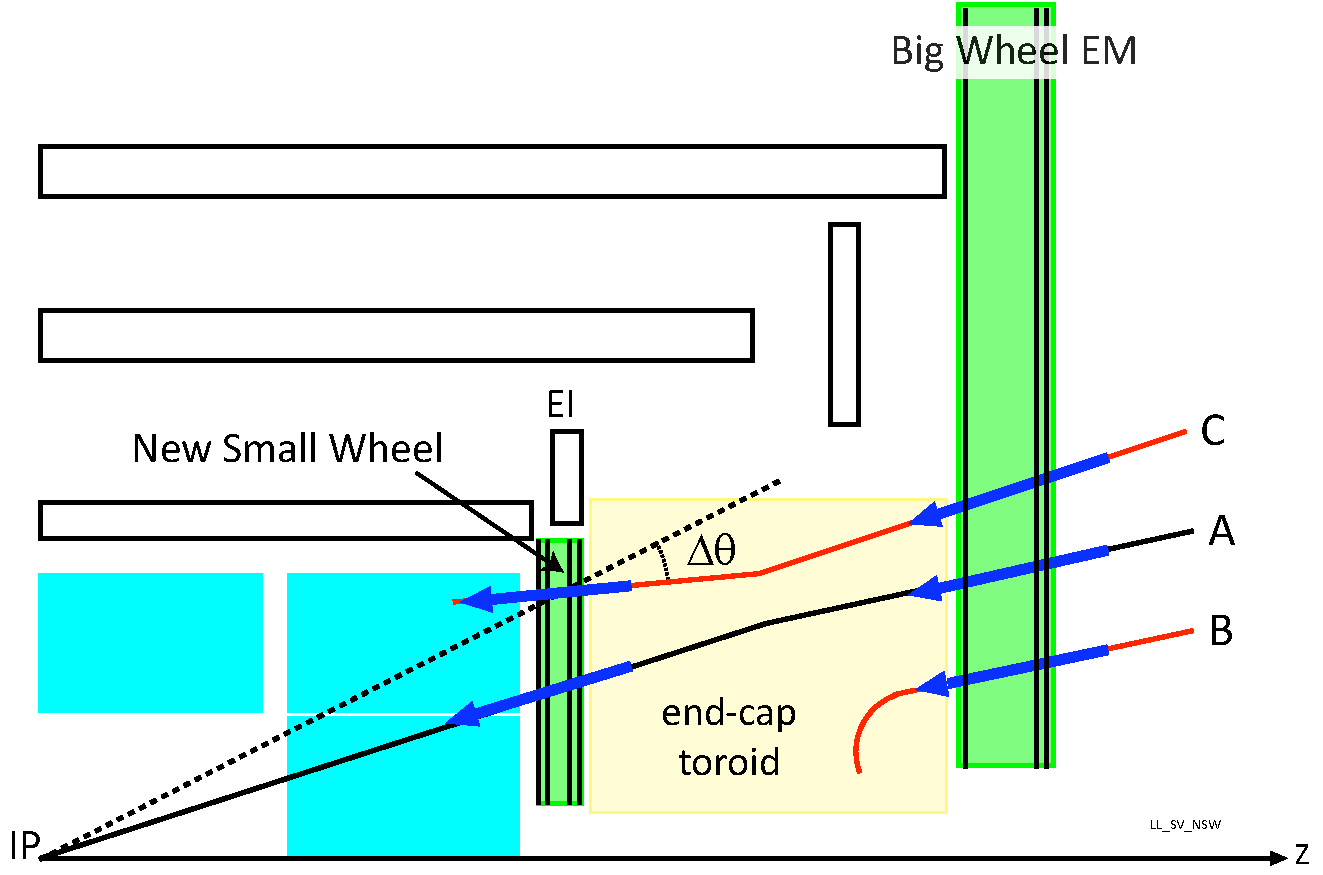
\includegraphics[width=0.6\textwidth]{figures/LL_SV_NSW.pdf}
%  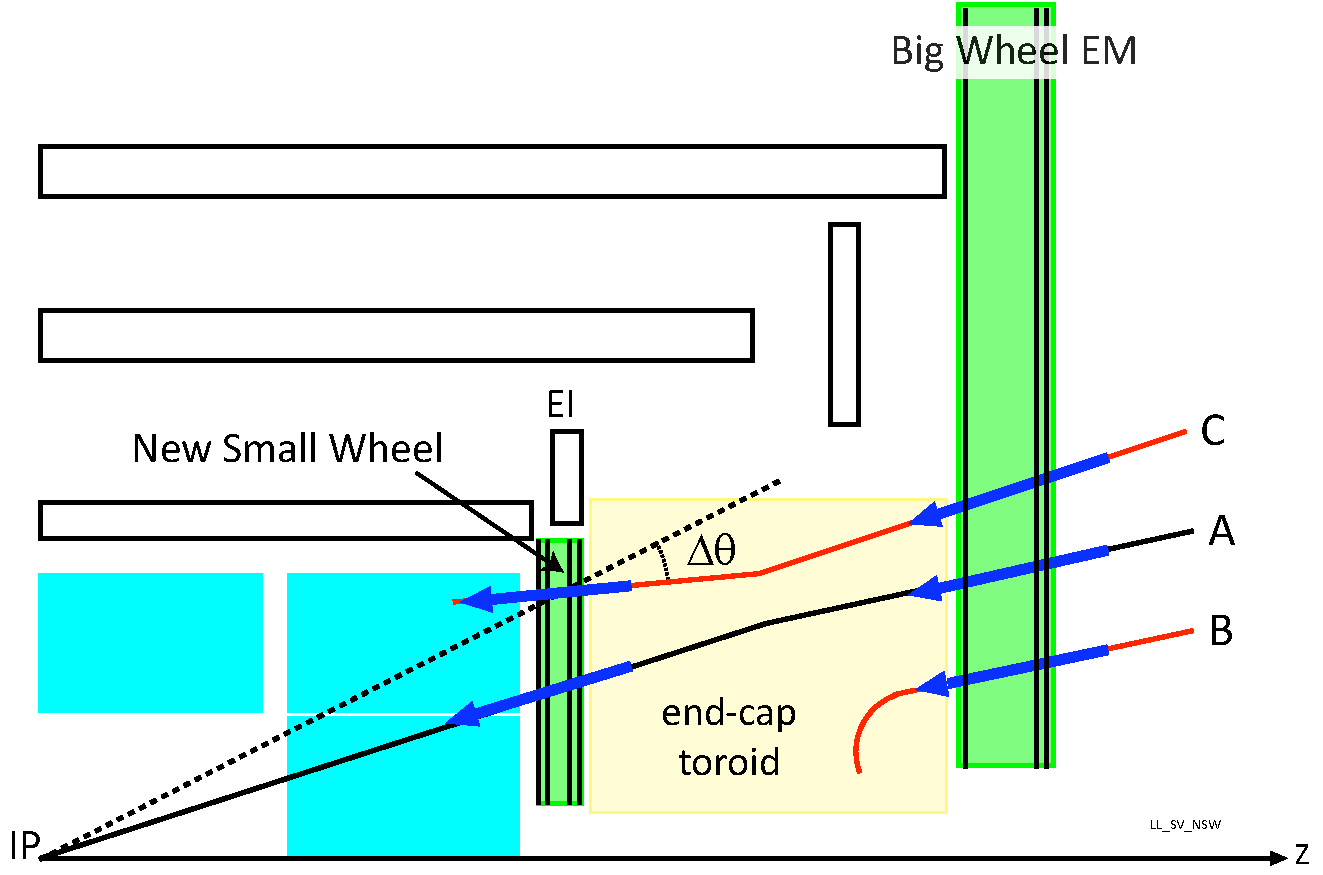
\includegraphics[trim=4cm 1.0cm 6.5cm 1.0cm, clip=true, width=0.6\textwidth]{figures/LL_SV_NSW.pdf}
  \caption{\small Schematic of the muon \endcap trigger. The existing Big Wheel trigger accepts all three tracks shown. With the addition of the NSW to the muon end-cap trigger, only track `A', the desired track, which is confirmed by both the Big Wheel and the NSW, will be accepted. Track `B' will be rejected because the NSW does not find a track coming from the interaction that matches the Big Wheel candidate. Track `C' will be rejected because the NSW track does not point to the interaction point (IP).
  The NSW logic restricts $\Delta\theta$ to a value consistent with the track to have originated from the IP.}
  \label{fig:NSW-Z}
\end{figure}

%\subsection{System layout and definitions}

\subsection{System granularity and terminology}
\label{sec:SystemLayout}

The \endcap trigger system operates independently on each detector \endcap (side A and side C).
Several other factors define the granularity of the \endcap trigger system.
The following recalls the terminology and boundary conditions of the overall \endcap trigger system:

\begin{itemize}
\item A {\bf New Small Wheel sector} comprises \sector of a wheel (i.e.\ one \endcap). Each wheel has eight large and eight small sectors. The detector and trigger sectors are coincidental.
\item The {\bf Big Wheel trigger detector} (BW-TGC) has 12 detector sectors per wheel.
Each sector is further divided into trigger sectors, four trigger sections per detector sector in the region at larger radius (\endcap region) and two trigger sectors in the region at smaller radius (forward region). This segmentation results in a total of 48 trigger sectors in the \endcap (larger radius) region and 24 trigger sectors in the forward region.
\item A {\bf Sector Logic board} serves two adjacent BW-TGC trigger sectors. For each side (A/C), there are 24 SL boards for the BW-TGC \endcap region and 12 SL boards for the BW-TGC forward region.
\item A SL board receives data from at most three NSW sectors.
\item For the NSW Trigger Processor, there is one {\bf FPGA} per detector technology (\MM or \stgc) per NSW sector. (\MM) and \stgc information is processed by separate algorithms in separate FPGAs. Depending on the hardware platform chosen, the two FPGAs will be located in the same mezzanine card (SRS option) or on two separate mezzanine cards (LAr option).
\item A {\bf NSW Trigger Processor ATCA board} (corresponding to two NSW sectors) contains the mezzanine cards (two or four depending on the hardware platform ultimately chosen) to serve a NSW octant.
\item One NSW trigger sector needs to deliver data to up to seven SL boards. The maximum fan-out of seven is needed for large NSW sectors, due to the overlap with the BW trigger sectors when multiple scattering, misalignments and magnetic field deformations are taken into account.
\end{itemize}


\subsection{Requirements and Limitations}
\label{sec:RequirementLimitations}

The main requirement for the NSW trigger is to provide track vector candidates from the NSW detectors to be matched to track segments from the BW.
The angular resolution on the NSW track vector candidates should be of 1\,mrad. In the data-taking period immediately after the installation of the NSW, during the Long Shutdown\,2 (LS2), the BW trigger granularity is limited to an angular resolution of 3\,mrad or larger. During the Long Shutdown\,3 (LS3), new BW trigger electronics and a new MDT Level-1 trigger will be deployed, allowing for 1\,mrad angular resolution in the BW.

\paragraph{Matching resolution requirements}
The NSW measures the radial coordinates in two planes, the azimuthal coordinate, $\phi$, and the angle, $\Delta\theta$, of track segments inside the wheel, i.e.\ before the end-cap toroid. $\Delta\theta$ is the angle of the segment with respect to an ‘infinite momentum track’, i.e.\ a line from the IP to the segment’s radial position in the NSW. The radial coordinate is measured by high-precision strips in both detectors. For the sTGC, $\phi$ is determined by the triggering tower of sTGC pads, and for the MM, by small angle stereo strips. The angle $\Delta\theta$ is to be measured to an accuracy close to 1\,mrad. The NSW trigger logic will rejects track segments with $\Delta\theta > \pm (7-15)$\,mrad (the final value will be determined from future studies).
The corroboration with the BW trigger is done by projecting the ‘infinite momentum track’ through the $R-\phi$ point of the segment in the NSW onto the BW’s $R-\phi$ array of Regions-of-Interest (RoI).
This matching requires the NSW trigger candidates to have:
\begin{itemize}\itemsep-6pt
\item $\phi$-resolution of 20\,mrad
\item $\eta$-resolution of 0.005
\end{itemize}
The angle $\Delta\theta$ is passed to the Sector Logic but is not used in the \PhaseOne trigger decision.

\paragraph{Simulation limitations}
The trigger model in the Athena simulation of both the sTGC and the MM trigger is not complete. A simulation of the correlated backgrounds is also needed. The following studies are particularly urgent:
\begin{itemize}\itemsep-4pt
\item Probability of finding track segments as a function of radius, in particular the probability for more than four candidates, in either \MM or \stgc, and for a total of eight candidates when duplicates are removed.
\item The $\phi$-resolution needed for matching to the BW RoI’s
\item Effects due to misalignment within the NSW and between the NSW and the BW
\end{itemize}



%-------------------------------------------------------------------------------

%-------------------------------------------------------------------------------
\section{Trigger Processor Specifications}
\label{sec:specs}
The context diagram in Figure~\ref{fig:TrigProcContext} shows the different interfaces to the NSW Trigger Processor
and the signal flow through the trigger system.
The NSW Trigger Processor is implemented in FPGAs on mezzanine cards of an ATCA carrier card.
One NSW sector (16~per end-cap wheel) is implemented on one FPGA (Xilinx Virtex~7 XC7VX690T).
Input and output fibers connect directly to the mezzanine cards.
Some services are on the carrier card which has an Ethernet connection.
The plan for the fiber connections from the front ends to the readout and trigger processors in USA-15 is shown in Appendix~\ref{app:specs-fibers}.

\begin{figure}[h]
	\centering
	%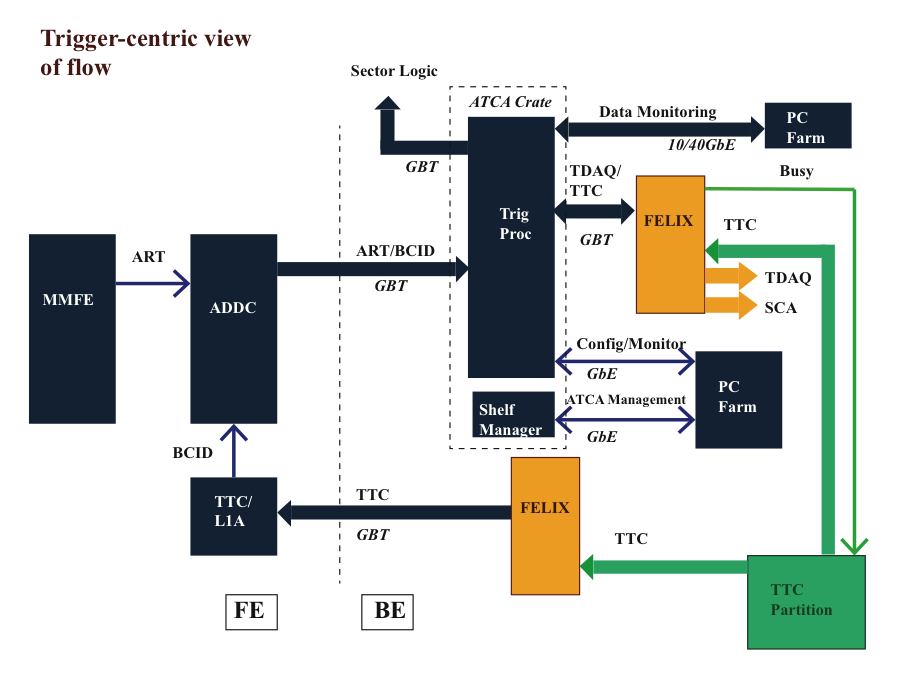
\includegraphics[width=0.8\textwidth]{specs/MMTriggerProcessorConfiguration}
	%\caption{Configuration relevant to the MM Trigger Processor.}
	%\label{fig:MMTriggerConfiguration}
	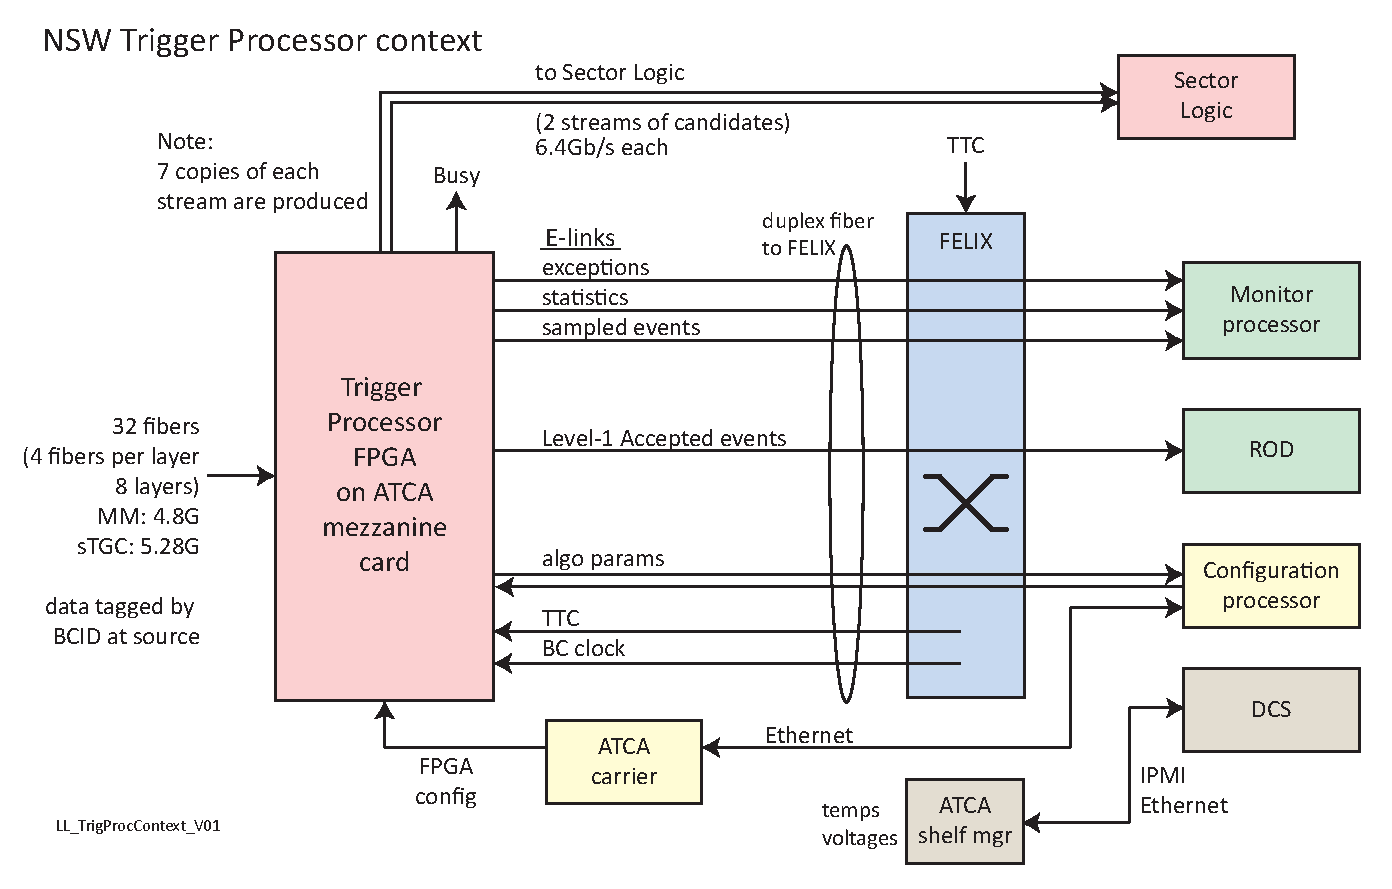
\includegraphics[width=0.97\textwidth]{figures/LL_TrigProcContext_V01.pdf}
	\caption{Trigger Processor context diagram}
	\label{fig:TrigProcContext}
\end{figure}

\vspace{-15pt}
\paragraph{Mezzanine card connections}
\begin{itemize}\itemsep-4pt\vspace{-5pt}
\item 32 input fibers from ADDC (MM) or Router (sTGC)
\item Several output fibers to the Sector Logic
\item An output fiber to FELIX which carries the following data flows on different E-links:
    \begin{itemize}\itemsep-6pt\vspace{-4pt}
    \item Level-1 Accept event readout
    \item Exception messages
    \item Statistics
    \item Sampled events
    \item Algorithm parameters
    \item TTC and BC clock
    \end{itemize}
\end{itemize}

\vspace{-15pt}
\paragraph{Services via the ATCA carrier}
\begin{itemize}\itemsep-4pt\vspace{-5pt}
\item Configuration of the FPGA itself via Ethernet
\item Temperature and voltage monitoring to DCS via Shelf Manager Ethernet
\end{itemize}

%Should the Trigger Processor FPGA become excessively utilized for the trigger algorithms,
%it is possible to move some of the non-algorithm logic to the FPGA on the carrier board.


\subsection{Trigger Processor Latency}
\label{sec:latency}

The trigger signal delivery time to the MuCTPI has to happen within 57~Bunch Crossings (BCs) (an increase of 3.5~BCs from the \PhaseZero system).
The New Sector Logic requires 16~BCs from the time it receives the trigger signal from the NSW and BW until it delivers it to the MuCTPI (5 BCs for serializer/deserializer,
9~BCs for trigger processing, and 2~BCs for transmission via fiber).
This leaves 43~BCs (1075~ns) for the full NSW trigger processing chain (including 2~BCs to merge the MM and sTGC trigger streams and time for the signal transmission to the Sector Logic).

The latency of the current design of the NSW trigger chain is at the
boundary of the required value, leaving no contingency.
It is therefore imperative to keep the latency as low as possible at
every step of the chain, including at the Trigger Processor.
The TP latency estimation is given in Table\,\ref{tab:latency} for both chamber technologies.
The accounting includes the input/output serializers, the trigger algorithm, the transmission time to the Sector Logic,
and the algorithm that merges the \MM and \stgc streams. The merging is currently planned to occur in the \stgc FPGA.

\begin{table}[htbp]
\centering
\begin{tabular}{l|cc|cc|l}
%\hline\hline
%\toprule
\toprule
    &\multicolumn{2}{c|}{sTGC} & \multicolumn{2}{c|}{MM} & \\
                                    & min   & max   & min  & max    &  Notes           \\
                                    & (ns)  & (ns)  & (ns) & (ns)   &                  \\
\midrule
Input deserializer (Rx)             & 40    & 40    & 44    & 44    &   \\
Trigger algorithm                   & 56    & 56    & 56    & 56    & 320\,MHz clock  \\
Stream merging algorithm            & 25    & 50    & --    & --    & Assigned to sTGC \\
Re-synch to 320 MHz clock           & 0     & 3.1   & 0     & 3.1   & $45^{\circ}$ phase chosen to  \\
\ \ driving output serializer       &       &       &       &       & \ \ \ best match pipeline length \\
Output to Sector Logic              & 25    & 30    & 25    & 30    & Deserializer on Sector Logic \\
\ \ serializer (Tx only)            &       &       &       &       & \ \ \ latency budget  \\
Fiber to Sector Logic               & 20    & 25    & 20    & 25    & 4-5\,m fiber @ 5\,ns/m  \\
\midrule
Total                               & 166   & 204.1 & 145   & 158.1 &     \\
\bottomrule
%\bottomrule
\end{tabular}
\caption{Trigger Processor latency for the \MM and \stgc streams. The
  time required to merge the two streams is assigned only to the
  \stgc, since the merging would occur in the sTGC FPGA. 
\label{tab:latency}  }
\end{table}

% Deserializer comment: GBT-FPGA (optimized) - includes GTX-TX  (Kai Chen)

%-------------------------------------------------------------------------------
\subsection{Interface to Micromegas}
\label{sec:specs-mm}

%%%%%%%%% Sample inclusion of a figure
 % \begin{figure}[h]
 % \begin{center}
 % 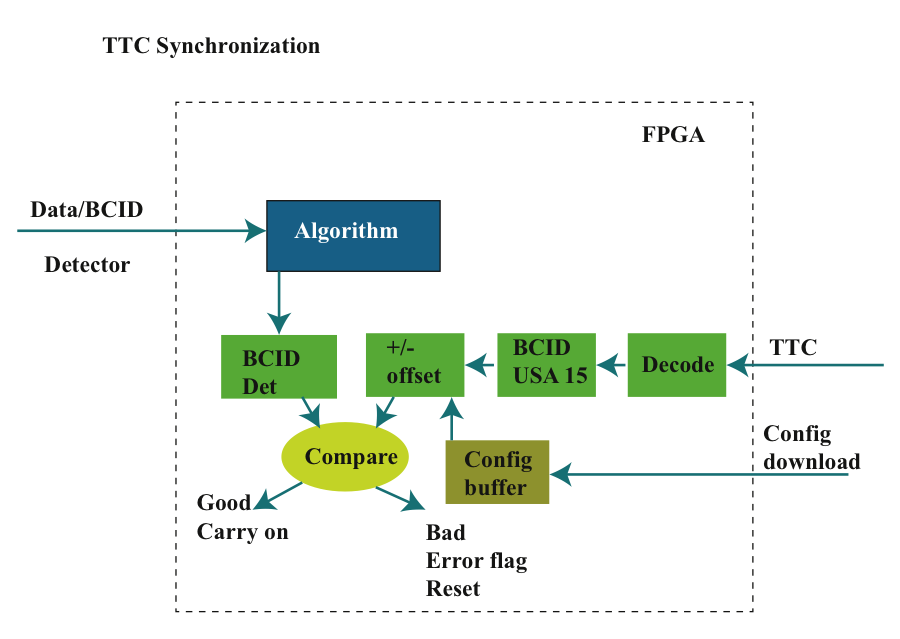
\includegraphics[width=0.8\textwidth]{specs/Diagram-TTCSync}
 % \caption{Block diagram of an implementation of the TTC synchronization.}
 % \label{fig:Monitoring}
 % \end{center}
 % \end{figure}


The ART (address in real time) data from an entire sector will be transmitted to a single
trigger processor via 32 ADDCs. Each ADDC will transmit its data on a
single fiber optic link. The trigger processor therefore uses 32
fibers to receive the ART data from one sector. The
MM and sTGC trigger processors will share the same ATCA carrier card
and each carrier will support two sectors.

\subsubsection{ART Data Protocol}

The ART Data from the ADDC will be transmitted using the GigaBit Transceiver
(GBT) architecture and transmission protocol in a low-latency widebus
mode at a rate of 4.8 Gb/s. The trigger processor will take advantage of the GBT firmware
developed by the GBT Project to implement the receivers.

The GBT packet in widebus mode will provide 112 data bits and arrives
once every bunch crossing. One ADDC will service 32 VMMs and each
packet can contain ART data from a maximum of eight triggered VMMs. Each
VMM will be uniquely identified to determine which MM strip
on the sector is hit.

There are two options for how data packet bits is defined. The
difference between the two is how the VMM ID information is encoded.
The first data protocol option will provide the VMM IDs of every VMM
that was triggered by asserting a bit in a 32-bit hit list as shown in 
Figure~\ref{fig:addcGbtFormat2}. The second
option will encode each VMM ID in a list. For both options, the triggered
strip number within each VMM will be provided in an encoded list. The first
option would move the VMM ID encoding task from the ADDC ASIC to the
trigger processor FPGA. 
Both options, shown in Tables~\ref{tab:ARTfmt_opt1} and
~\ref{tab:ARTfmt_opt2}, use the full 112~bits provided by the GBTx' wide mode.

\begin{figure}[h]
  \begin{center}
    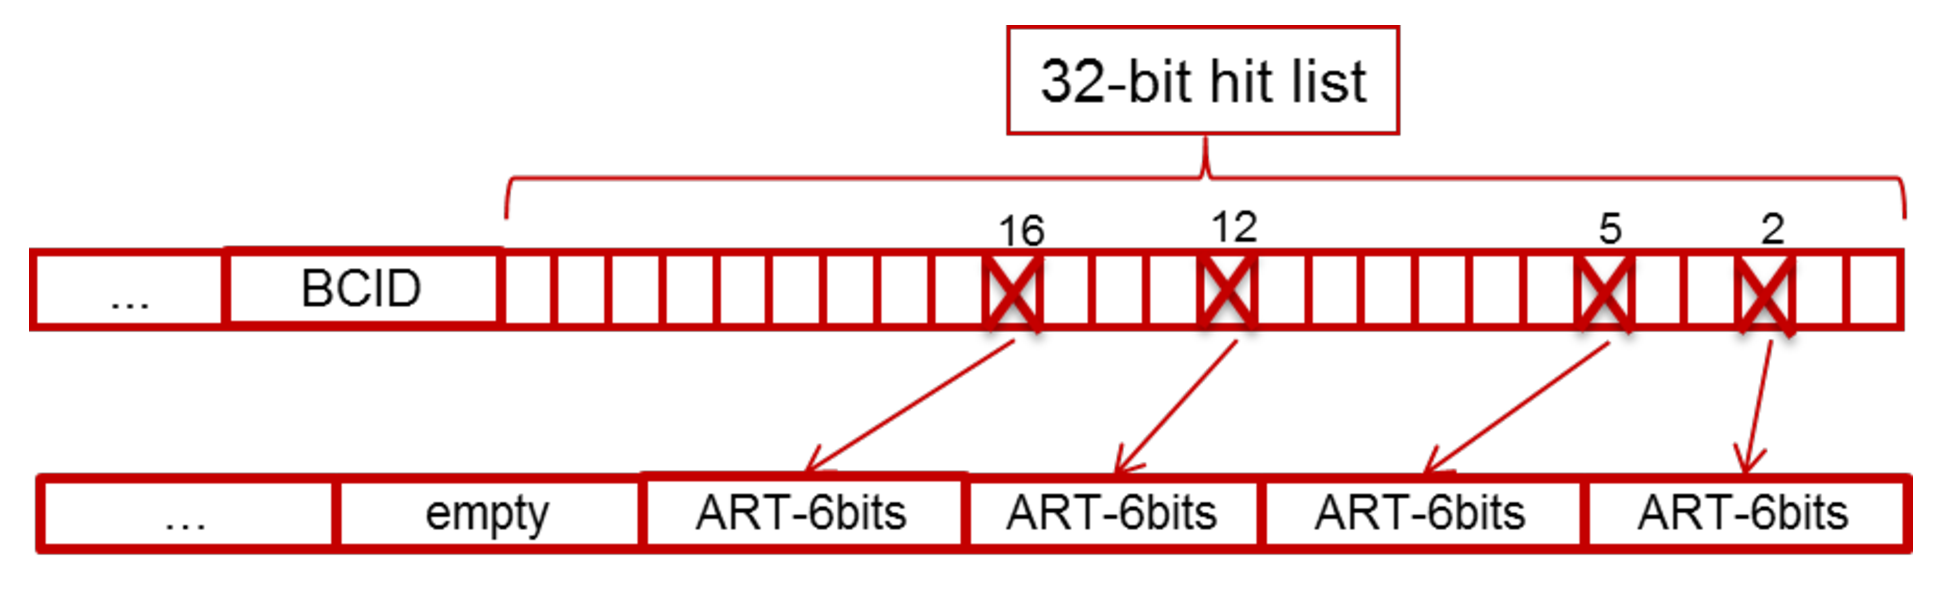
\includegraphics[width=0.6\textwidth]{figures/specs/addcGbtFormat2.pdf}
    \caption{Option 1 VMM ID encoding using 32-bit hit list.}
    \label{fig:addcGbtFormat2}
  \end{center}
\end{figure}


\begin{table}[htbp]
  \centering
    \begin{tabular}{|c|c|c|c|c|c|}
    \hline
    0b1010 & BCID(12) & ERR\_FLAGS(8) & HIT\_LIST(32) & ARTDATA\_PARITY(8) & 8xART\_DATA(6) \\
    \hline
    \end{tabular}\caption{Option 1 ADDC GBT packet format.}
  \label{tab:ARTfmt_opt1}%
\end{table}%

\begin{table}[htbp]
  \centering
    \begin{tabular}{|c|c|c|c|c|}
    \hline
    HIT\_CNT(3) & BCID(12) & 8xVMMID(5) & ARTDATA\_PARITY(8) & 8xART\_DATA(6) \\
    \hline
    \end{tabular}\caption{Option 2 ADDC GBT packet format.}
  \label{tab:ARTfmt_opt2}%
\end{table}%


\begin{comment}
{\small
\begin{tabular}{|c|c|c|c||c|c|}
\hline
\multicolumn{6}{|c|}{Option 1 GBT DATA{[}111:0{]}}\tabularnewline
\hline
\hline
``1010''  & BCID{[}11:0{]}  & ERR\_FLAGS{[}7:0{]}  & HIT\_LIST{[}31:0{]}  & ART\_PARITY{[}7:0{]}  & 8 x ARTDATA{[}5:0{]}\tabularnewline
\hline
\end{tabular}

\begin{tabular}{|c|c|c||c|c||c|}
\hline
\multicolumn{6}{|c|}{Option 2 GBT DATA{[}111:0{]}}\tabularnewline
\hline
\hline
HIT\_CNT{[}3:0{]}  & BCID{[}11:0{]}  & \multicolumn{2}{c|}{8 x VMMID{[}4:0{]}} & ART\_PARITY{[}7:0{]}  & 8 x ARTDATA{[}5:0{]}\tabularnewline
\hline
\end{tabular}
}  % end small

\end{comment}

%\begin{description}
%\item [BCID] = 12 bit bunch crossing ID 
%\item [HIT\_LIST] = 32-bit list of flags corresponding to each of
%the 32 VMMs. 0 - no hit, 1 - hit. A register controls if this is a
%filtered (i.e. 8 hits max) or an unfiltered copy of the VMM flags
%registered in a particular BC.
%\item [HIT\_CNT] = 4-bit  number of hits (range 0 - 8; 9 - 15 invalid)
%\item [VMMID] = 5-bit address of triggered VMM
%\item [ART\_DATA] = 6-bit triggered VMM strip number
%\item [ARTDATA\_PARITY] = 8-bit parity the ART data computed by
%each of the 32 ART de-serializer units. Each bit corresponds to one
%of the ART data field selected by the priority unit.
%\end{description}

\begin{itemize}
\item BCID = 12 bit bunch crossing ID 
\item HIT\_LIST = 32-bit list of flags corresponding to each of
the 32 VMMs. 0 - no hit, 1 - hit. A register controls if this is a
filtered (i.e. 8 hits max) or an unfiltered copy of the VMM flags
registered in a particular BC.
\item HIT\_CNT = 4-bit  number of hits (range 0 - 8; 9 - 15 invalid)
\item VMMID = 5-bit address of triggered VMM
\item ART\_DATA = 6-bit triggered VMM strip number
\item ARTDATA\_PARITY = 8-bit parity the ART data computed by
each of the 32 ART de-serializer units. Each bit corresponds to one
of the ART data field selected by the priority unit.
\end{itemize}


\subsubsection{Decoding ART Data}

Once the ADDC GBT packet is received, the ART data is decoded into a strip number.  This number represents the  strip's distance to the beam line.  Each fiber will have an associated  geographic address that is used in the decoding process to set the location of strip 0.  The strip number is then multiplied by a constant to calculate the slope of a line with the interaction point.  The slopes for each ART hit are then sent, along with the strip number, to the trigger processor algorithm.
Since the fiber location will provide information used to calculate the strip number, the ADDC will have a debug mode that can be used to diagnose cabling issues.

%-------------------------------------------------------------------------------
\subsection{Interface to sTGC}
\label{sec:specs-stgc}
\input{inputs/specs-stgc}

%-------------------------------------------------------------------------------
\subsection{Interface to Sector Logic}
\label{sec:specs-sl}
%
% Interface to Sector Logic
%

The track vector information from the NSW is combined with the results from the Big Wheel TGC (BW-TGC) by the new Sector Logic board located in USA-15.
The partitioning of the Trigger Sectors and granularities of the Regions-of-Interest (RoI) for the new Sector Logic board are the same as for the current \PhaseZero\ system. The same optical links and data format is used for signals from the BW-TGC, while new input optical links have been introduced to receive the NSW trigger information.

The BW-TGC, which covers the range of $1.0 < |\eta| < 2.4$, consists of three stations (TGC1, TGC2 and TGC3). The trigger algorithm extrapolates pivot-plane (TGC3) hits to the IP to construct roads following the infinite-momentum (straight) path for a track.
Deviations ($\Delta R$ and $\Delta\phi$) from this path of hits in the trigger planes are related to the momentum of the track.
Coincidence signals\footnote{The TGC1 station has three layers and the outer two stations (TGC2 and TGC3) each have two layers, resulting in a total of seven layers. A 3-out-of-4 coincidence is required for the doublet planes of TGC2 and TGC3, for both wires and strips; a 2-out-of-3 coincidence is required for the triplet (TGC1) wire planes; and 1-out-of-2 possible hits for the triplet strip planes.} are generated independently for $R$ and $\phi$.
The hit position information with granularity of RoIs and deviations ($R$ and $\Delta\phi$) is sent to the Sector Logic board.

The NSW information on the candidate track vectors, which are pointing to the IP within $\pm (7 - 15)$~mrad deviations\footnote{The value of this requirement is configurable and it will be optimized once better trigger simulation is available.}, are provided to the Sector Logic: the position ($R$ and $\Delta\phi$) and the deviation of the incidence angle at the NSW from a straight line to the IP ($\Delta\theta$).
In \PhaseOne, the final trigger decision is taken solely by merging the $R - \phi$ coincidence of signals from the BW-TGC and the NSW. In \PhaseTwo, the $\Delta\theta$ information will be combined with similar information from the BW chambers to improve the background rejection and sharpen the trigger threshold.
Since the NSW trigger system needs to be compatible with the \PhaseTwo requirements, the angle $\Delta\theta$ is required to be measured with an accuracy close to 1\,mrad even in \PhaseOne.


\subsubsection{NSW Trigger Data Format}
\label{ssec:specs-TriggerFormat}

The output data format of a track segment from the NSW trigger processor is shown in Table~\ref{tab:DataFormat}. One track segment is represented as 24~bits of data, which consist of 2~bits of segment-type information for each detector (\stgc and \MM), 5~bits for $\Delta\theta$, and 6~bits and 8~bits for $\phi$ and $R$ position information, respectively. Required resolutions (1~bit) are approximately 1~mrad ($\pm$15~mrad full scale) for $\Delta\theta$, 20~mrad for $\phi$ and 0.005 in pseudo-rapidity $\eta$.

The 2-bit segment-type information can provide an indication of the segment candidate quality, in addition to the detector. A value other than 00 indicates the segment was found by the corresponding detector. Up to a 3-level categorization can be encoded (01, 10 and 11), but the specific definitions are not yet established. 

Even though the sector logic is blind to the track segment origin (either \MM or \stgc) and quality, the segment-type bits should still be transmitted. They can be used to monitor the trigger operation, $e.g.$ to study the BW matches for each segment-type. The latency saved by omitting these four bits per candidate is small.


\begin{table}[h]
    \begin{center}
    \begin{tabular}{|c|c|c|c|c|c|c|}
    \hline
    Field:     & sTGC type & MM type & $\Delta\theta$ (mrad) & $\phi$ index &  $R$ index  &  spare  \\
    \hline
    Num of bits: &    2    &    2     &     5    &    6    &    8   &  1 \\
    \hline
    \end{tabular}
    \end{center}
    \caption{Data format of the output of the trigger processor sent to the Sector Logic. Format of a track vector candidate from the NSW (24-bits/track vector). The \stgc and \MM type information can encode the quality of the candidate.}
    \label{tab:DataFormat}
\end{table}


The data is transmitted from the \stgc and \MM trigger processors to the Sector Logic via optical fibres. The baseline is to send eight candidates per LHC bunch crossing (40~MHz) on two fibers, four candidates per stream, at 6.4\,Gb/s, 128~bit, using 8b/10b encoding. Figure\,\ref{fig:DataFormat} shows the format of the transmitted data. It is comprised of two IDLE codes for alignment purposes, three bytes of data for up to four track segments, the NSW Sector ID (4~bits) and a BCID number (12\,bits). Each 2-byte word is transferred after 8b/10b encoding at 320\,MHz.


\begin{figure}[h]
    \begin{center}
        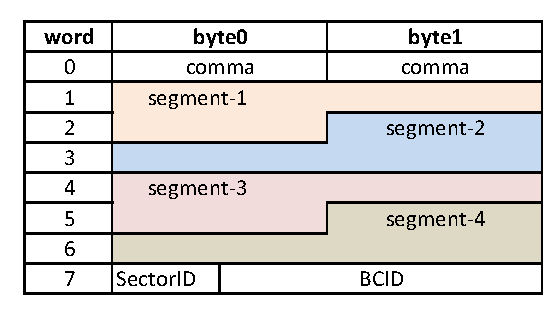
\includegraphics[width=0.55\textwidth]{specs/NSWtoSectorLogicFmt.pdf}
        \caption{Data format from the NSW trigger processor to the Sector Logic. The data is transmitted with 8b/10b encoding in one bunch crossing (16\,bytes at 6.4\,Gbps). The 24-bit segment format is shown in Table~\ref{tab:DataFormat}. The comma character is an idle code for alignment purposes in the 8b/10b encoding.
        The NSW Sector ID is 4~bits and the BCID is 12~bits.}
        \label{fig:DataFormat}
    \end{center}
\end{figure}

%The model of the trigger in the Athena simulation of both the sTGC and the MM trigger is incomplete. There is also a need to simulate correlated backgrounds. As a result, the probability to find track segments as a function of the radius is not known. The main quantities of interest are the probability of finding more than four \stgc or \MM candidates, as well as more than eight total candidates when duplicates are removed.

\paragraph{Data overflow}Information about data overflow is planned to be added. An overflow bit would be set if, for a BCID, more than the maximum number of transmittable candidates is found, and thus incomplete information is sent. One possibility is to use the reserved bit of the last track candidate word sent to the Sector Logic. This option requires no additional bits. 

If the simulation shows that eight candidates are insufficient, the following possibilities, although highly undesirable, could be considered to enable transmitting up to 12 candidates:
\begin{itemize}
\item Increase from two to three fibres. This option would exceed the number of serializers available with the intended Kintex FPGA and increase the complexity of the Sector Logic.
Recently, however, it was found that the Sector Logic boards may in fact be able to handle up to 10 links from the NSW, instead of six, as initially thought. This means that a third fiber might be available in case of need. More studies would be necessary to explore the eventual use of this possibility, which is not our baseline.
\item Transmission at 9.6 Gb/s, however the Kintex GTX cannot operate at this rate (higher or lower is OK). Note that this does not require any change at the Trigger Processor end.
\item Transmission at 8 Gb/s which would be sufficient to provide 10 candidates.
\end{itemize}


\subsubsection{Combination of sTGC and MM trigger data}
\label{ssec:specs-combination}
% Combination of sTGC and MM trigger data
%

The \MM and \stgc trigger processors compute track vectors independently. The \stgc trigger produces a maximum of four candidates per sector, driven by its hardware design.
The \MM trigger has no such limitation and can theoretically find more candidates if they are present. 

%Both \stgc and \MM trigger processors belonging to a NSW \sector will be in the same ATCA board~\cite{hardware-LAr-Carrier,hardware-SRS-Carrier}, although their information is processed by separate algorithms (see Section~\ref{sec:algorithms}) in separate FPGAs. 

The \stgc and \MM trigger information from one NSW \sector will be processed in the same Trigger Processor ATCA board~\cite{hardware-SRS-Carrier,hardware-LAr-Carrier}. The two algorithms (see Section~\ref{sec:algorithms}) will run in separate FPGAs, connected by several high-speed, low latency differential LVDS pairs.
Depending on the hardware platform chosen the two FPGAs will be located in one (SRS option~\cite{hardware-SRS-Mezz}) or two  (LAr option~\cite{hardware-LAr-OTC}) mezzanine cards. 
A NSW trigger processor ATCA board serves one NSW octant, i.e. two NSW sectors, and therefore
contains two or four mezzanine cards (depending on the hardware platform).
A comparison of the two platforms is provided in Section~\ref{sec:hardware-platforms}.

%A NSW trigger processor ATCA board (corresponding to two NSW sectors) contains two or four mezzanine cards (depending on the hardware platform ultimately chosen) and therefore serves a NSW octant

Given that the \MM trigger system is expected to be faster than the \stgc one, the \MM trigger results will be sent 
to the \stgc FPGA for the stream merging stage. This procedure eliminates the impact on the latency due to the data transfer. The merging algorithm, which includes duplicate removal, is expected to take up to 50 ns, 
increasing the overall NSW latency budget to 43 BCs. The actual algorithm implementation is however needed for a full evaluation of its impact on the latency.

In order to implement the merging algorithm, the fast connectivity between the \MM and \stgc FPGAs is imperative.
In the current design, the SRS option offers 64 LVDS high-speed connections between the FPGAs, which would fully satisfy the bandwidth requirements, while the LAr option only offers eight.
Studies are on-going to determine by how much this number could be increased.

The trigger stream merging will limit the number of NSW track vector candidates to eight (subject to simulation results, see Section~\ref{ssec:specs-TriggerFormat}). Possible selection criteria of track vectors are:
\begin{itemize}
	\item Remove duplicates, where a duplicate is a candidate with the same $R$ and $\phi$, and similar $\Delta\theta$. The conditions for a $\Delta\theta$ match still need to be evaluated taking into account the intrinsic resolutions and the relative alignment of the two detectors.
	\item Select according to a `quality' flag defined by the trigger algorithm. For example, if the vector was produced from only one of the two four-layer modules of the \stgc because the track passed through a support in the second module, its resolution is degraded and the vector would have a lower quality.
\end{itemize}

Although both \stgc and \MM trigger modules are in the same ATCA board with high bandwidth connectivity, an algorithm that would merge hits and then find vectors has been disfavored at this time due to the additional latency requirements and increased complexity.

%Handling the details of the detector differences at the hit level would require more processing time than is available in the \PhaseOne latency budget.
%Any improvement of the vectors' accuracy from such an algorithm may not be needed, at least for \PhaseOne, and the added complexity may not be justified.


\subsubsection{Matching to Sector Logic Boards}
\label{ssec:specs-sl-boards}

Figure~\ref{fig:L1MuEC-TriggerSector} shows the projection of the NSW sectors into the BW-TGC pivot plane which is divided into two regions, end-cap ($|\eta|<1.9$) and forward ($|\eta|>1.9$). The end-cap region is divided into 48 trigger sectors in $\phi$, while the forward region is divided into 24 trigger sectors. A trigger sector, represented in the figure by the green lines, is a logical unit that is treated independently in the trigger\footnote{Remember that the TGC has 12 detector sectors. Thus, each TGC detector sector comprises four end-cap trigger sectors and two forward trigger sectors.}.

The thick red lines in Figure~\ref{fig:L1MuEC-TriggerSector} show the projective boundaries of the NSW detector, which covers $1.3<|\eta|<2.4$ and whose structure has octant symmetry. 
Each octant has a large NSW sector and a small NSW sector\footnote{Note that in the NSW the detector and trigger sectors are coincidental, unlike in the case of the BW-TGC.}, corresponding to 16 NSW Trigger Sectors per endcap. 
The boundaries of the NSW sectors (indicated by the red lines) do not coincide with the segmentation of the BW-TGC trigger sectors. Each large NSW sector geometrically covers six BW-TGC Trigger Sectors, while each small NSW sectors covers seven (notice the very thin overlap regions in the NSW small sector case). 

To take into account deformations in the endcap magnetic field, multiple scattering and misalignments, one NSW sector also needs to deliver information to the BW-TGC sectors adjacent to the geometrically overlapping ones.
This means that the information from a large NSW sector has to be corroborated with that of six \endcap trigger sectors and four forward trigger sectors.
Similarly, information from a small NSW sector has to be combined with four \endcap trigger sectors and three forward trigger sectors.

The granularity of the Regions-of-Interest is indicated by the thin red lines. The sizes of the RoIs are approximately 0.025$\times$0.030 in \etaphi. There are 560 (366) RoIs corresponding to each large (small) NSW sector.
%{\bf (I counted a slightly different number: large - (12+14)*4*4 + 16*4*2 = 416 + 128 = 544; (12+14)*5*2 + 16*6 = 260 + 96 = 356).}

\begin{figure}[htb]
  \centering
  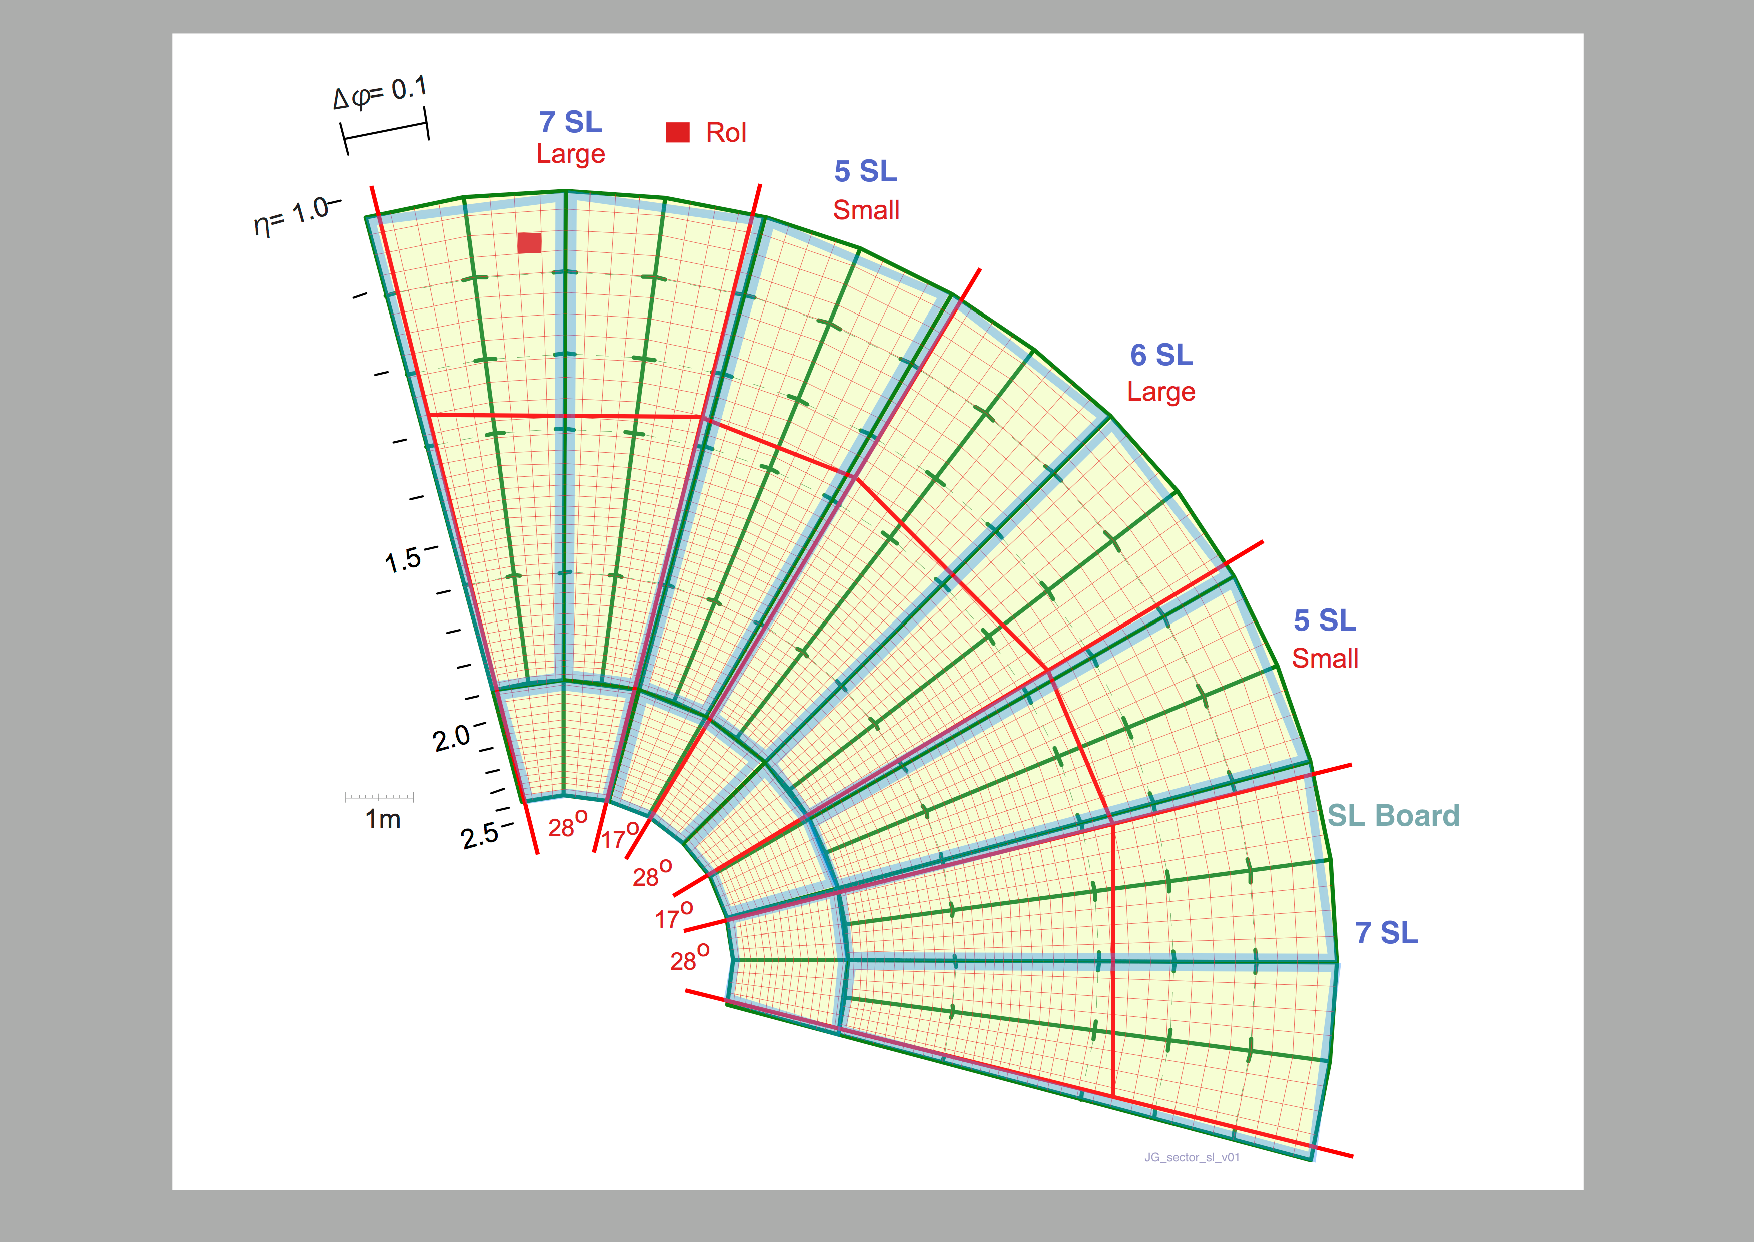
\includegraphics[trim=4cm 1.0cm 4.7cm 1.0cm, clip=true, width=0.8\textwidth]{specs/JG_sector_sl_v01.pdf}
  %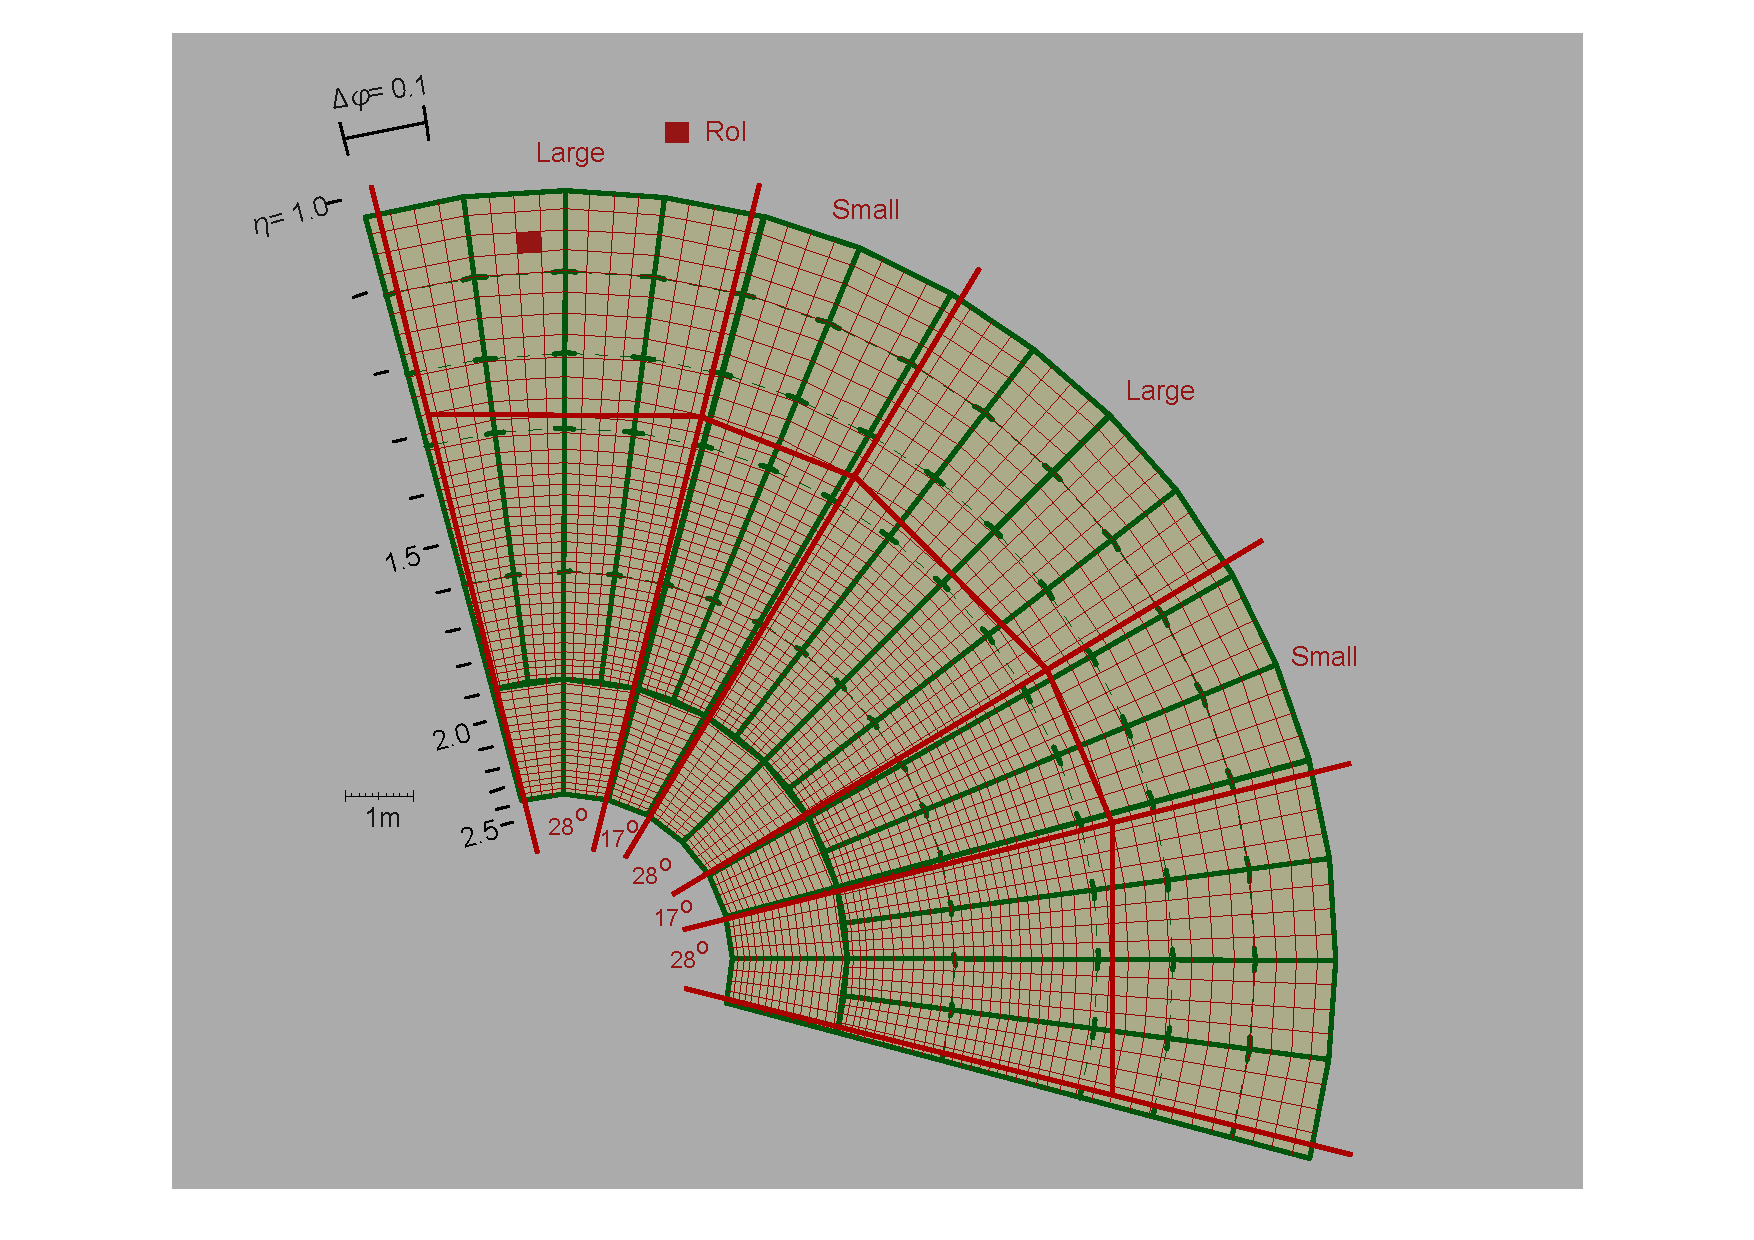
\includegraphics[trim=4cm 1.0cm 6.5cm 1.0cm, clip=true, width=0.7\textwidth]{specs/sector.pdf}  
 \caption{Trigger Sector segmentation (green lines) and projection of the NSW sectors (thick red lines) into the pivot plane (TGC3). The blue shapes represent the coverage of a SL board. The number of SL boards covered by each NSW sector is indicated in blue.}
  \label{fig:L1MuEC-TriggerSector}
\end{figure}

There are two types of Sector Logic boards, the ``\Endcap Sector Logic'' board and the ``Forward Sector Logic'' board. A single Sector Logic board serves two adjacent trigger sectors, therefore 24 Endcap and 12 Forward Sector Logic boards per side are required.
Figure~\ref{fig:L1MuEC-TriggerSector} shows the mapping of the SL boards (in blue) to the trigger sectors. The trigger information from each NSW trigger sector is fanned-out and delivered to the corresponding SL boards. There will be five to seven replicas required from each NSW sector because a single SL board serves two trigger sectors. 
This maximum number of signal fan-out is needed for the NSW large sector.



%Figure~\ref{fig:L1MuEC-FanoutScheme} shows the signal distribution scheme from the NSW to the Sector Logic
%boards. Vector data of track segments, which are found in sTGCs and MicroMegas separately, are merged by the NSW trigger electronics. Combined track information is fanned-out and delivered to corresponding Sector Logic boards.

Several replication possibilities are currently being considered:
\begin{description}
    \item [1:7 fan-out with active fan-outs:] slightly higher latency due to optical-electrical-optical conversion and additional fiber length
    \item [1:7 fan-out with passive optical splitter:] rejected since signal loss is too high
    \item [2$\times$(1:4) passive optical splitter:] perhaps possible, depending if the transmitter optical power is sufficient. Would need to be checked and/or tested.
    \item [4$\times$(1:2) passive optical splitter:] OK, but only if the trigger processor has enough outputs.  Requires eight output optical links.
    \item [7 fibers directly from TP:] OK, but only if the trigger processor has enough outputs. Requires 14 output optical links.
\end{description}

At this point, both platform options should be able to provide 14 optical output links for this purpose. Pending a deeper evaluation, the baseline is that the TP will provide the seven streams (2 x 7 fibers) directly to the SL, without the need for a fan-out, as shown in Figure~\ref{fig:Interface-TP-SL}.
Note however that neither the opto-electronics for additional links nor the fan-outs have been included in the NSW costing.

\begin{figure}[htb]
  \centering
  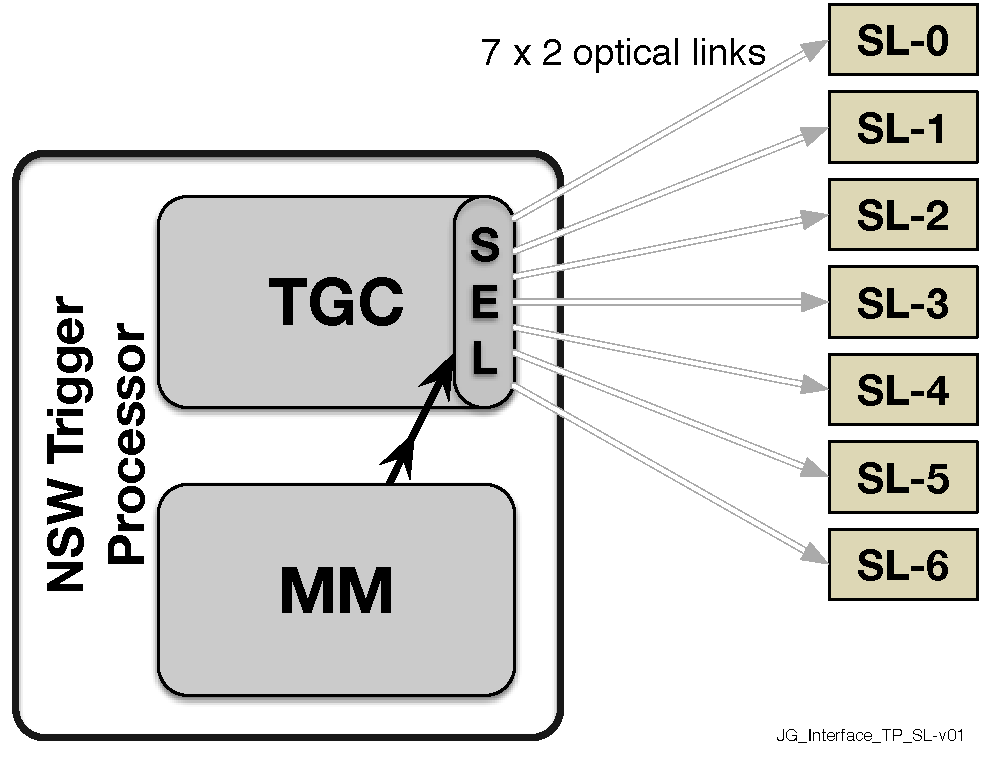
\includegraphics[width=0.4\textwidth]{specs/JG_Interface_TP_SL-v01}
 \caption{Interface between the NSW trigger electronics and the Sector Logic.
 One NSW trigger sector will connect to up to seven SL boards via optical links.}
  \label{fig:Interface-TP-SL}
\end{figure}


It has also been proposed that splitting the fibers, at the NSW Trigger Processor, as belonging to different $\phi$ regions within a sector might reduce the need to fan-out the output, without compromising the maximum number of candidates transmitted. This would however introduce undesirable hard boundaries into the SL. A third fiber from inner regions of the large sectors might also be used. More studies would be needed to explore these possibilities.


%{\bf Stuff below here is to be removed}
%
%\begin{enumerate}
%  \setlength{\itemsep}{1pt}
%  \setlength{\parskip}{0pt}
%  \setlength{\parsep}{0pt}
%        \item   Send trigger segments to Sector Logic
%        \begin{enumerate}
%        \item   Steps required
%        \begin{enumerate}
%        \item   Construct $\Delta\theta$, and ROI locations of each candidate in appropriate format (as given in Figure~\ref{fig:DataFormat})
%        \item   Synchronize to BC domain and output on required BCID
%        \item   Serialize for transmission to Sector Logic using Xilinx GTX core
%        \begin{enumerate}
%        \item   Encode with 8b/10b (VHDL from FELIX)
%        \end{enumerate}
%        \end{enumerate}
%        \item   Failure modes and recovery
%        \begin{enumerate}
%        \item   Too many segments for transmission – truncate list to maximum allowed; send exception message.
%        \end{enumerate}
%        \end{enumerate}
%\end{enumerate}

\FloatBarrier

%-------------------------------------------------------------------------------
\subsection{Ancillary Functions}
\label{sec:specs-ancillary}
In addition to implementing the trigger algorithms for the \MM and
\stgc systems, the NSW Trigger Processor has to perform several
ancillary functions. These include time synchronization,
configuration, monitoring and debugging mode, among others. Several functions are common to both \MM and \stgc and their firmware can be shared as well-defined packages. These functions are:

\begin{description}

  \item[Interface for algorithm configuration parameters] \hfill \\
  Parameters for the algorithms must be stored at runtime. Examples
  are the $\Delta\theta$ and other cuts, the BCID offset, alignment
  parameters, the parts of the detector to be considered as disabled,
  road size, etc. Configuration can be done via Ethernet and the
  carrier board or via an E-link from FELIX that is available on the link that brings the TTC information.
  Readback of the parameters must also be provided.

  \item[TTC interface] \hfill \\
  FELIX provides the following TTC information on an E-link: \\
  \hspace*{5mm} Level-1 Accept, BCR, ECR, system[3..0], user[7] from the 8-bit TTC broadcast packet \\
  The E-link provides the 40\,MHz BC clock which is used to
  synchronize the output to the Sector Logic. This also includes the logic to synchronize a local bunch-crossing ID to the Sector Logic
  by means of a configurable BC offset loaded on BCR into a local BCID register.
  Note that the various input links will not have the same phase and may not even be matched to the same BC clock.
  Input processors must ensure that all sources are aligned to the same BC clock.
  Both technologies include a BCID or its low bits in the packet sent on every bunch-crossing.
  Should the offset of this BCID from the local BCID differ from what is expected, an exception message (see below) must be sent.
  The firmware to do this alignment is not shared.

  \item[Level-1 output buffer] \hfill \\
  For bunch-crossings in which at least one segment is found,
  the input data and the output segment data that is sent to the Sector Logic is stored,
  along with its BCID for later matching to the BCID of a Level-1 Accept.
  Those bunch-crossings that have Level-1 Accepts (and possibly those preceding and following) are transferred to the Level-1 output buffer (aka derandomizer).
  The data must be stored for the duration of the Level-1 latency.
  The output bandwidth should be sufficient for the rather small fixed input and output data lengths at the full Level-1 rate of 400\,kHz.
  If not, this logic could provide a BUSY output to the RODBUSY system when its output buffer becomes close to full.

  \item[Monitored event buffer] \hfill \\
  A random sample of complete events are collected for sending to a monitoring process.
  Example criteria are: any event, event with at least one segment found, events with segments outside the $\Delta\theta$ cut, \ldots\.)
  The data buffered as one event includes all the input data and the output segment data that is sent to the Sector Logic for a given BC.

  \item[Statistics buffer] \hfill \\
  Statistics are continuously collected and periodically transferred to the Statistics buffer.
  Statistics includes the number of bunch-crossings that have candidates that are not accepted by Level-1, their distribution in $R\phi$,
  the multiplicity of segments per bunch-crossing, etc.

  \item[Exception buffer] \hfill \\
  In the course of processing, exceptional conditions may be found, usually due to corrupted data.
  A convenient way to handle these is to store an exception code and some context data into a buffer which will be passed to the monitoring PC via FELIX.

  \item[Playback mode to fake input links] \hfill \\
  For development and testing we require that simulated data can be injected in place of the data received by the links to the Front End.
  One way to do this is via an E-link from FELIX that is available on the link that brings the TTC information.
  Full-speed testing.

  \item[Segment output to Sector Logic and to the ``other'' detector] \hfill \\
  Segments are sent out either to the Sector Logic via the FPGA serializer or to the ``other'' detector via a parallel LVDS bus.
  The candidate packet to be sent to the Sector Logic must be prepared from the segments found.
  Clones must be made and the output links to the Sector logic must be driven.
  If the segments found are to be sent to the ``other'' detector's Trigger Processor,
  the segment data must be sequenced out onto the parallel LVDS bus.

  \item[Merge buffers into the output GBT link to FELIX] \hfill \\
  The Level-1, Monitoring, Statistics and Exception buffers are merged, using different FELIX ``stream-IDs'' onto a fiber link to FELIX.
  FELIX then routes them to the ROD and Monitoring PCs.
  % This may use the FELIX, so-called, ``flat'' mode (not one of the GBTx modes), where data is streamed in 8b/10b encoding on a single

\end{description}

Since the MM uses the GBTx to transmit the data from the Front End and the sTGC uses native FPGA serializers,
the link interface firmware cannot be shared.
Note that the monitoring of board temperatures and voltages is done by the ATCA Shelf Manager using IPMI.
The fiber plant is described in Appendix~\ref{app:specs-fibers}.


%-------------------------------------------------------------------------------
%\subsection{Fibers Layout}
%\label{sec:specs-fibers}
%% Optical Fiber plant

\begin{figure}[h]
   \centering
   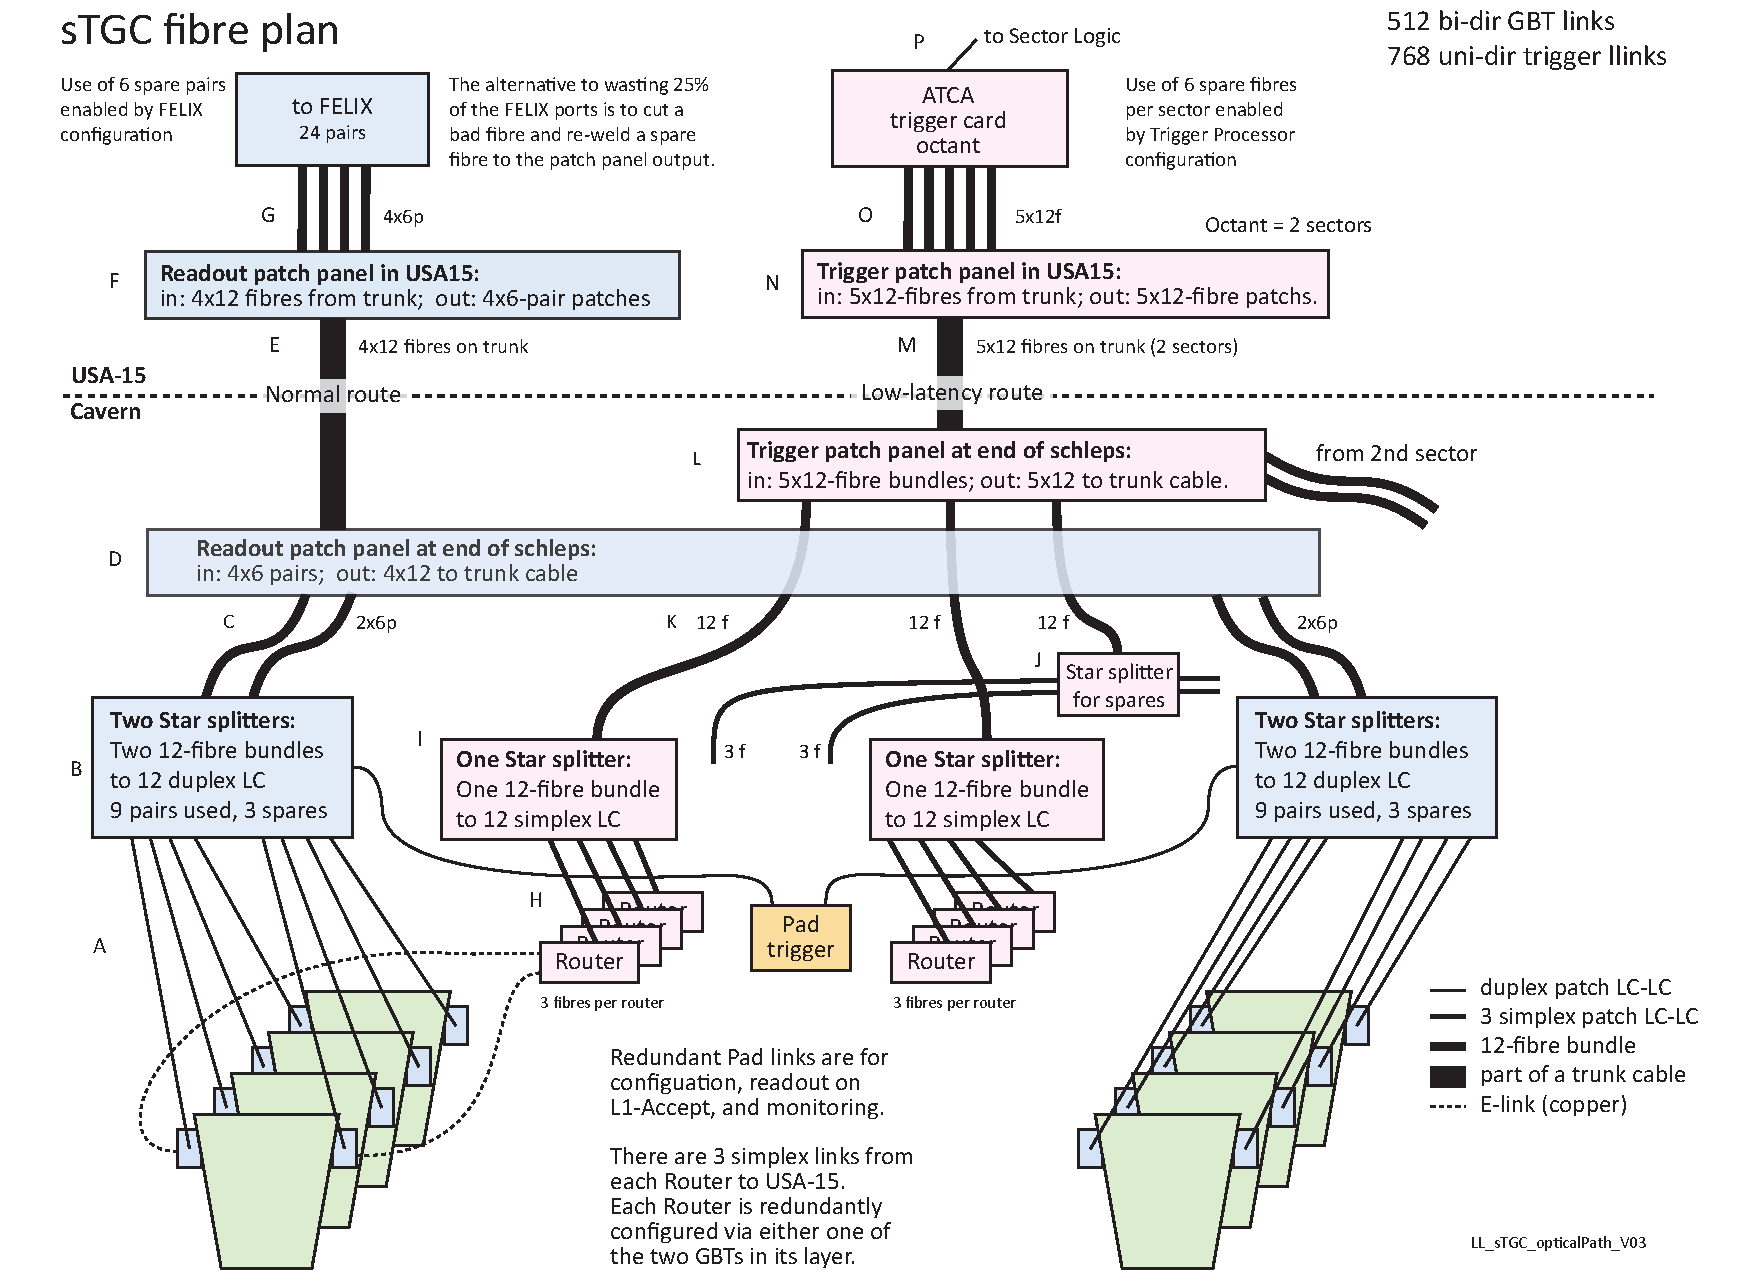
\includegraphics[width=0.99\textheight, angle=90]{figures/LL_sTGC_opticalPath_V03.pdf}
   \caption{Optical fiber plant for the sTGC, including both trigger and readout fibers.
   The current plan is for four fibers per layer (i.e.\ from each Router), instead of three.}
   \label{fig:LL_sTGC_opticalPath}
\end{figure}

\begin{figure}[h]
   \centering
   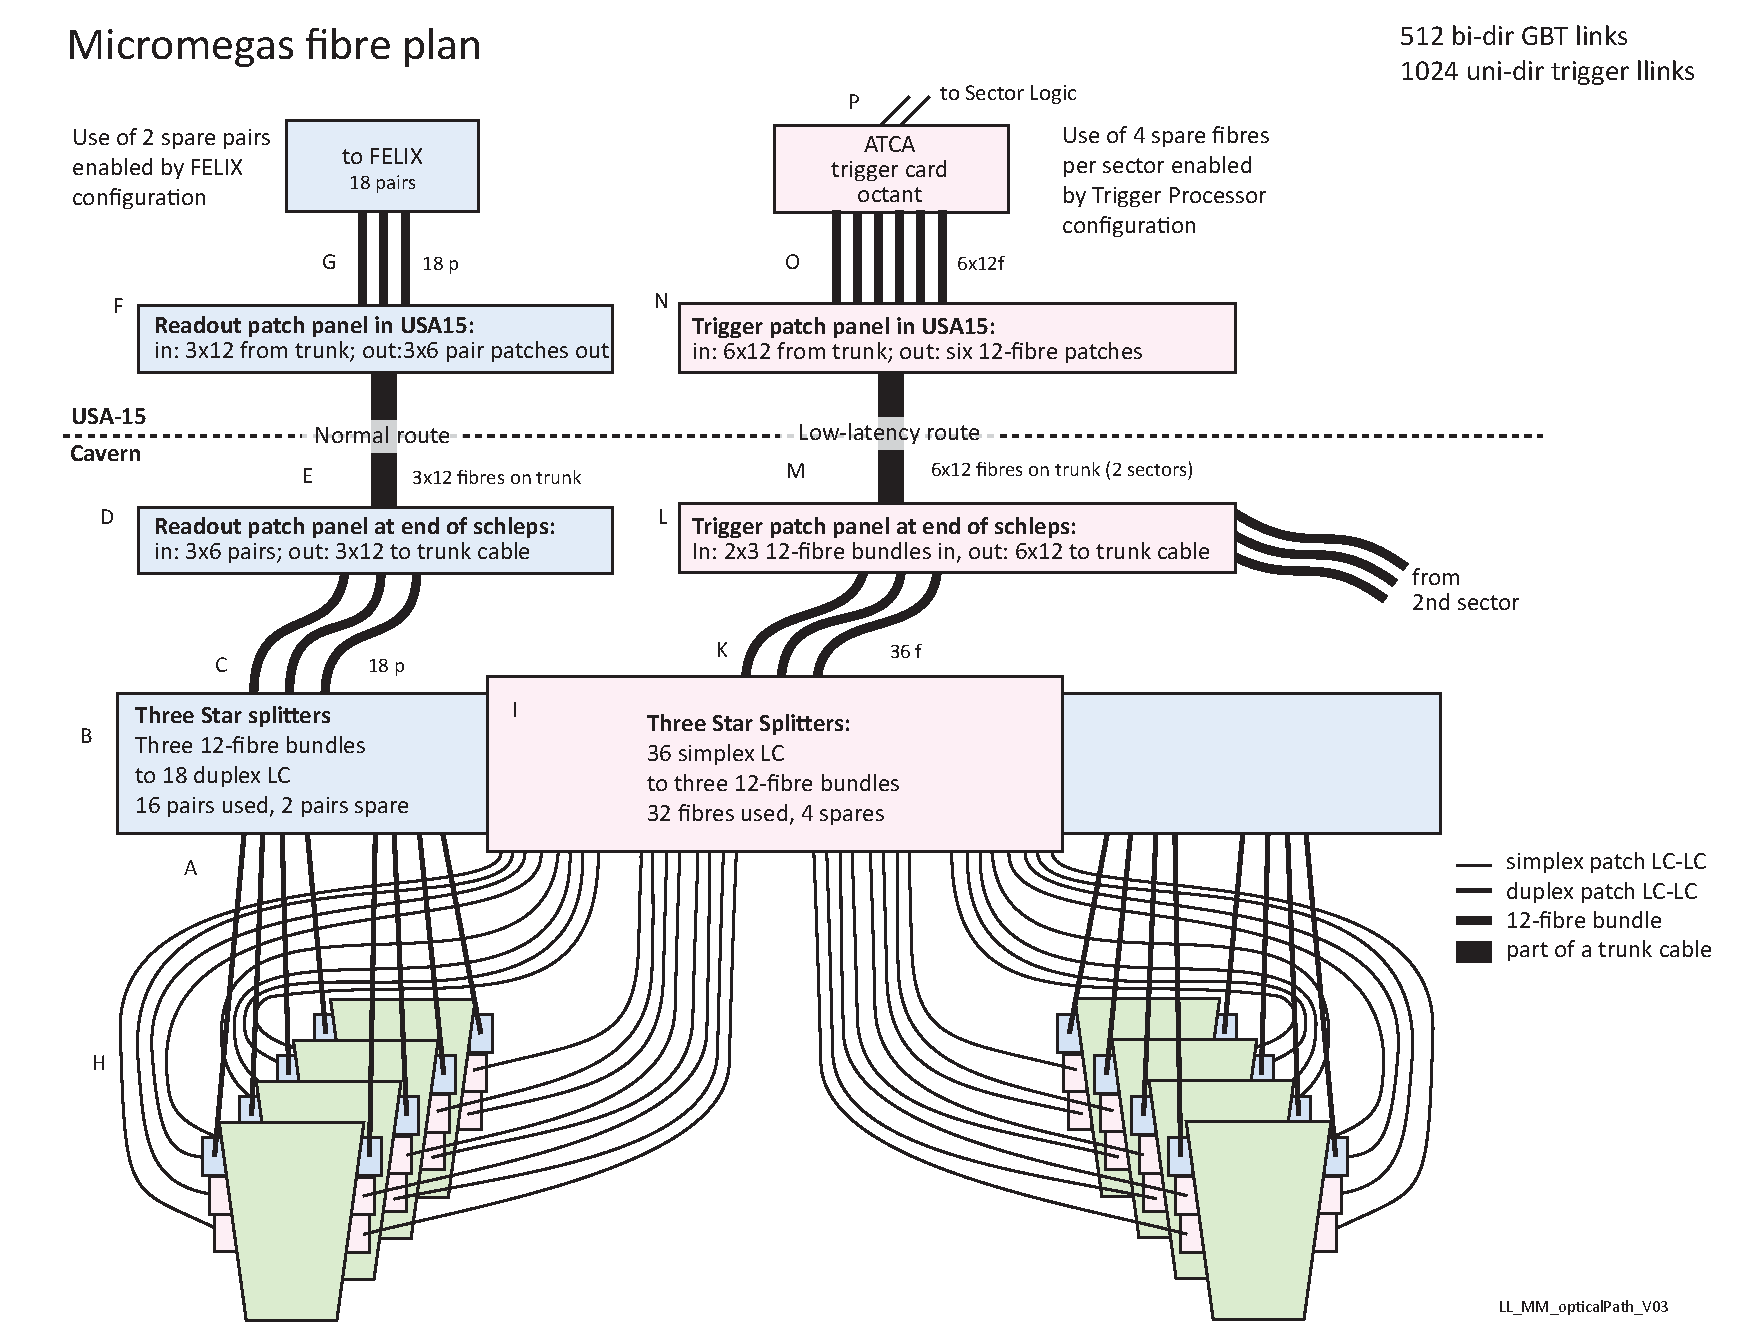
\includegraphics[width=0.99\textheight, angle=90]{figures/LL_MM_opticalPath_V03.pdf}
   \caption{Optical fiber plant for the Micromegas, including both trigger and readout fibers}
   \label{fig:LL_MM_opticalPath}
\end{figure}


\FloatBarrier

%-------------------------------------------------------------------------------

% Get all figures and tables to appear before moving into the algorithms
% The package placeins provides the macro \FloatBarrier to achieve this
\FloatBarrier

%-------------------------------------------------------------------------------
\section{Trigger Algorithms and Performance}
\label{sec:algorithms}
%-------------------------------------------------------------------------------
\subsection{Micromegas Trigger Algorithm}

Two \MM trigger algorithms are considered, the ``MM Fitter algorithm''
and the ``MM Look-Up-Table algorithm''. 
They are described in detail below in Section~\ref{sec:algorithms-harvard} and
Section~\ref{sec:algorithms-saclay} respectively.
Comparing and contrasting these algorithms will allow the development of an optimized final algorithm.

The \MM Fitter Algorithm is considered the baseline algorithm for now.
It is currently the one that has been investigated most extensively, including
studies on the impact of misalignments on its efficiency and resolution.
The algorithm is mostly complete and has been implemented on an FPGA evaluation board.
It is also the algorithm currently implemented in the ATLAS Trigger Simulation software.

The studies are however not complete since they do not include a proper background simulation, and in particular, effects from coherent background. 
A more realistic implementation of the trigger simulation is also required. 
Work is on-going on the trigger and cavern background simulations. Once these are finalized, we plan to test both algorithms with the conditions expected at high luminosity.
If the MM Look-Up-Table algorithm is shown to be more robust, changes to the final algorithm will be considered and implemented as necessary.


%-------------------------------------------------------------------------------
\subsubsection{MM Fitter Algorithm}
\label{sec:algorithms-harvard}
This section describes the algorithm introduced in Ref.~\cite{harvardAlg} and its performance.
It also includes details of its implementation on an evaluation board and measurements performed
using that setup, as well as recent studies of the impact of
misalignments on the algorithm performance.



%Note:   Trigger algorithm design and performance can be found in the note An Algorithm for Micromegas Segment Reconstruction in the Level-1Trigger of the New Small Wheels by Brian Clark et al., resident in CDS: https://cds.cern.ch/record/1706160

%%%%%%%%% Sample inclusion of a figure
 % \begin{figure}[h]
 % \begin{center}
 % \includegraphics[width=0.8\textwidth]{algorithms-harvard/Plot1}
 % \caption{Caption of plot 1}
 % \label{fig:Monitoring}
 % \end{center}
 % \end{figure}

\subsubsubsection{Description}
This algorithm has been described in detail in Ref.\,\cite{harvardAlg}. Here, its main features are
summarized. The algorithm has four functionally distinct sets of operations:
\begin{enumerate}\itemsep-5pt
\item translation of hardware addresses into equivalent track slopes fixed to the IP,
\item determination of the presence of a multi-plane coincidence,
\item parallel calculation of global $\theta$ (azimuth of the track position at the entrance of the NSW)
and local $\theta$ (direction, at the entrance of the NSW, referred to as $\theta_{rec}$ in Section~\ref{sec:algorithms-saclay}) 
angles with parallel strips and global average stereo strips, 
using the multi-plane coincidence,
\item calculation of $\Delta\theta$, global $\theta$ (referred to as $\theta$ in what follows) and $\phi$.
\end{enumerate}
The first two items are performed by many {\em finders}, which don't consume significant amount
of resources, but reduce significantly the throughput towards the second half of the algorithm. Items
3 and 4 are performed by {\em fitters} that consume most of the resources allocated to the algorithm,
but only performed upon the presence of a solid track candidate.
Figure\,\ref{fig:harvardAlg} shows the algorithmic flow with smaller functional units. They are labeled
for easy reference when discussing the algorithm implementation.
	\begin{figure}[htbp]
	\begin{center}
	\includegraphics[width=\textwidth]{algorithms-harvard/block_detailed_V02.pdf}
	\caption{\label{fig:harvardAlg} The block diagram is constructed with time flowing downward; therefore tasks on the same horizontal line are accomplished in parallel.  Blocks correspond to operations comprising the algorithm, solid flow lines represent the flow of data, and light dotted lines represent fit abandonment signals, which can be triggered at multiple points throughout the algorithm. X in this diagram refers to horizontal strips, while U and V refer to the two sets of stereo strips (with a $+1.5^{\circ}$ and $-1.5^{\circ}$ stereo tilt respectively). Blocks after step D are approximately sized to represent their relative processing times.}
	\end{center}
\end{figure}

\subsubsubsection{Implementation}\label{sec:harvard_impl}
A 1/16\textsuperscript{th} sector wide slice of the full algorithm above has been implemented and the design is being tested using a Xilinx VC707 Development board. This board includes a Virtex XC7VX485T FPGA. The implementation includes two ADDC GBT interfaces and associated trigger processor algorithm. Extrapolating from this implementation, the resources are estimated to be \textasciitilde{}70\% of the Xilinx V7\,485 chip.
There are pin-compatible upgrades to the target chip if more resources are needed.
Specifically, each of the steps shown in Figure\,\ref{fig:harvardAlg} has been implemented as follows.

\begin{enumerate}%[(A)]
\item[(A)] Incoming strip hit addresses are converted to global slope values using a multiplication with a constant. A strip's stored slope value is
defined as the orthogonal distance between a given strip and the beam line divided by the $z$ location of the relevant detection
plane. It is precomputed taking into account a strip offset and a $z$ position stored for each of the 8 planes and
16 radial segments of each wedge (one segment is read-out per MMFE8).
\item[(B)] Hit slope values are stored in a circular buffer defined as $(N$~slope-roads$)\times(8$~planes$)\times(T)$, where $T$ is the cyclical buffer depth and corresponds to the number of bunch crossings over which coincidences between planes are allowed.  A track candidate is identified once a minimum hit threshold is met. The value of $N$ has been optimized to maximize efficiency while being resilient to backgrounds\cite{harvardAlg}, and corresponds to about 4~(56) strips per slope road for horizontal (stereo) strips. 
Hits are kept in the buffer for a fixed number of bunch crossings that is configurable. For the studies in this document, two bunch
crossings are used. 
\item[(C)] Each slope-road of the buffer is checked once per bunch crossing to determine if a coincidence threshold has been met.
Coincidence requires a minimum number of planes to be hit and the oldest piece of data to be timing out. Coincidence identification is accomplished using the binary hit configuration for a given slope-road as the address of a lookup table that is pre-populated with pass or no-pass signals for various hit configurations of the eight planes.  Rather than searching the entire buffer for hits, only active areas are interrogated for confidence verification.
\item[(D)] slope-road contents containing the track candidate are read and cleared from the buffer and relevant track components are forwarded for processing. \\

\vspace{-4mm}
\hspace{-7.5mm} Once a candidate track is identified, the following steps (E-I) are completed in parallel: \\
\vspace{-4mm}

\item[(E)] A local slope is calculated using a least squares fit of available horizontal-strip hits in the proposed track.
Several constants are stored in a look-up table for the 11 possible combinations (indexed by $k=\{1..11\}$) of $n=\{2,3,4\}$
horizontal hits to speed up the fit ($M_X^{\rm local}$).
\item[(F)] A global horizontal hit slope, which is anchored to the IP, is calculated as the average of registered $n=\{2,3,4\}$ horizontal-strip hits in the proposed track candidate ($M_X^{\rm global}$).
\item[(G)] A global stereo (U) hit slope, which is anchored to the IP, is calculated as the average of registered $n=\{1,2\}$ U hits in the proposed track candidate.
\item[(H)] A global stereo (V) hit slope, which is anchored to the IP, is calculated as the average of registered $n=\{1,2\}$ V hits in the proposed track candidate.
\item[(I)] Stereo-strip background hits are further filtered from proposed tracks by judging how correlated two stereo-strip hits are with one another. In particular, strips with the same stereo tilt are compared between the two multiplets. If they are consistent between
the two multiplets, the pair is kept, while otherwise it is discarded. If only one multiplet registers a hit on a strip of a given stereo tilt, it is kept.
\item[(J)] $\Delta\theta$ is calculated using previously fitted local and global horizontal slopes ($M_X^{\rm local}$ and $M_X^{\rm global}$).
This calculation is accomplished using a small $\phi$ angle approximation. In local coordinates, for which $\phi=0$ at the middle
of the module, this approximation introduces at most a 4\% bias in the $\Delta\theta$ calculation.
In order to speed up the calculation, the quantity $1/(1+M_X^{\rm local}M_X^{\rm global})$ is calculated using a reciprocal
look-up table
that introduces a negligible error. Tracks with negative local slopes (originating from outside the detector) are rejected at this step.
Candidates with $\Delta\theta>15$~mrad are also rejected at this step.
\item[(K)] A $\theta$ and a $\phi$ are calculated using previously calculated stereo and horizontal slopes. In particular, if hits
exist for both stereo tilts, the cartesian position along the horizontal strip direction is calculated using the two
stereo hit slopes (U and V). If only one exists, the intersection point of the stereo strip and the horizontal strip is
calculated. This requires the storage of two quantities: $A\equiv\csc(1.5^{\circ})$ and $B\equiv\cot(1.5^{\circ})$, two products
and an addition. The horizontal slope provides the other cartesian coordinate. The two cartesian coordinates are transformed
into $\theta$ and $\phi$ using a look-up table. If the two cartesian coordinates do not correspond to a $\theta$ and $\phi$
in the wedge (which can happen in cases with significant background contamination), the candidate is rejected.
\item[(L)] A $\Delta\theta$, $\theta$ and $\phi$ are offered as a trigger signal.

\end{enumerate}

\paragraph{Latency}  
Timing estimates for these steps have been performed using the evaluation board described at the beginning of this
section. These estimates do not include the last look-up table to go from cartesian to cylindrical coordinates in step\,K.
The trigger algorithm's longest path is 56.25\,ns, assuming all necessary hits arrive promptly and track fitting
begins immediately. The splitting of the latency at each step of the algorithm in clock ticks is summarized in 
Figure~\ref{fig:harvard_latency}. 
	\begin{figure}[htbp]
	\begin{center}
	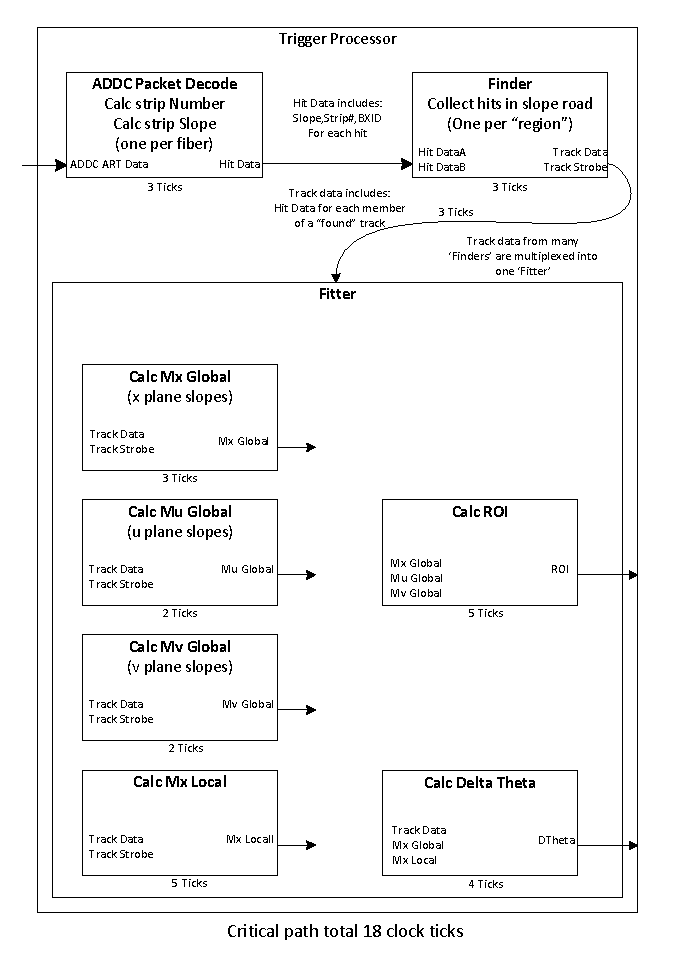
\includegraphics[width=0.7\textwidth]{algorithms-harvard/hdlBDv2.pdf}
	\caption{\label{fig:harvard_latency} Latency of the Harvard algorithm in clock ticks in each major step of the algorithm. }
	\end{center}
\end{figure} 
The last look-up table should only increase this latency by 1\,clock tick, that is to 59\,ns. Therefore, the latency time of the 
algorithm is slightly above two bunch crossings. 

\subsubsubsection{Misalignment Configurations and Corrections}

The performance in Section\,\ref{sec:harv-perf} is evaluated for ideal conditions and for
samples simulated with several misalignment effects. This section describes
the types of misalignment effects considered, how they are simulated and the
implementation of misalignment corrections in the FPGA algorithm. All misalignments
considered refer to misalignments of one multiplet with respect to the other in
the same sector. Misalignments affecting the full sector are not addressed, because they
only affect the $\theta$ and $\phi$ determination, which requires less precision. However, similar correction
techniques as those explored here can be applied to full sector position inaccuracies.

The following misalignment configurations are considered:
\begin{enumerate}\itemsep-4pt
\item $r$, displacements orthogonal to the beam axis---one or part of a multiplet shifted up or down with respect to the other,
\item $\phi$, rotations along an axis perpendicular to the wedge of one multiplet with respect to the other, with the axis
going through the center of the lower edge of the chamber,
\item $\theta_{\rm tilt}$, one plane tilted towards the IP with respect to the other,
\item $z$, one multiplet displaced along the beam axis.
\end{enumerate}
Figure\,\ref{fig:harvard_misal_illustration} illustrates each of these cases. Figures\,\ref{fig:harvard_misal_illustration}\,(a)
and~(b) correspond to two cases of the first misalignment type considered above.
\begin{figure}[htbp]
	\begin{center}
	\subfloat[a][Shift in $r$]{
		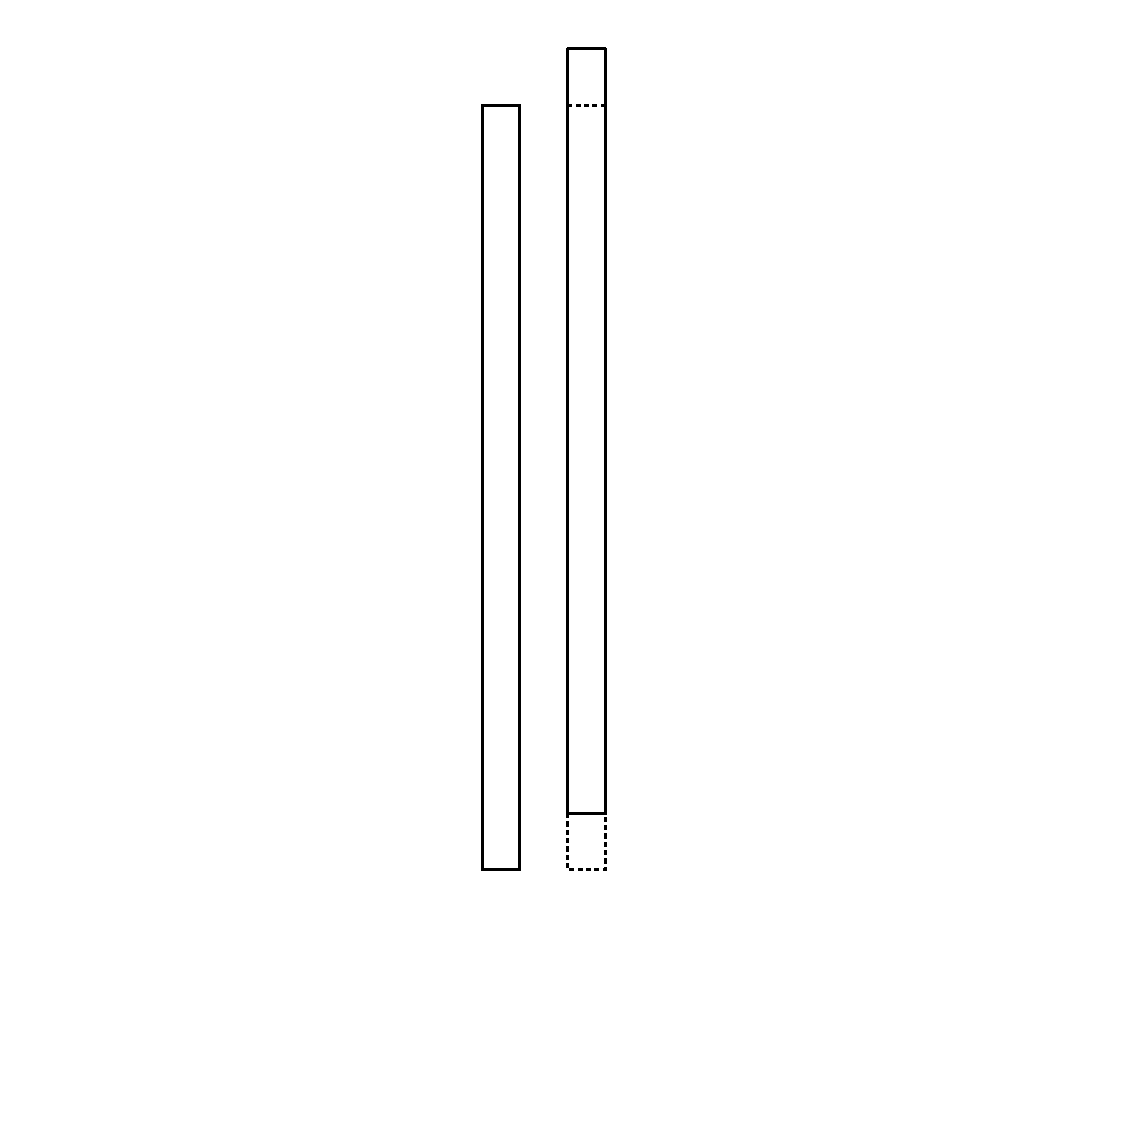
\includegraphics[trim=3.0cm 1.6cm 2.0cm 0.8cm, clip=true, width=0.19\textwidth]{algorithms-harvard/misal4.pdf}
	}
	\subfloat[b][Top half shift in $r$]{
		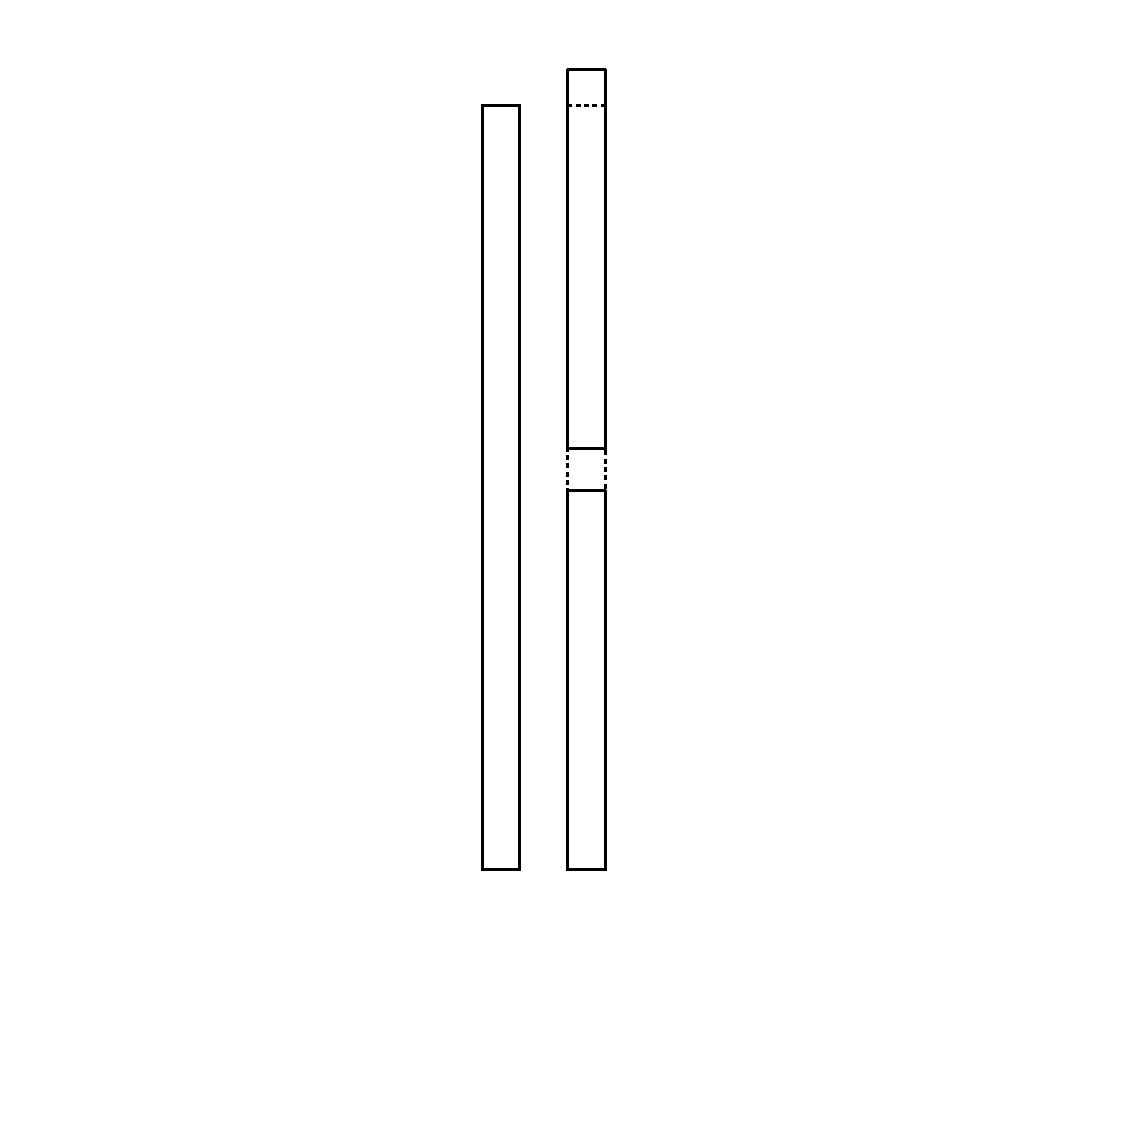
\includegraphics[trim=3.0cm 1.6cm 2.0cm 0.8cm, clip=true, width=0.19\textwidth]{algorithms-harvard/misal5.pdf}
	}
	\subfloat[c][$\phi$ rotation]{
		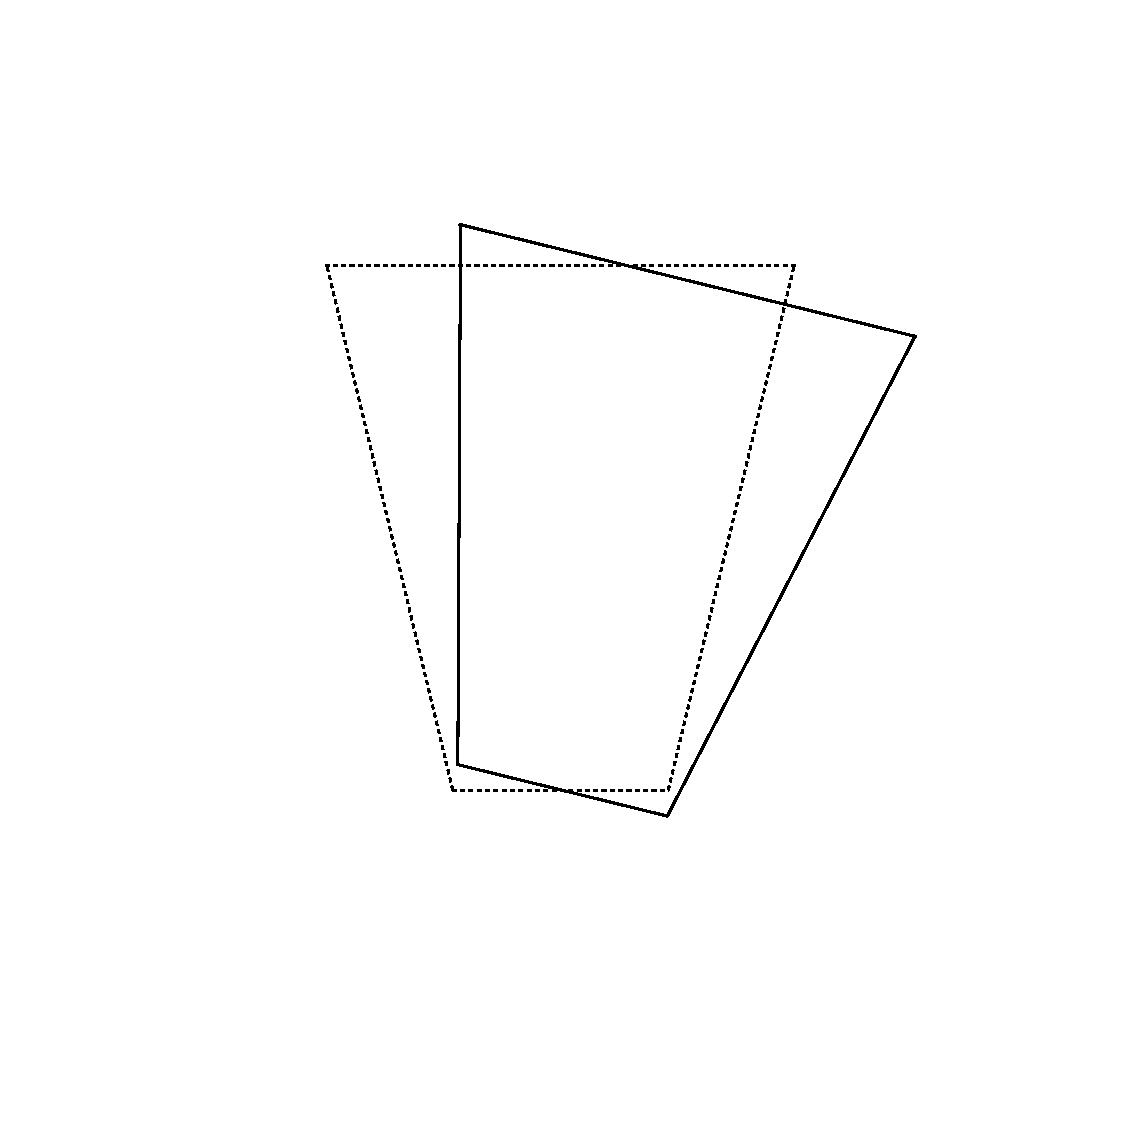
\includegraphics[trim=3.0cm 1.6cm 2.0cm 0.8cm, clip=true, width=0.19\textwidth]{algorithms-harvard/misal2.pdf}
	}
	\subfloat[d][$\theta_{\rm tilt}$]{
		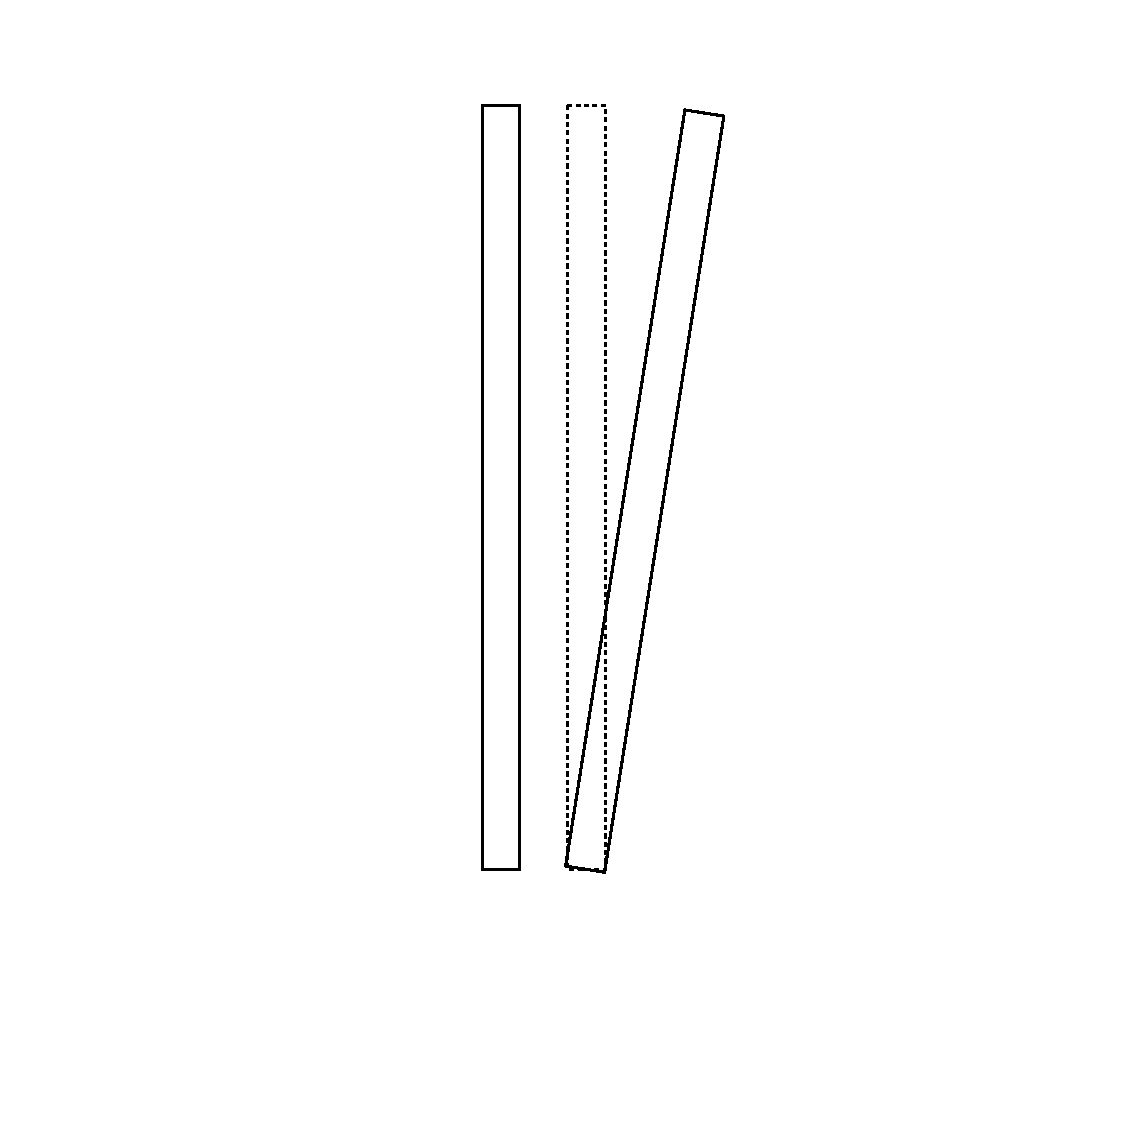
\includegraphics[trim=3.0cm 1.6cm 2.0cm 0.8cm, clip=true, width=0.19\textwidth]{algorithms-harvard/misal3.pdf}
	}
	\subfloat[e][Shift in $z$]{
		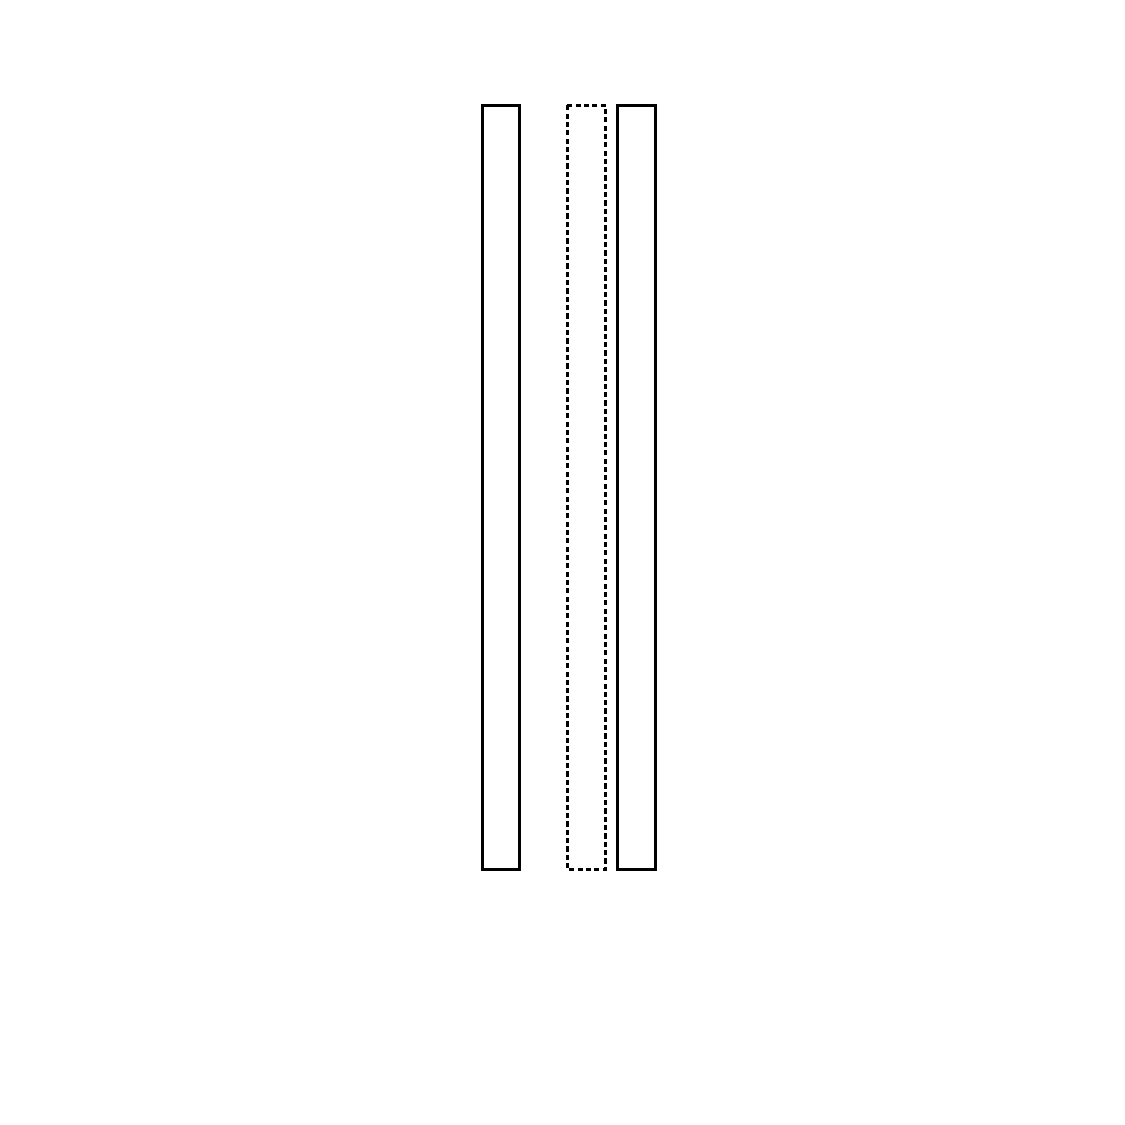
\includegraphics[trim=3.0cm 1.6cm 2.0cm 0.8cm, clip=true, width=0.19\textwidth]{algorithms-harvard/misal1.pdf}
	}

	\caption{\label{fig:harvard_misal_illustration}
	Illustration of the position of the different multiplets in the different misalignment configurations
	considered in this section. In all cases except (c), the IP is to the left and the image shows
	the $r$-$z$ plane passing through the center of the wedge. In (c), the $r$-$\phi$ plane is shown
	as it would look from the IP.
	}
	\end{center}
\end{figure}

These misalignments are simulated through the use of true hits in the Athena simulation.
The true hit position that causes the trigger to fire is known. It is thus trivial to overlay a
misaligned geometry over the true hits and recalculate the strips that were hit. Misalignments
corresponding to up to 5\,mm shifts in the relative positions of the two wedges are considered.
For the $\phi$ rotations and the $\theta_{\rm tilt}$ this corresponds to up to $1.36$\,mrad.

The performance of the trigger algorithm is studied with and without misalignments. In addition,
corrections have been implemented for all cases illustrated in Figure\,\ref{fig:harvard_misal_illustration}
except case (c). The implementation of the corrections happens in steps\,A and~E of the algorithm, described
in Section\,\ref{sec:harvard_impl}, without any additional resource overhead.
In particular, as already detailed, $2\times 8\times 16$ constants, corresponding
to 8 planes and 16 MMFEs, store the radial offset and $z$ position of the corresponding strips. These constants
can be updated to perfectly counteract the effects of the cases illustrated above in (a), (b) and (e). Case
(d) can also be corrected with some loss of accuracy, since only 16 $z$ positions are stored along the tilted
plane. The $z$ positions stored can be optimized, but for the studies in this document the middle $z$ position
of the strips read out by each MMFE is used. The loss of accuracy from this simplified corrections is quantified
in the next section. Corrections for case (c) have not been studied yet, but the effects of such a misalignment
have been studied and are shown in the next section.

%%%%%%%%%%%%%%%%%%%%%%%%%%%%%%%%%%%
\subsubsubsection{Performance}
\label{sec:harv-perf}

The performance of the algorithm is studied using single muon events generated with Athena
full simulation. A geometry with two equal quadruplets each with two horizontal strips and two
different-tilt stereo strips (xxuv) was used. Most of the studies used here use a geometry
in which the quadruplets are placed with horizontal strips placed closer to the IP
(xxuv xxuv).

The samples were generated using muons generated at the IP. However, additional
samples with typical parameters of the ATLAS beamspot during Run\,1
using for the origin of the muons Gaussian distributions of mean $(x,y,z)=(0.05,0.06,-1)$\,mm
and $(\sigma_x,\sigma_y,\sigma_z)=(0.01,0.01,70)$\,mm have also been checked. The
results with the samples with realistic beamspot (not shown here) result in a degradation of
the $\theta$ resolution of about a factor of two, but no noticeable effects on the $\Delta\theta$
or $\phi$ resolutions or the trigger efficiency.
Two samples using
muons with energies of 200 and 1000\,\GeV have been studied. Each sample has 20000 events
with muons pointing to one large sector of the NSW.
Of the digitized hits found in the simulation, the first
registered signal per channel was chosen for trigger construction.
A function mimicking a VMM chip's 100\,ns deadtime and coverage of
64 strips was also applied to the data.  This function serves to guarantee a
maximum of one hit, true or background, is registered for each 64 grouping of strips for each event.

Three set of studies complement the performance studies in ideal conditions:
\begin{itemize}\itemsep-4pt
\item a study of the effects of incoherent background,
\item a study of the impact of misalignments and the corrections designed to mitigate them,
\item a study of the performance with quadruplets with mirror-image placement (xxuv uvxx), proposed recently
to increase the lever-arm for fitting the bending coordinate using horizontal (x) strips.
\end{itemize}

The following variables are used to parameterize performance. Fit efficiency is defined as the efficiency
for a track to trigger the detector given that a minimum number of trigger hits before including background exist.
In particular, n-horizontal/n-stereo refers to events for which there were at least n hits in the horizontal strips and
the same amount in the stereo strips before addition of background hits. Distributions are calculated with respect
to truth definitions. In particular, the distributions of $\theta^{\rm{fit}}-\theta^{\rm{true}}$,
$\phi^{\rm{fit}}-\phi^{\rm{true}}$, and $\Delta\theta^{\rm{fit}}-\Delta\theta^{\rm{true}}$, for which true coordinates and direction
are defined at the entrance of the NSW, are studied. The distributions are fit using Gaussian fits with a one-step recursive
fit. The raw results are first fitted to a gaussian. The quoted resolutions are obtained through a fit in the range
$[\mu_1-3\sigma_1,\mu_1+3\sigma_1]$, where $\mu_1$ and $\sigma_1$ are the mean and standard deviation of the first fit. Tails
are defined as the fraction of events outside the range $[\mu_1-3\sigma_1,\mu_1+3\sigma_1]$.

Sample distributions, integrated over all $\eta$, are shown for the $\phi$, $\theta$ and $\Delta\theta$ reconstruction
in Figures\,\ref{fig:phi_harvard}, \ref{fig:theta_harvard} and \ref{fig:dtheta_harvard}.
\begin{figure}[htbp]
	\centering
%	\subfloat[a][]{
%		\includegraphics[width=0.33\textwidth]{algorithms-harvard/50GeVphi_etaall.pdf}
%	}
	\subfloat[a][]{
		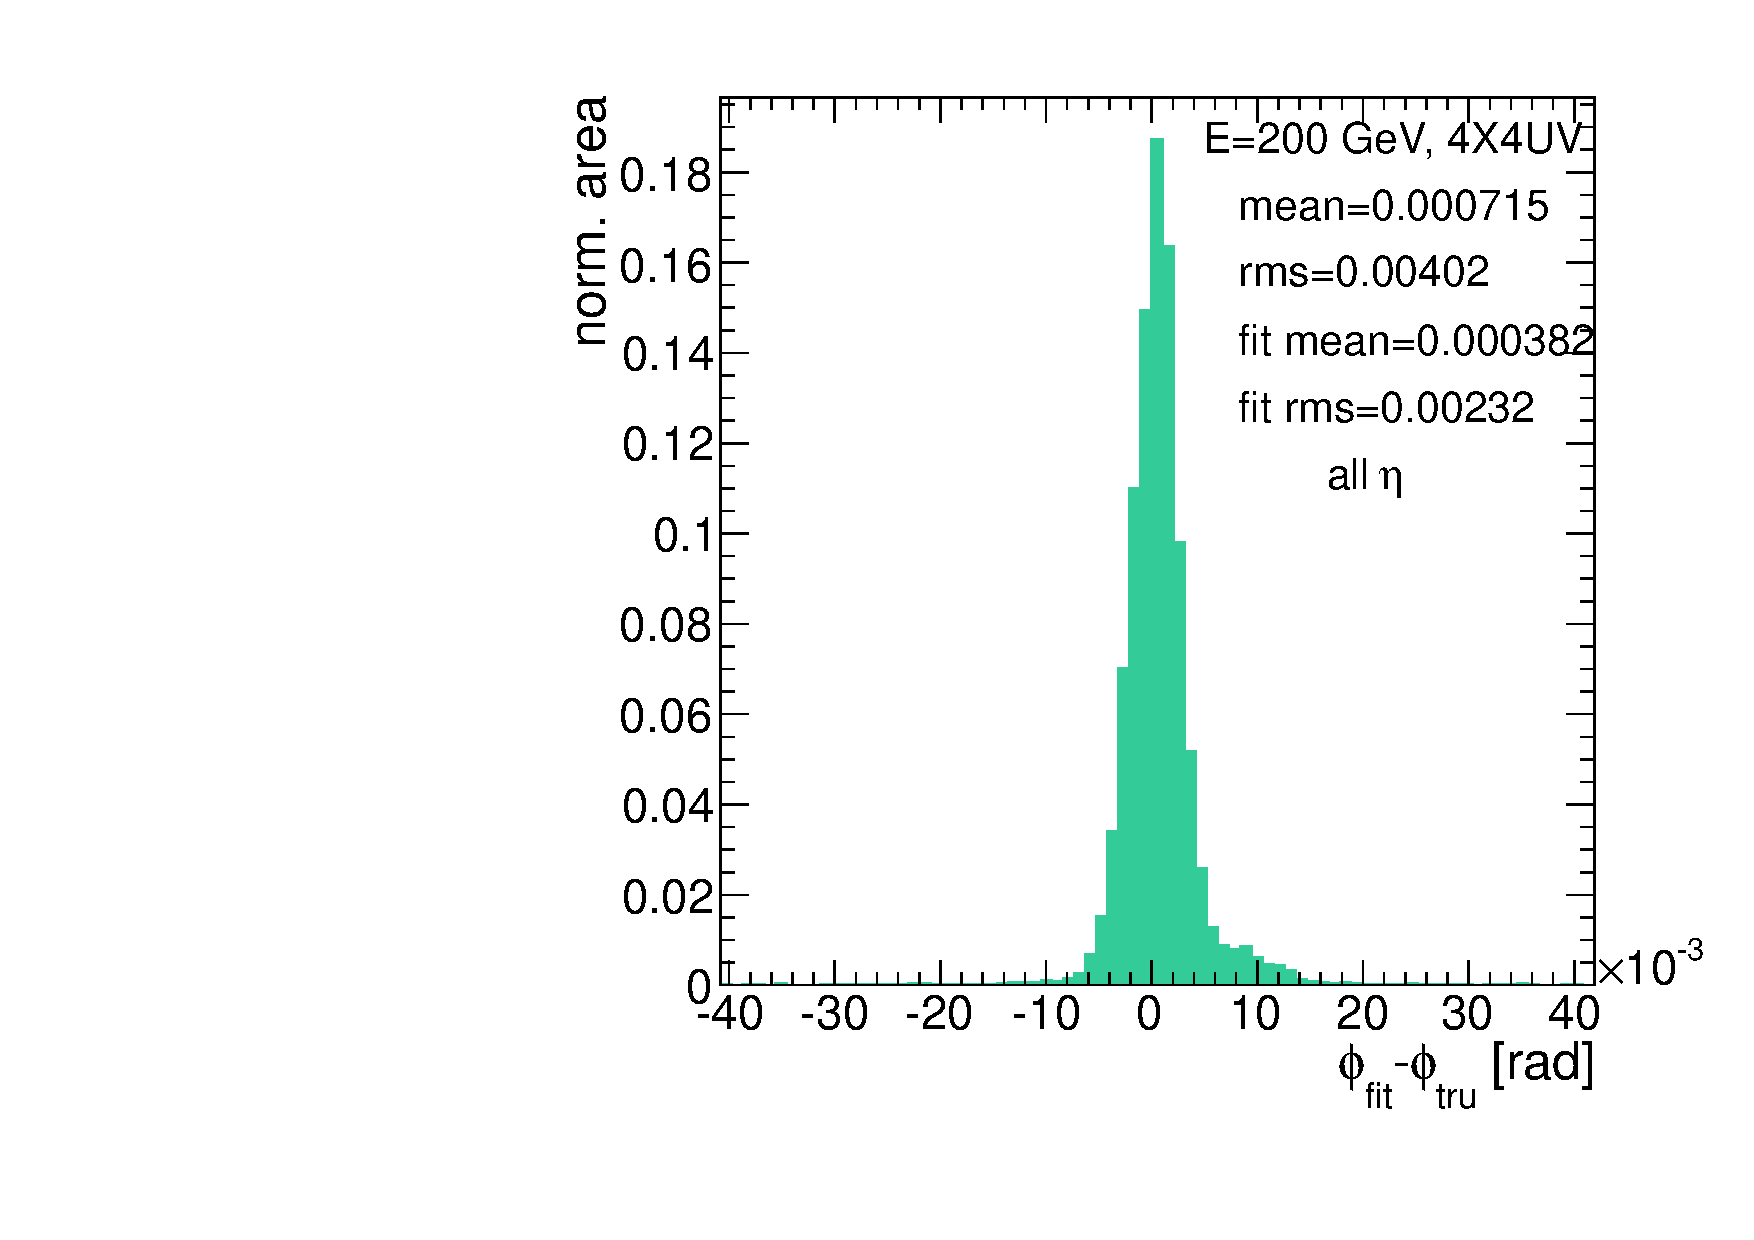
\includegraphics[width=0.4\textwidth]{algorithms-harvard/200GeVphi_etaall.pdf}
	}
	\subfloat[b][]{
		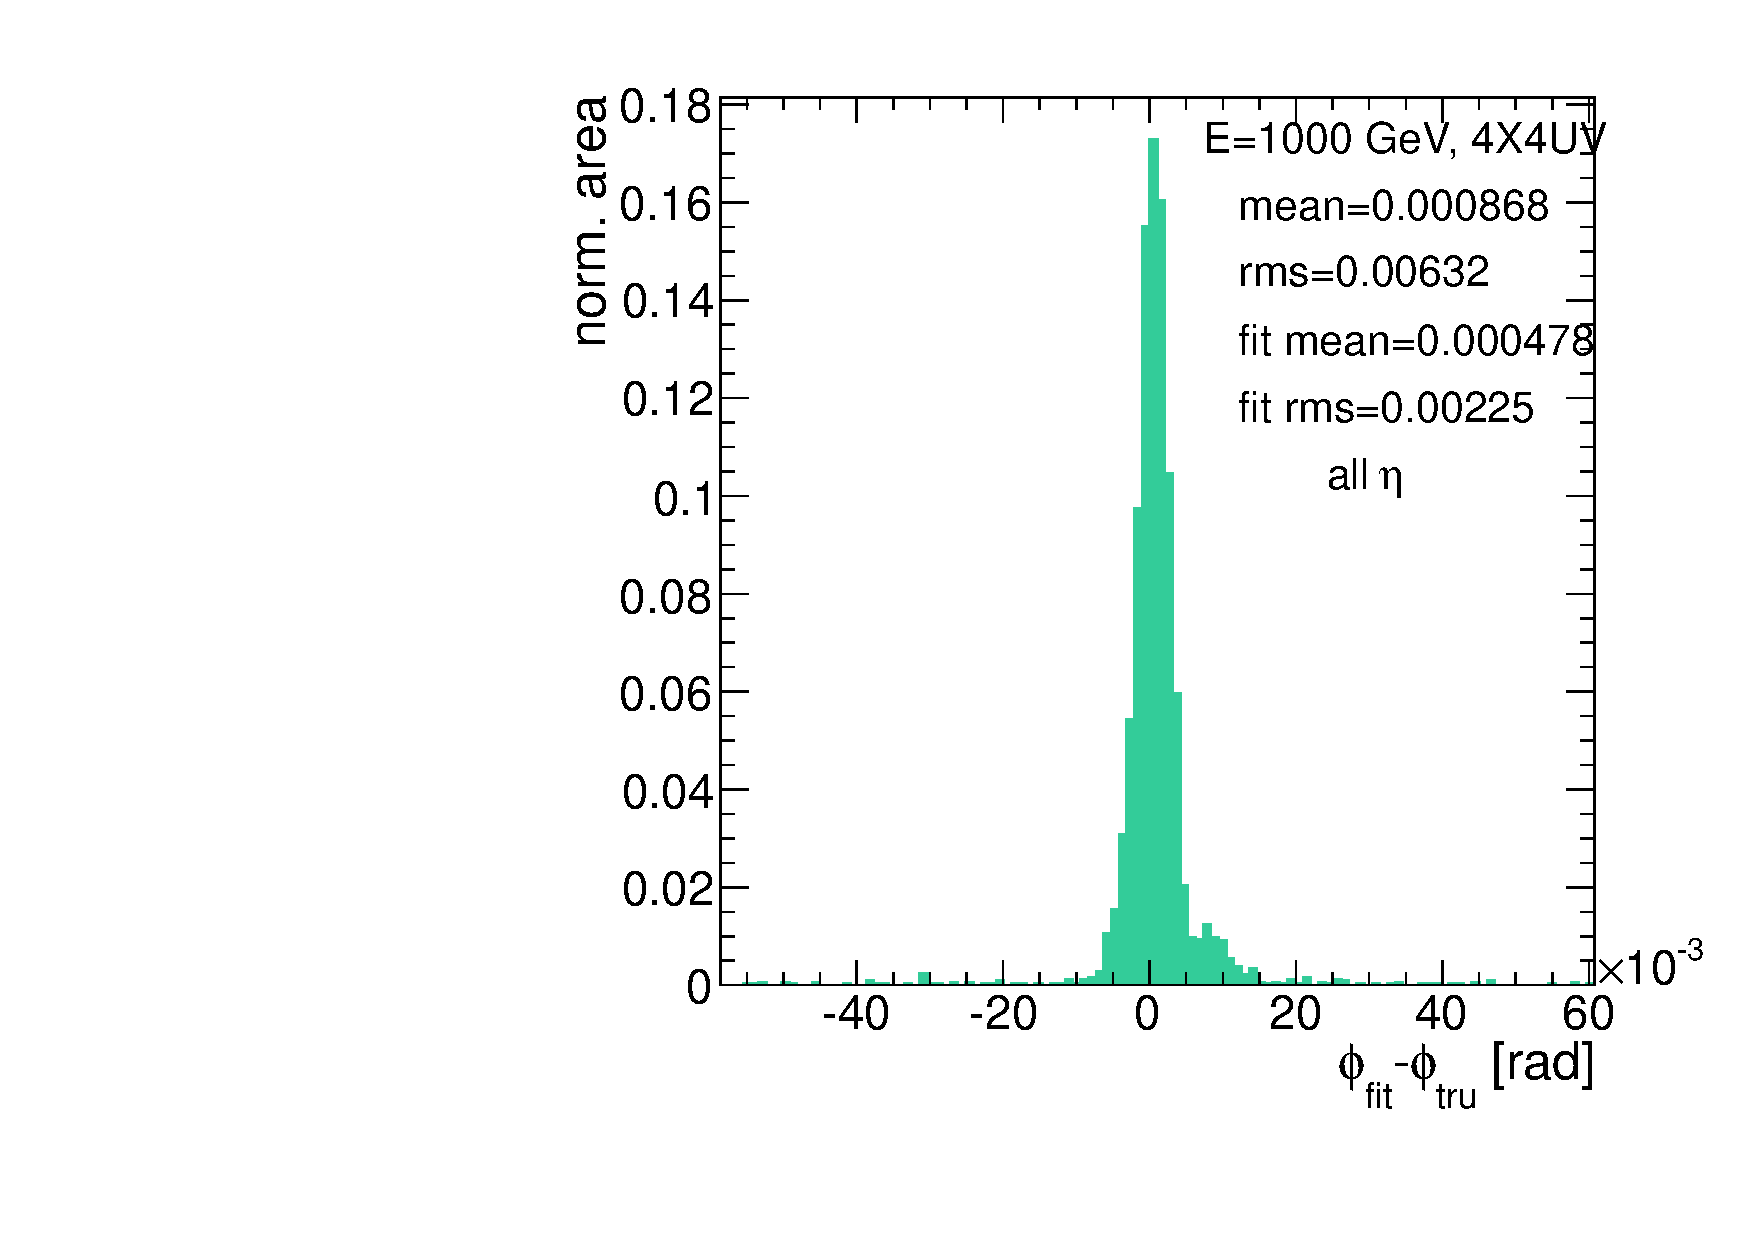
\includegraphics[width=0.4\textwidth]{algorithms-harvard/1000GeVphi_etaall.pdf}
	}\\
	\caption{\label{fig:phi_harvard}
Distribution of reconstructed $\phi$ minus true $\phi$ value of the track at the entrance of the NSW
for muons of $E=200\GeV$ (a) and $E=1\TeV$ (b). The xxuv xxuv configuration without background
is used.
	}
\end{figure}

\begin{figure}[htbp]
	\centering
%	\subfloat[a][]{
%		\includegraphics[width=0.33\textwidth]{algorithms-harvard/50GeVtheta_etaall.pdf}
%	}
	\subfloat[a][]{
		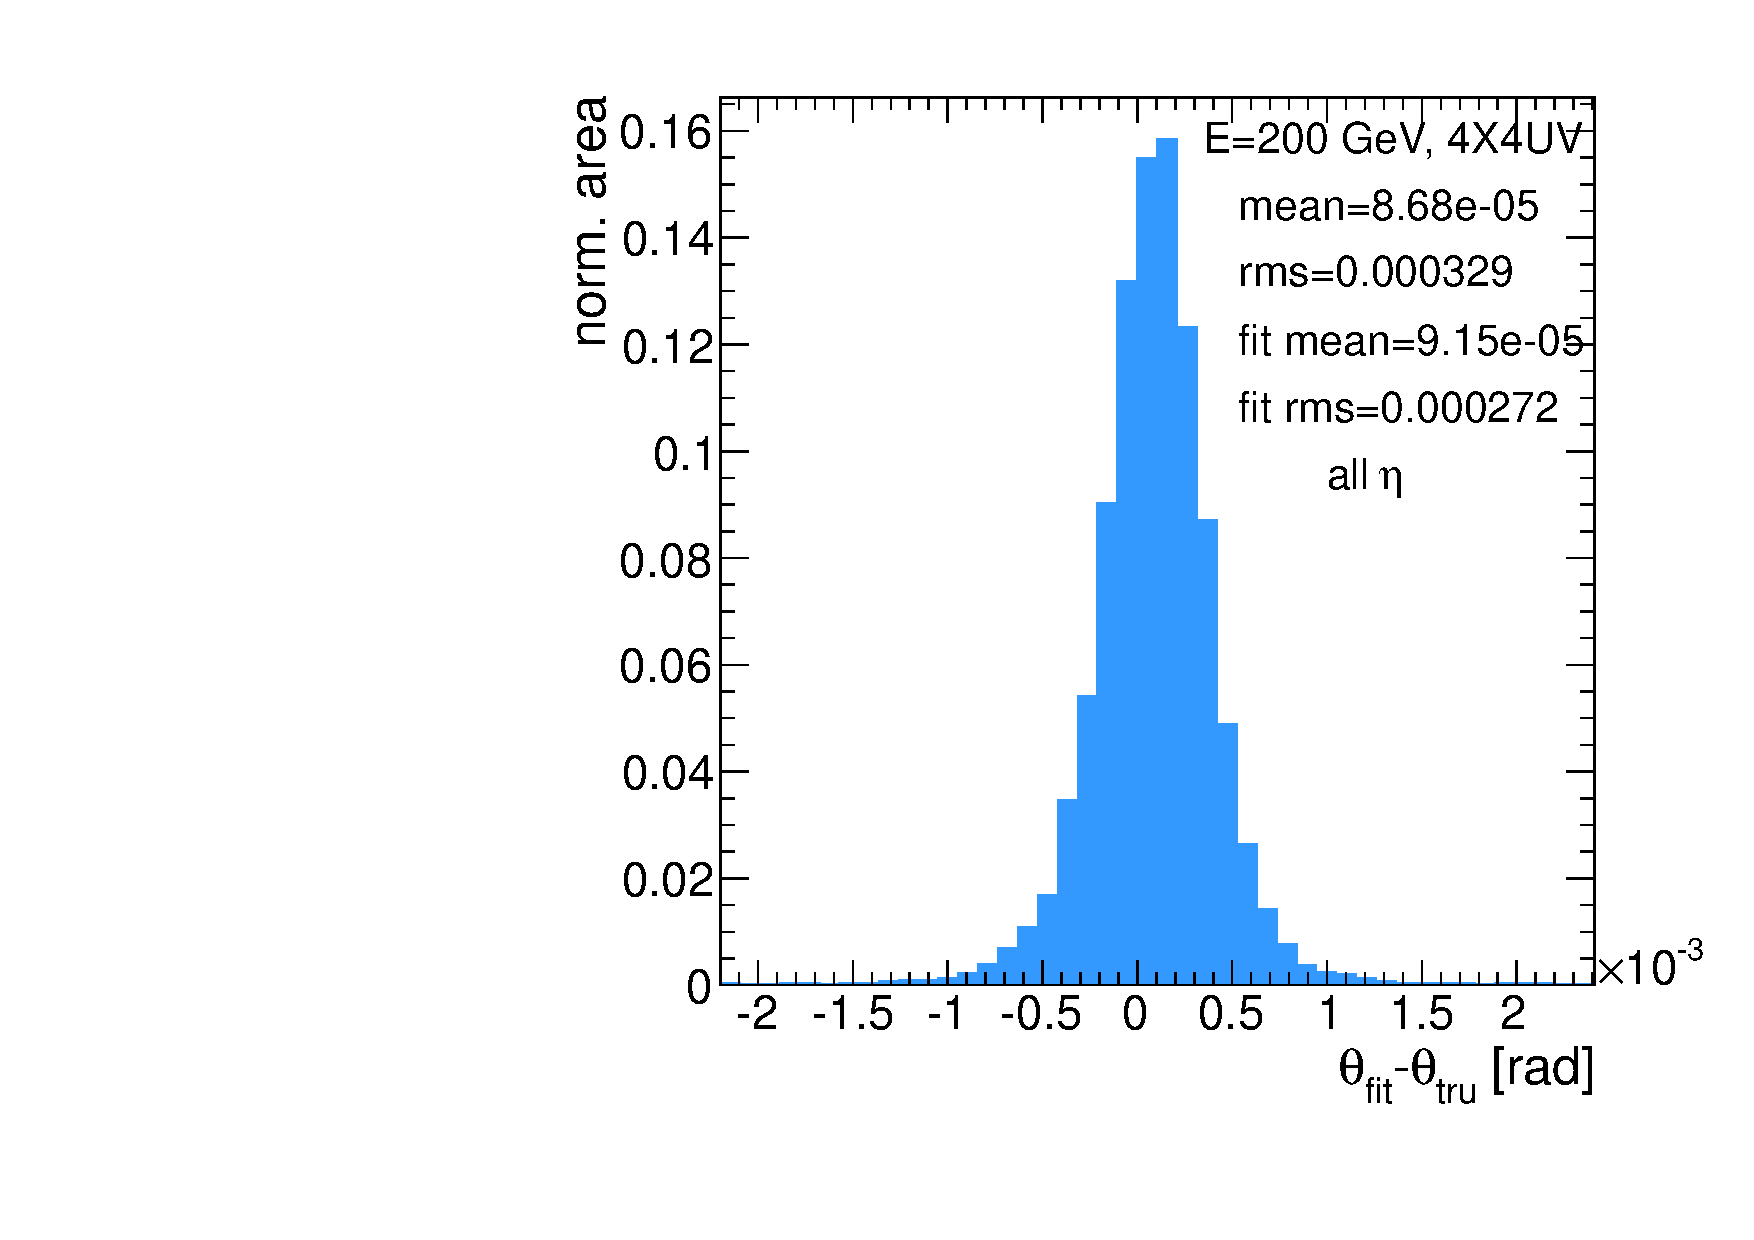
\includegraphics[width=0.45\textwidth]{algorithms-harvard/200GeVtheta_etaall.pdf}
	}
	\subfloat[b][]{
		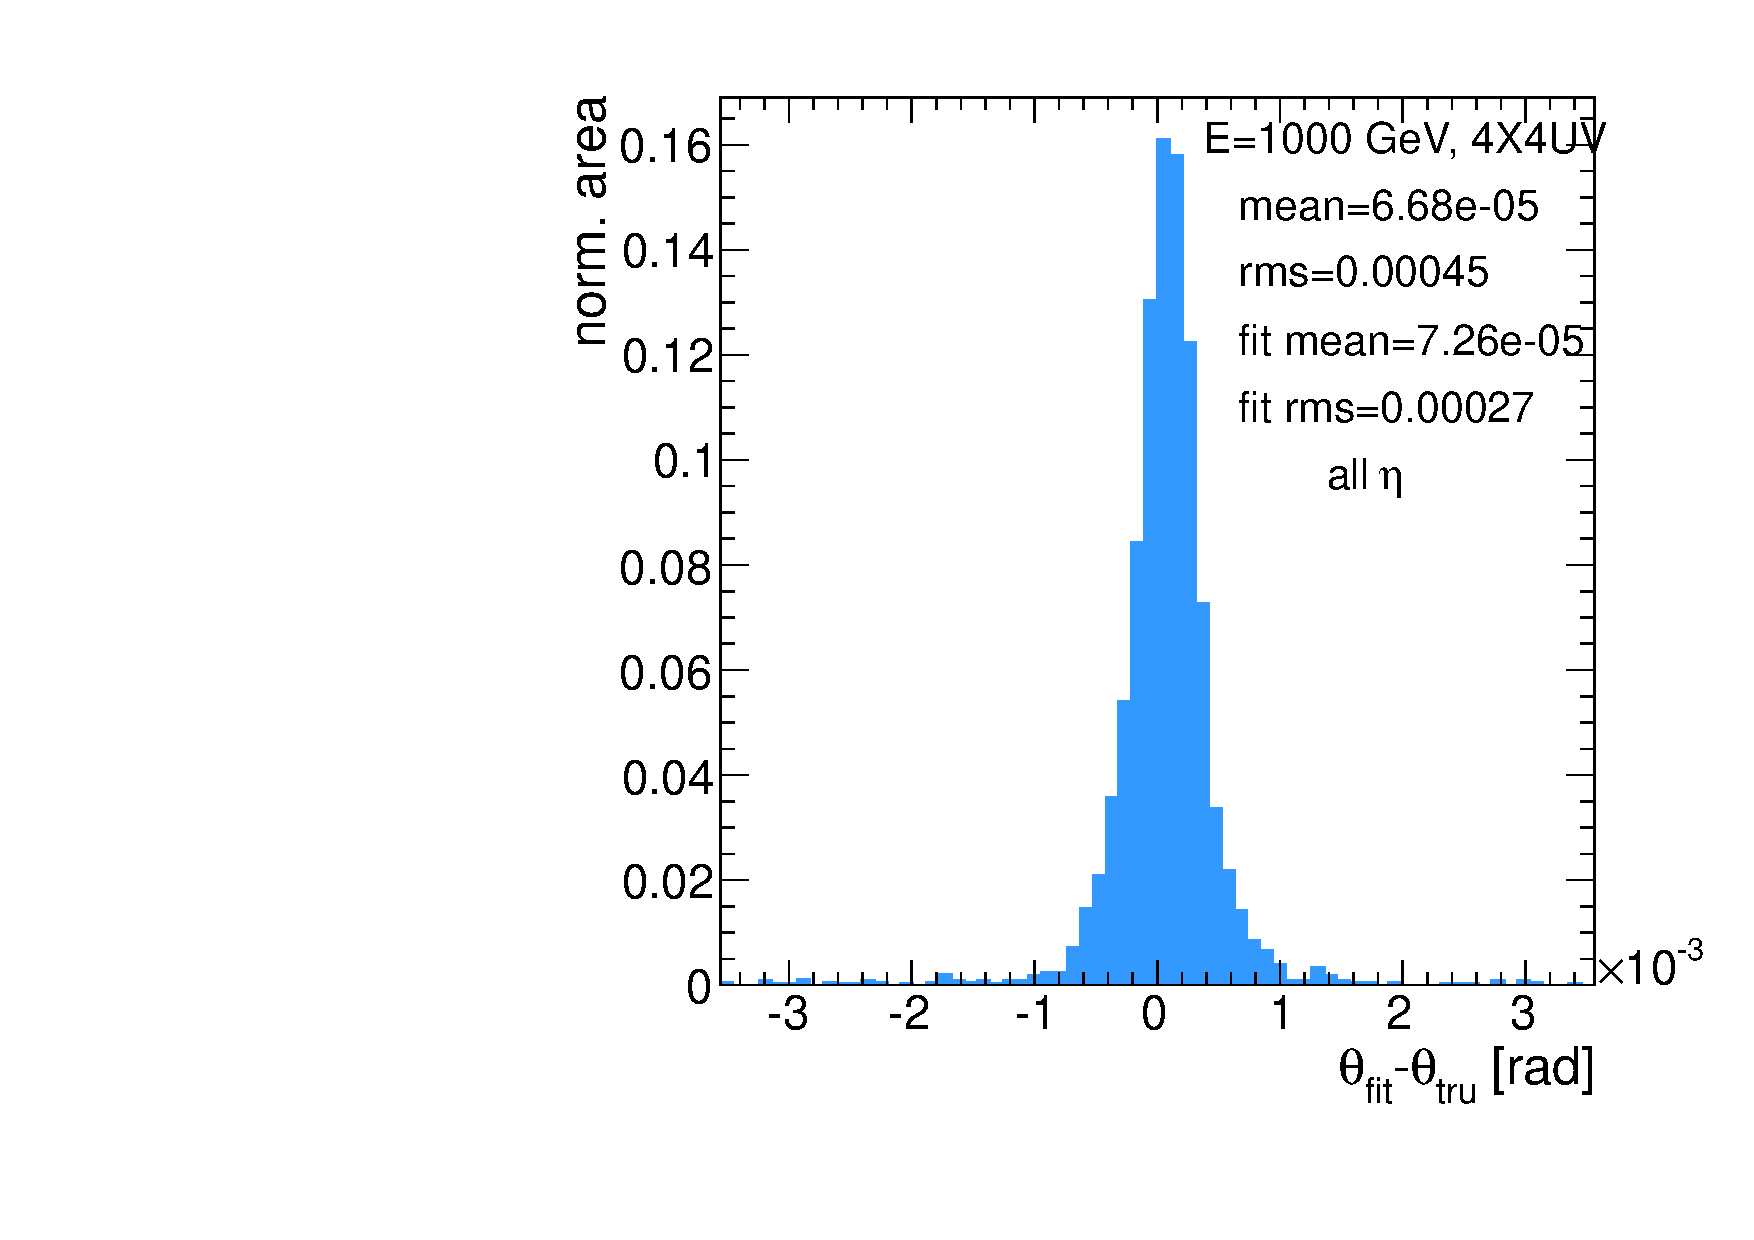
\includegraphics[width=0.45\textwidth]{algorithms-harvard/1000GeVtheta_etaall.pdf}
	}\\
	\caption{\label{fig:theta_harvard}
Distribution of reconstructed global $\theta$ minus true global $\theta$ value of the track at the entrance of the NSW
for muons of $E=200\GeV$ (a) and $E=1\TeV$ (b). The xxuv xxuv configuration without background
is used.
	}
\end{figure}

\begin{figure}[htbp]
	\centering
%	\subfloat[a][]{
%		\includegraphics[width=0.33\textwidth]{algorithms-harvard/50GeVdtheta_etaall.pdf}
%	}
	\subfloat[a][]{
		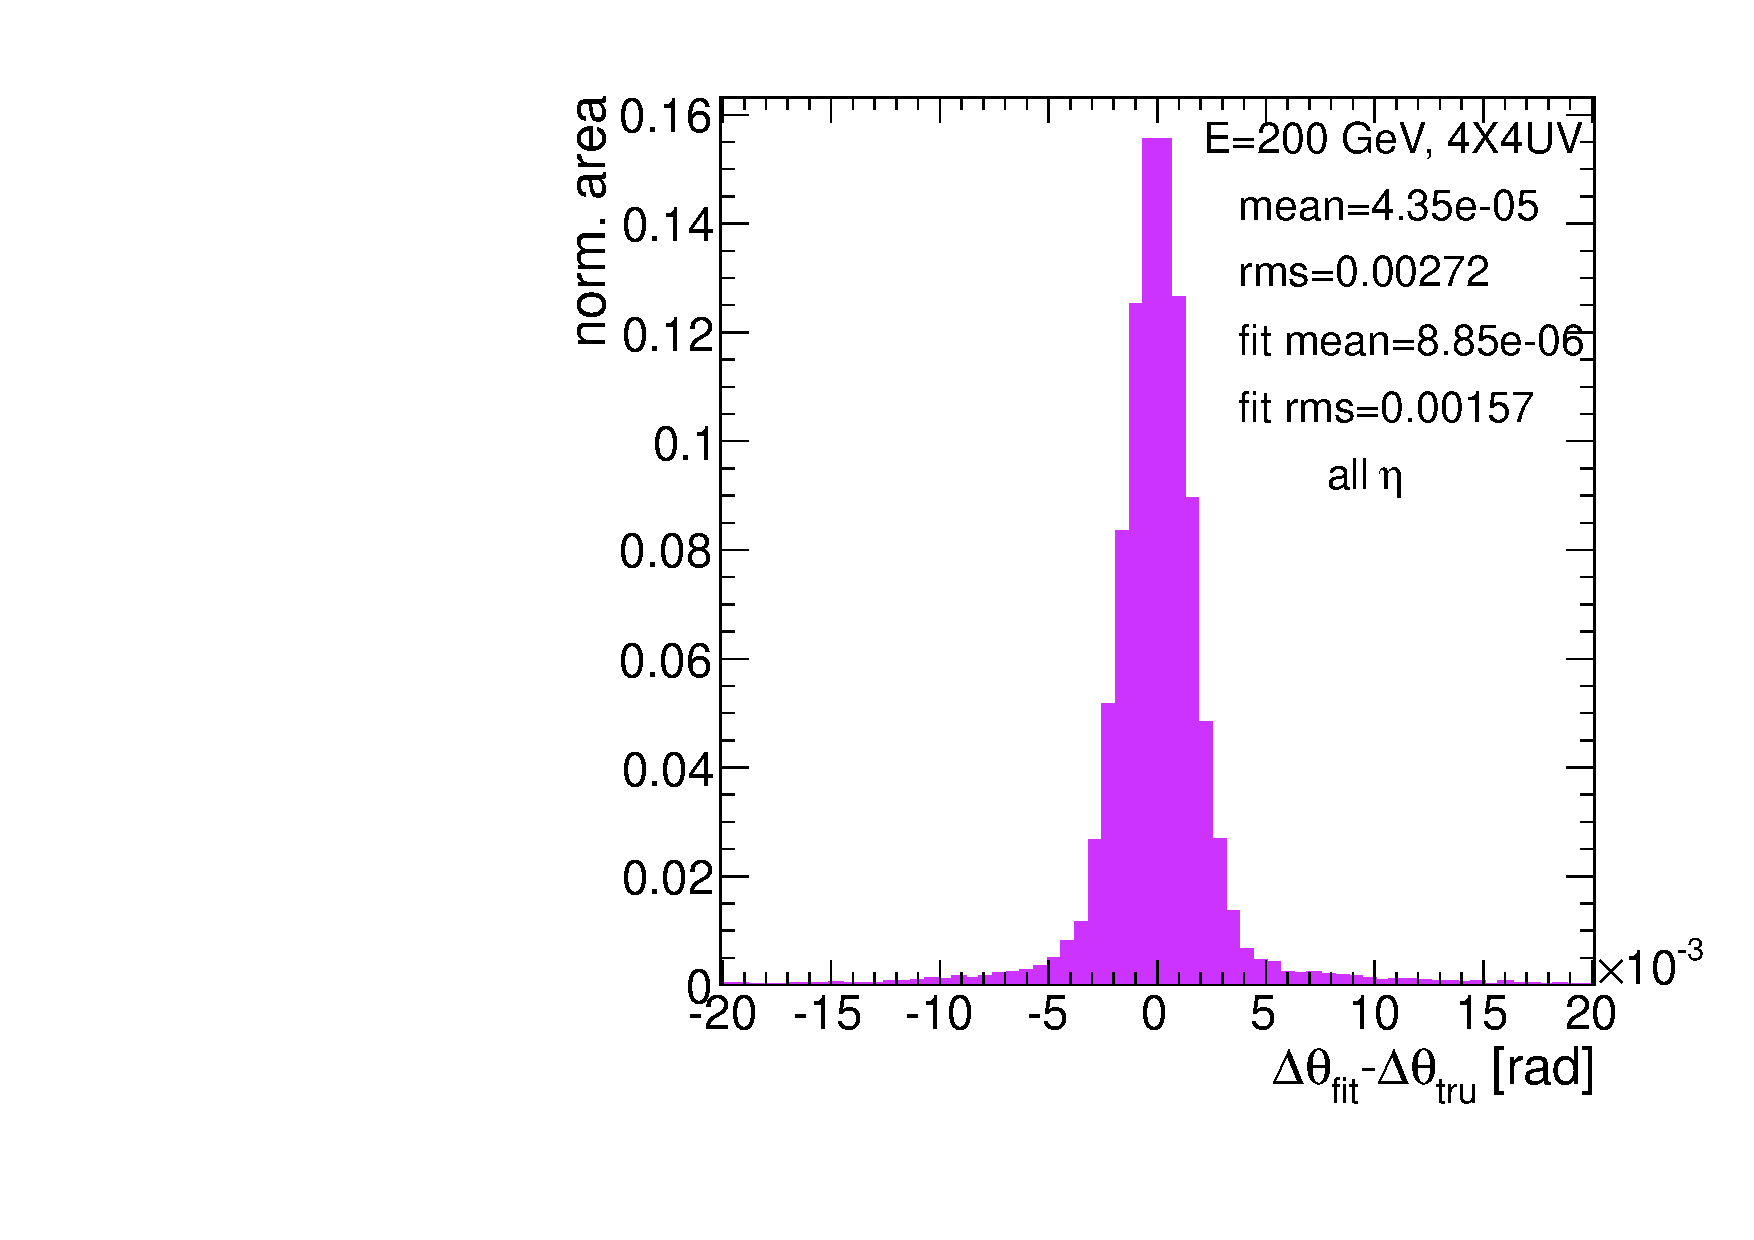
\includegraphics[width=0.45\textwidth]{algorithms-harvard/200GeVdtheta_etaall.pdf}
	}
	\subfloat[b][]{
		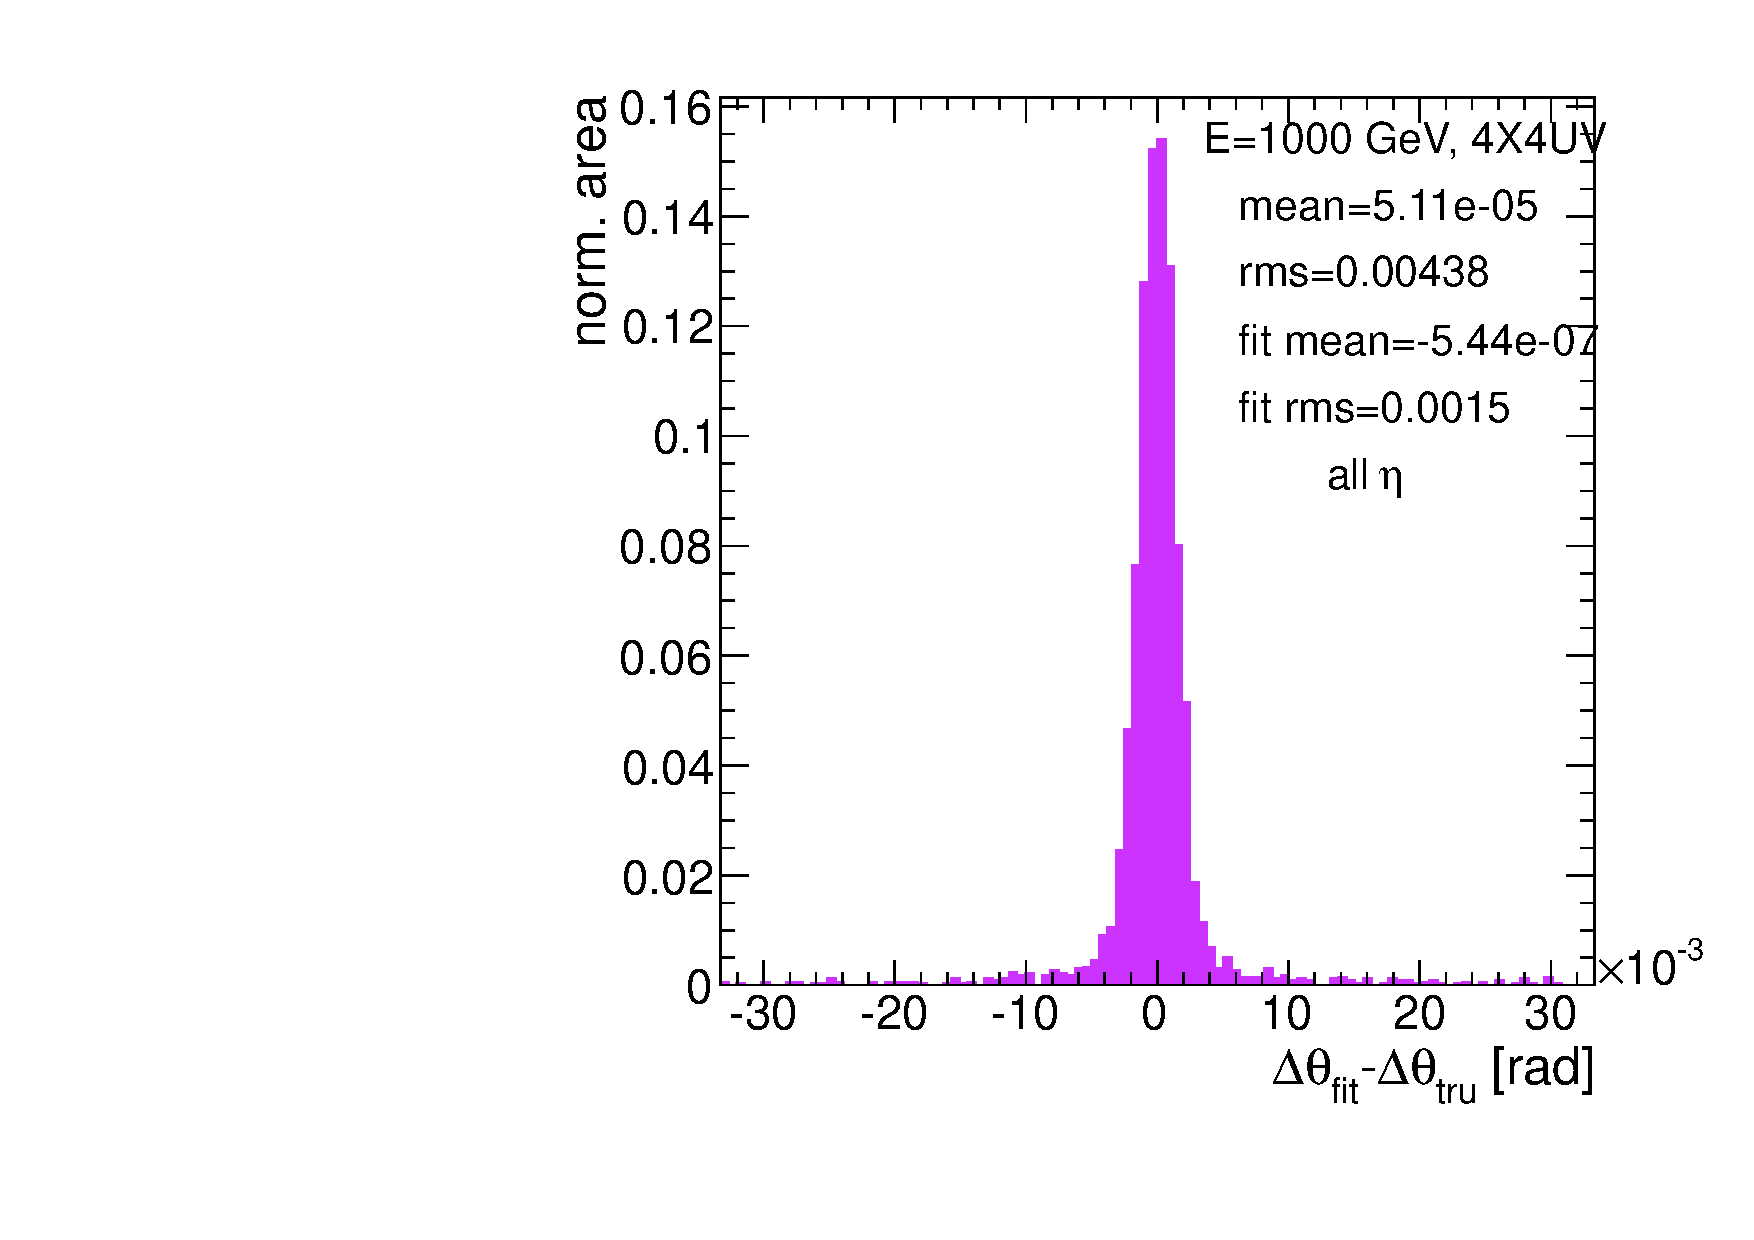
\includegraphics[width=0.45\textwidth]{algorithms-harvard/1000GeVdtheta_etaall.pdf}
	}\\
	\caption{\label{fig:dtheta_harvard}
Distribution of reconstructed $\Delta\theta$ minus true $\Delta\theta$ value of the track at the entrance of the NSW
for muons of $E=200\GeV$ (a) and $E=1\TeV$ (b). The xxuv xxuv configuration without background
is used.
	}
\end{figure}

The distributions do not change significantly with energy, except for an increase in the tails for the highest
energy studied. This is caused by an increase in events with large number of secondary particles,
which throw off the fit when they occur.

Figure~\ref{fig:harvard_ideal_eff}~(a) shows the efficiency of the algorithm for events for which
truth hits are found for different thresholds. The $E=200\GeV$ sample and an ideal geometry
without background is used. The efficiency increases with the number of hits as expected because
of the extra redundancy added by the additional hits, which makes the fit more likely to succeed
even if some hits are not usable. The efficiency of the algorithm is very close to 100\%.
Figure~\ref{fig:harvard_ideal_eff}~(b) shows the true efficiency of each category, where the denominator
includes all muons at the entrance of the spectrometer. In this case the x-axis should be interpreted as
an inclusive axis (the 2X, 1U or 1V case refers to tracks with at least that many hits, so it includes all
events falling in the other bins). This figure thus includes the algorithmic efficiency in Figure~\ref{fig:harvard_ideal_eff}~(a)
and the detector efficiency. It also gives a quantitative answer about the fraction of tracks with a given
number of coincidence threshold requirements. Finally, Figure~\ref{fig:harvard_ideal_eff}~(c) shows the efficiency with the
same definition as was used in Figure~\ref{fig:SaclayEfficiencyForDifferentPairRequirement} for easy comparison. It should
be noted that the minimum fit requirement in Figure~\ref{fig:harvard_ideal_eff}~(c) is two horizontal strips and one stereo
strip. This is a rather loose requirement, so it should be no surprise that the efficiencies are higher than for Figure~\ref{fig:SaclayEfficiencyForDifferentPairRequirement}. However, tighter requirements can also be observed in the
figure as the x axis increases.
\begin{figure}[htbp]
	\centering
	\subfloat[a][]{
		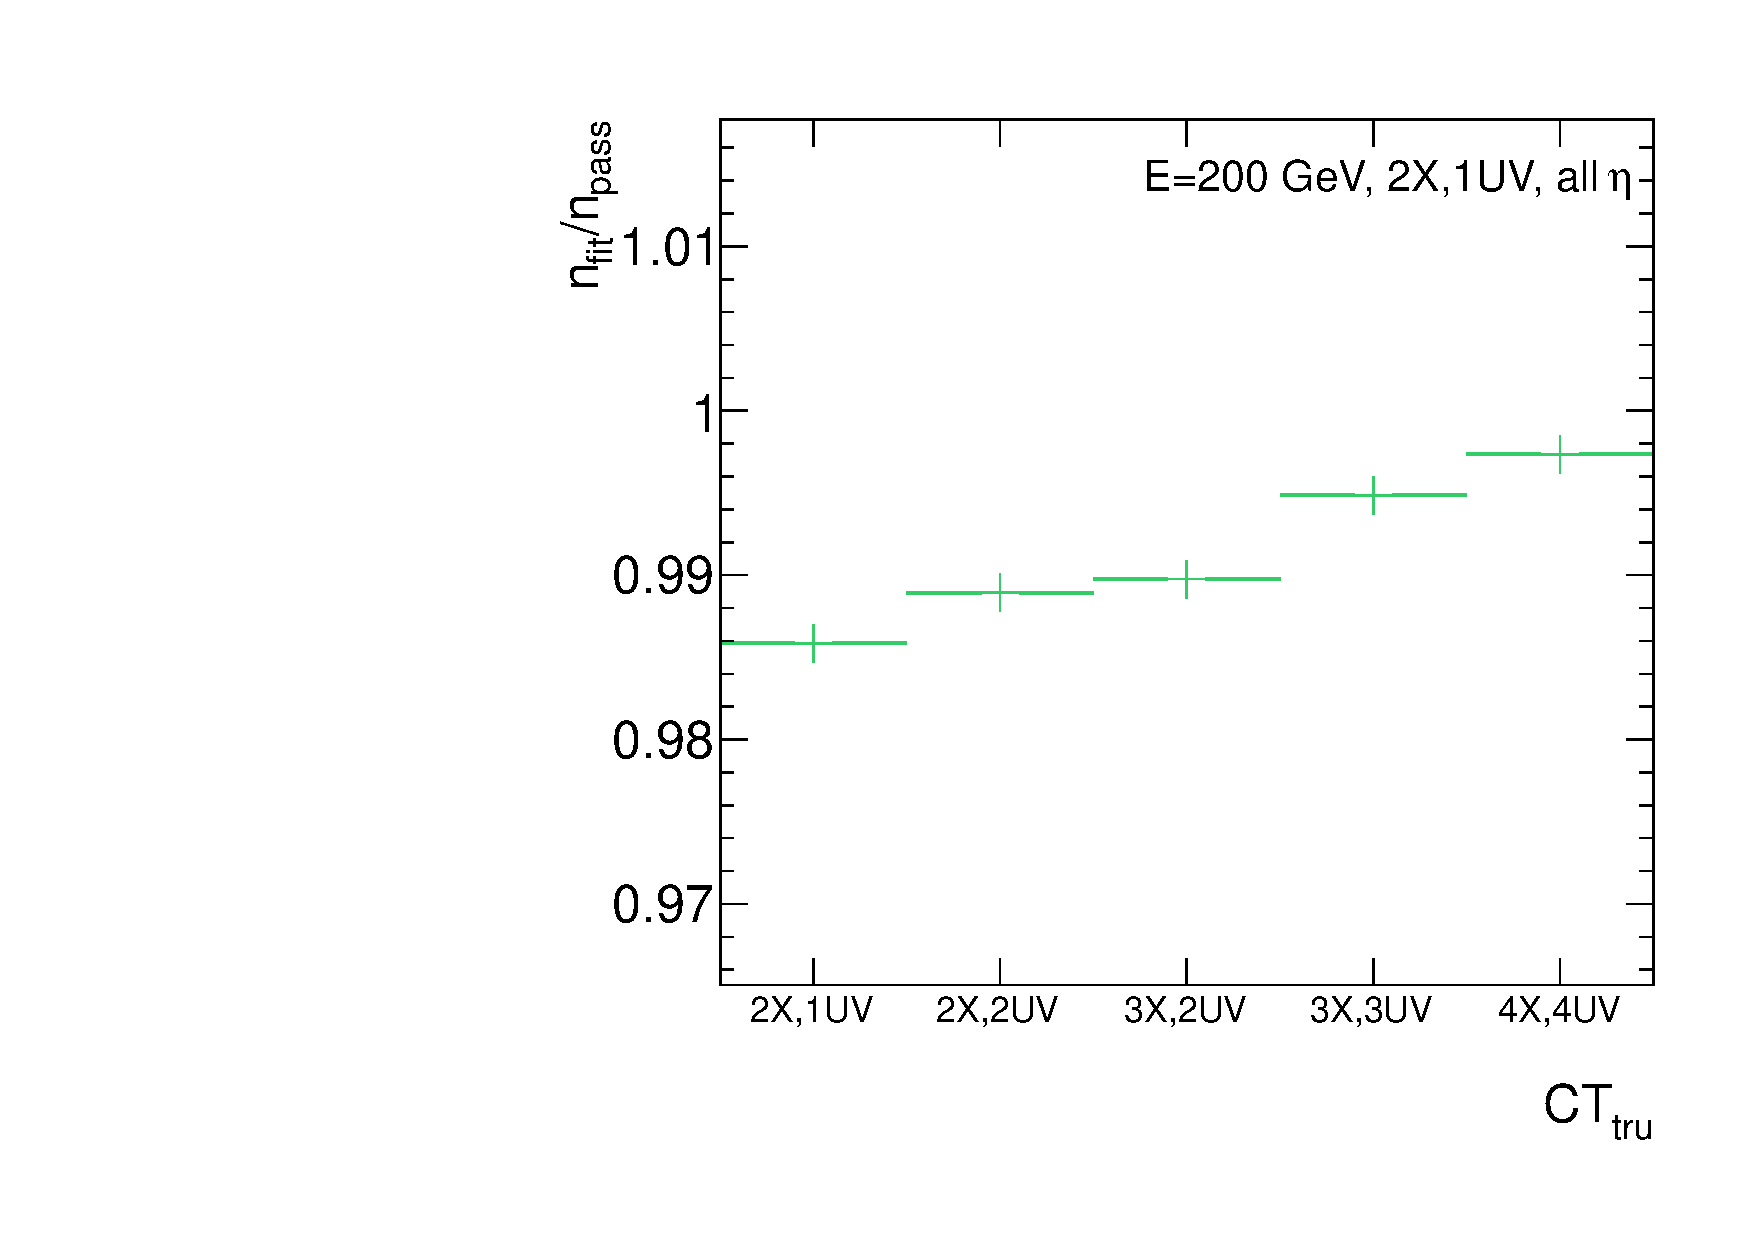
\includegraphics[width=0.33\textwidth]{algorithms-harvard/ct_var_2x_1uv_etaall_eff_note_200GeV.pdf}
	}
	\subfloat[b][]{
		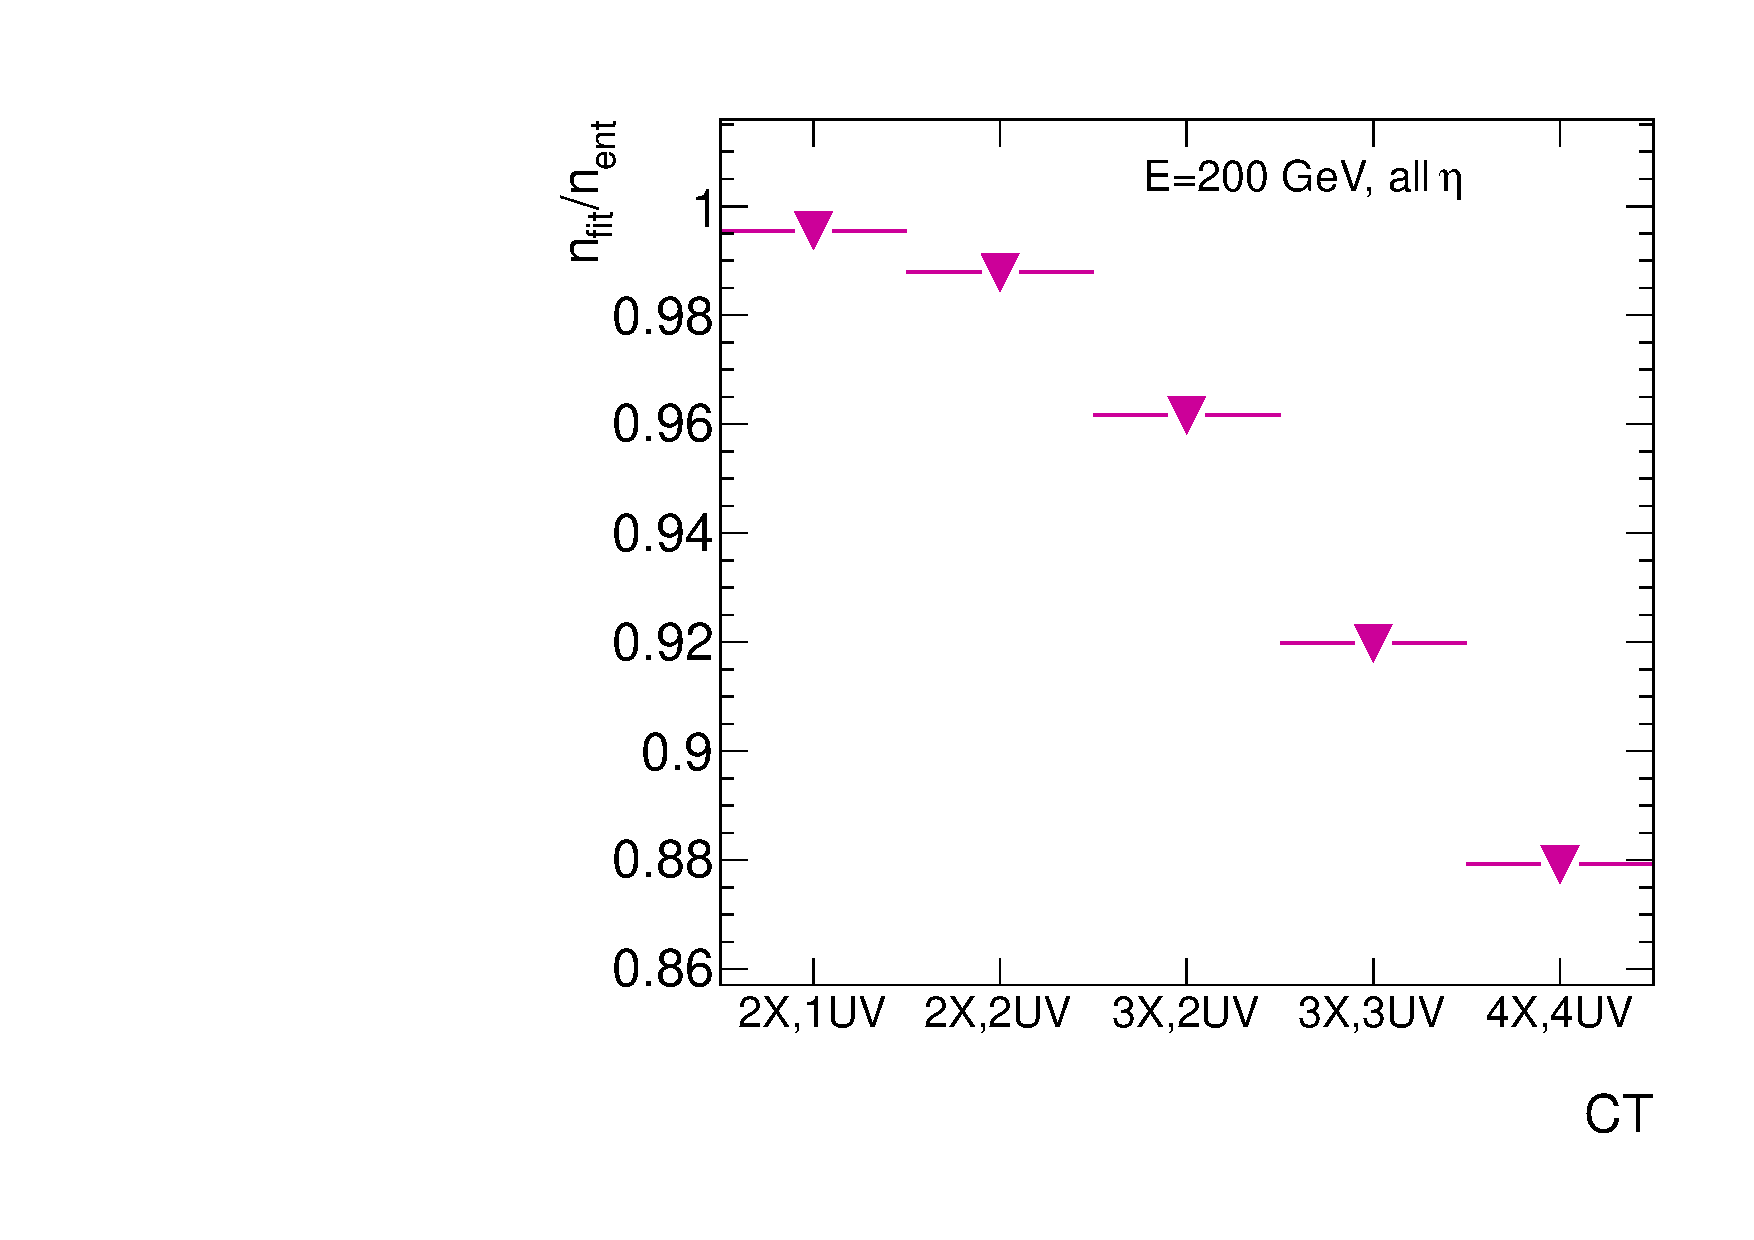
\includegraphics[width=0.33\textwidth]{algorithms-harvard/ct_var_etaall_eff_tru_200GeV.pdf}
	}
	\subfloat[c][]{
	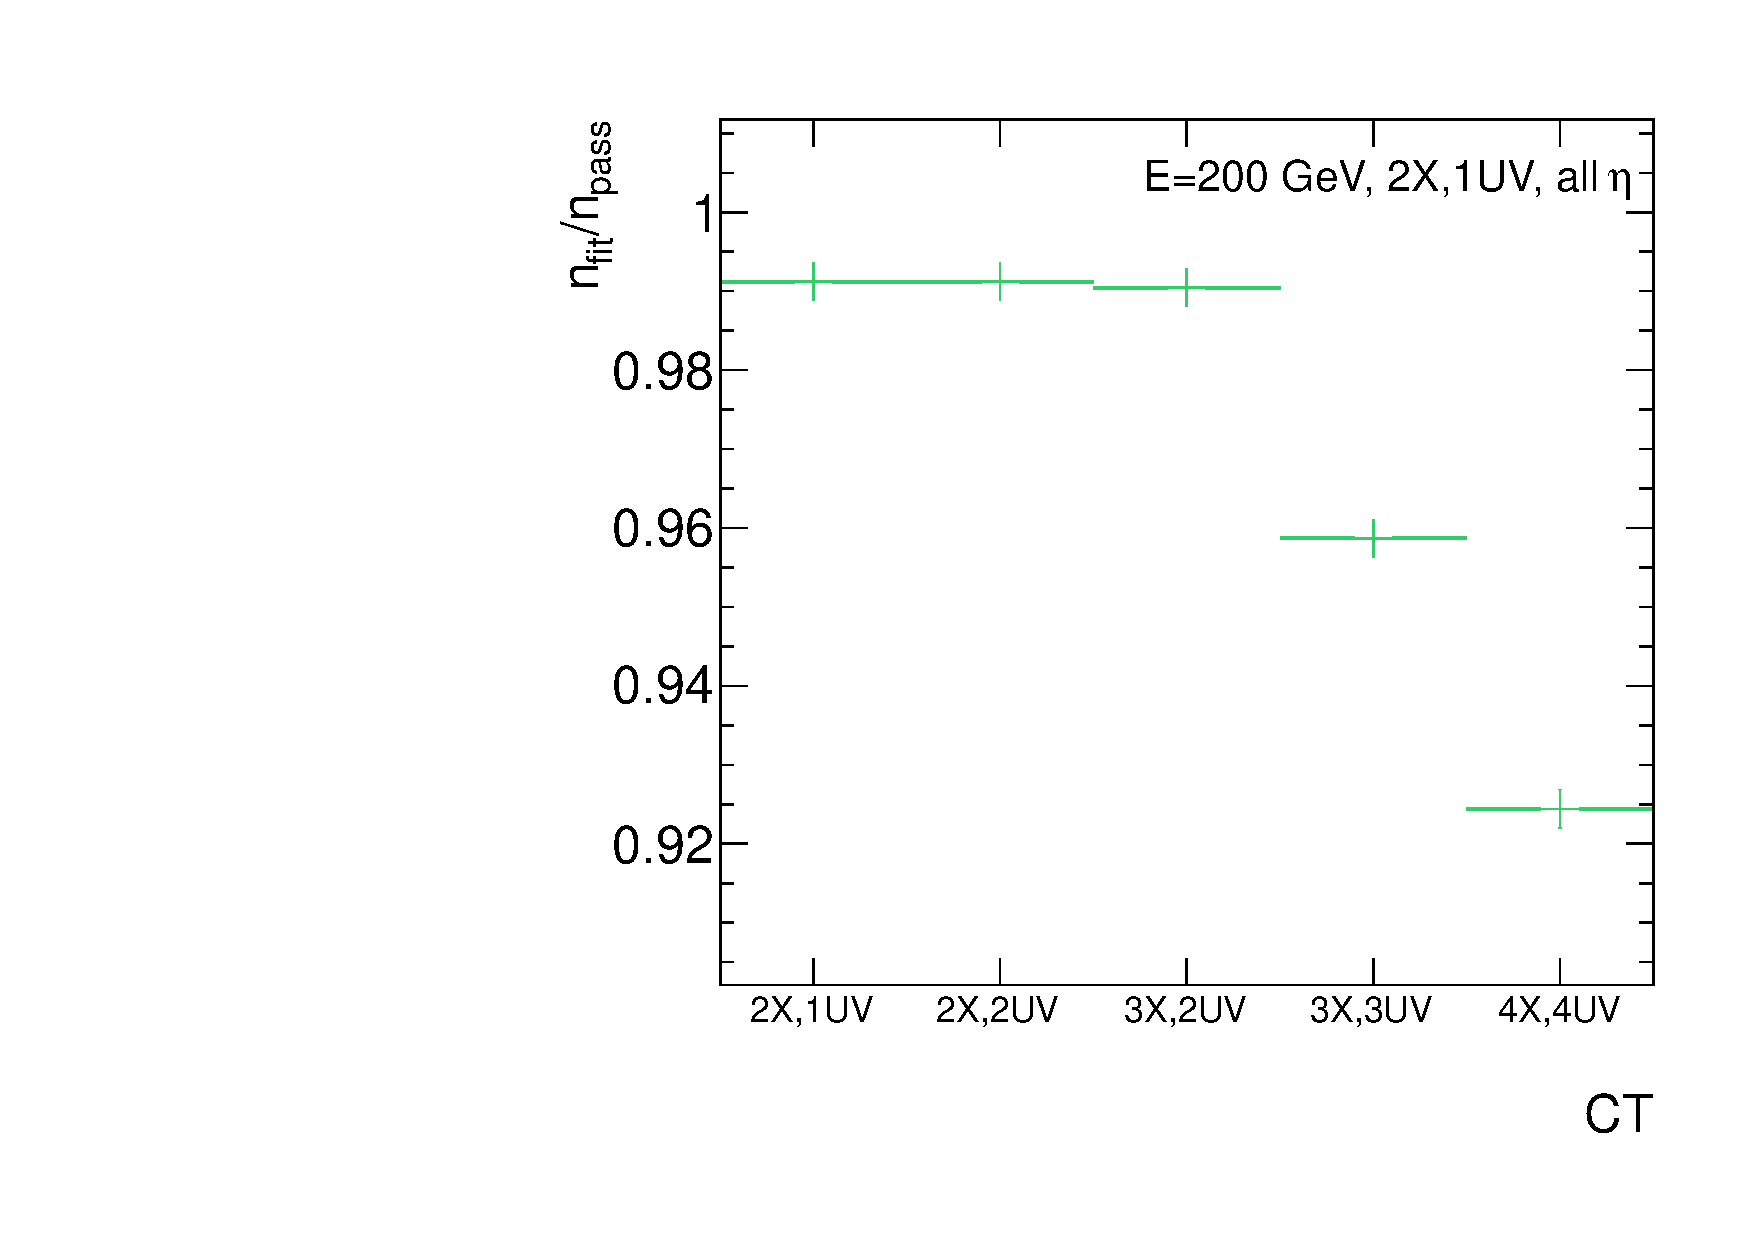
\includegraphics[width=0.33\textwidth]{algorithms-harvard/ct_var_2x_1uv_etaall_eff_6hit_200GeV.pdf}
	}
	\caption{\label{fig:harvard_ideal_eff}
Algorithmic efficiency~(a) showing for different coincidence thresholds (CT) at the truth trigger digit level,
the fraction of tracks that are fit. Total efficiency~(b) showing for different coincidence thresholds at the reconstructed
level, the fraction of total muons incident in the NSW surface that are fit with those thresholds. The efficiency for
different thresholds given that at least six hits are found at the truth level, as defined in Figure~\ref{fig:SaclayEfficiencyForDifferentPairRequirement} are shown in~(c).
	}
\end{figure}


The $\phi^{\rm{fit}}$, $\theta^{\rm{fit}}$ and $\Delta\theta^{\rm{fit}}$ resolutions for the ideal geometry for $E=200\GeV$ muons
without backgrounds, obtained from a fit are summarized in Table\,\ref{tab:efficiencyHarvardIdeal}. The efficiency, defined
as for Figure~\ref{fig:harvard_ideal_eff} (a) is also shown. 

\begin{table}[htbp]
\caption{Efficiency and resolution (mrad) for muons of $E=200\GeV$ for different coincidence thresholds without background.
\label{tab:efficiencyHarvardIdeal}  }
\centering
\begin{tabular}{l l c c c c}
\toprule
Track Type & Fit Efficiency & $\sigma(\theta^{\rm{fit}})$ (tails) & $\sigma(\phi^{\rm{fit}})$ (tails) & $\sigma(\Delta\theta^{\rm{fit}})$ (tails) \\ [0.5ex]
\midrule
4-horizontal/4-stereo & 99.8\% & 0.27 (0.83\%) & 2.3 (1.5\%) & 1.6 (0.65\%) \\
3-horizontal/3-stereo & 99.5\% & 0.28 (0.89\%) & 3.0 (0.97\%) & 1.7 (0.47\%)   \\
2-horizontal/2-stereo & 99.0\% & 0.29 (0.97\%) & 3.2 (1.1\%) & 1.9 (1.0\%)   \\
\bottomrule
\end{tabular}
\end{table}

\paragraph{Effects from incoherent background}  \hfill \\
The impact of backgrounds is studied in the geometry with perfect alignment.
Incoherent background extrapolated from measurements performed in Run\,1\cite{CERN-LHCC-2011-012}
is added outside of Athena to each generated event as hits after
the digitization step.  Background hits are uniformly distributed in $\phi$, and in time across two bunch
crossings (50\,ns).  Once generated for each event, the background hits are combined with true event hits and a VMM-mimicking
function is called by the simulation to choose only the earliest arrival hit for each VMM chip, which allows for the background to
sometimes mask a true trigger hit.

The $\phi^{\rm{fit}}$, $\theta^{\rm{fit}}$ and $\Delta\theta^{\rm{fit}}$ resolutions for the ideal geometry for E\,=\,200\,GeV muons
with backgrounds are summarized in Table\,\ref{tab:efficiencyHarvardBkg}. The efficiency, defined
as for Figure~\ref{fig:harvard_ideal_eff} (a) is also shown. 

\begin{table}[htbp]
\caption{Efficiency and resolution (mrad) for muons of $E=200\GeV$ for different coincidence thresholds with background.
\label{tab:efficiencyHarvardBkg}  }
\centering
\begin{tabular}{l l c c c c}
\toprule
Track Type & Fit Efficiency & $\sigma(\theta^{\rm{fit}})$ (tails) & $\sigma(\phi^{\rm{fit}})$ (tails) & $\sigma(\Delta\theta^{\rm{fit}})$ (tails) \\ [0.5ex]
\midrule
4-horizontal/4-stereo & 99.3\% & 0.30 (1.4\%) & 4.2 (1.5\%) & 1.7 (0.37\%) \\
3-horizontal/3-stereo & 99.0\% & 0.31 (1.9\%) & 4.8 (2.1\%) & 2.0 (0.58\%)   \\
2-horizontal/2-stereo & 98.2\% & 0.32 (2.0\%) & 5.1 (2.2\%) & 2.3 (0.82\%)   \\
\bottomrule
\end{tabular}
\end{table}

\paragraph{Effects from misalignments within the NSW}  \hfill \\
For the misalignments studied in this section, no changes in efficiency or in the
resolution of $\theta$ and $\phi$ have been
observed. However, a degradation in the resolution of the $\Delta\theta$ reconstruction
has been observed.

Figure\,\ref{fig:harvard_misal_effect} shows the relative change in $\Delta\theta^{\rm{fit}}$ resolution as a function of misalignment
for the different misalignment configurations illustrated in Figure\,\ref{fig:harvard_misal_illustration}.

\begin{figure}[htbp]
	\centering
	\subfloat[a][Shift in $r$]{
		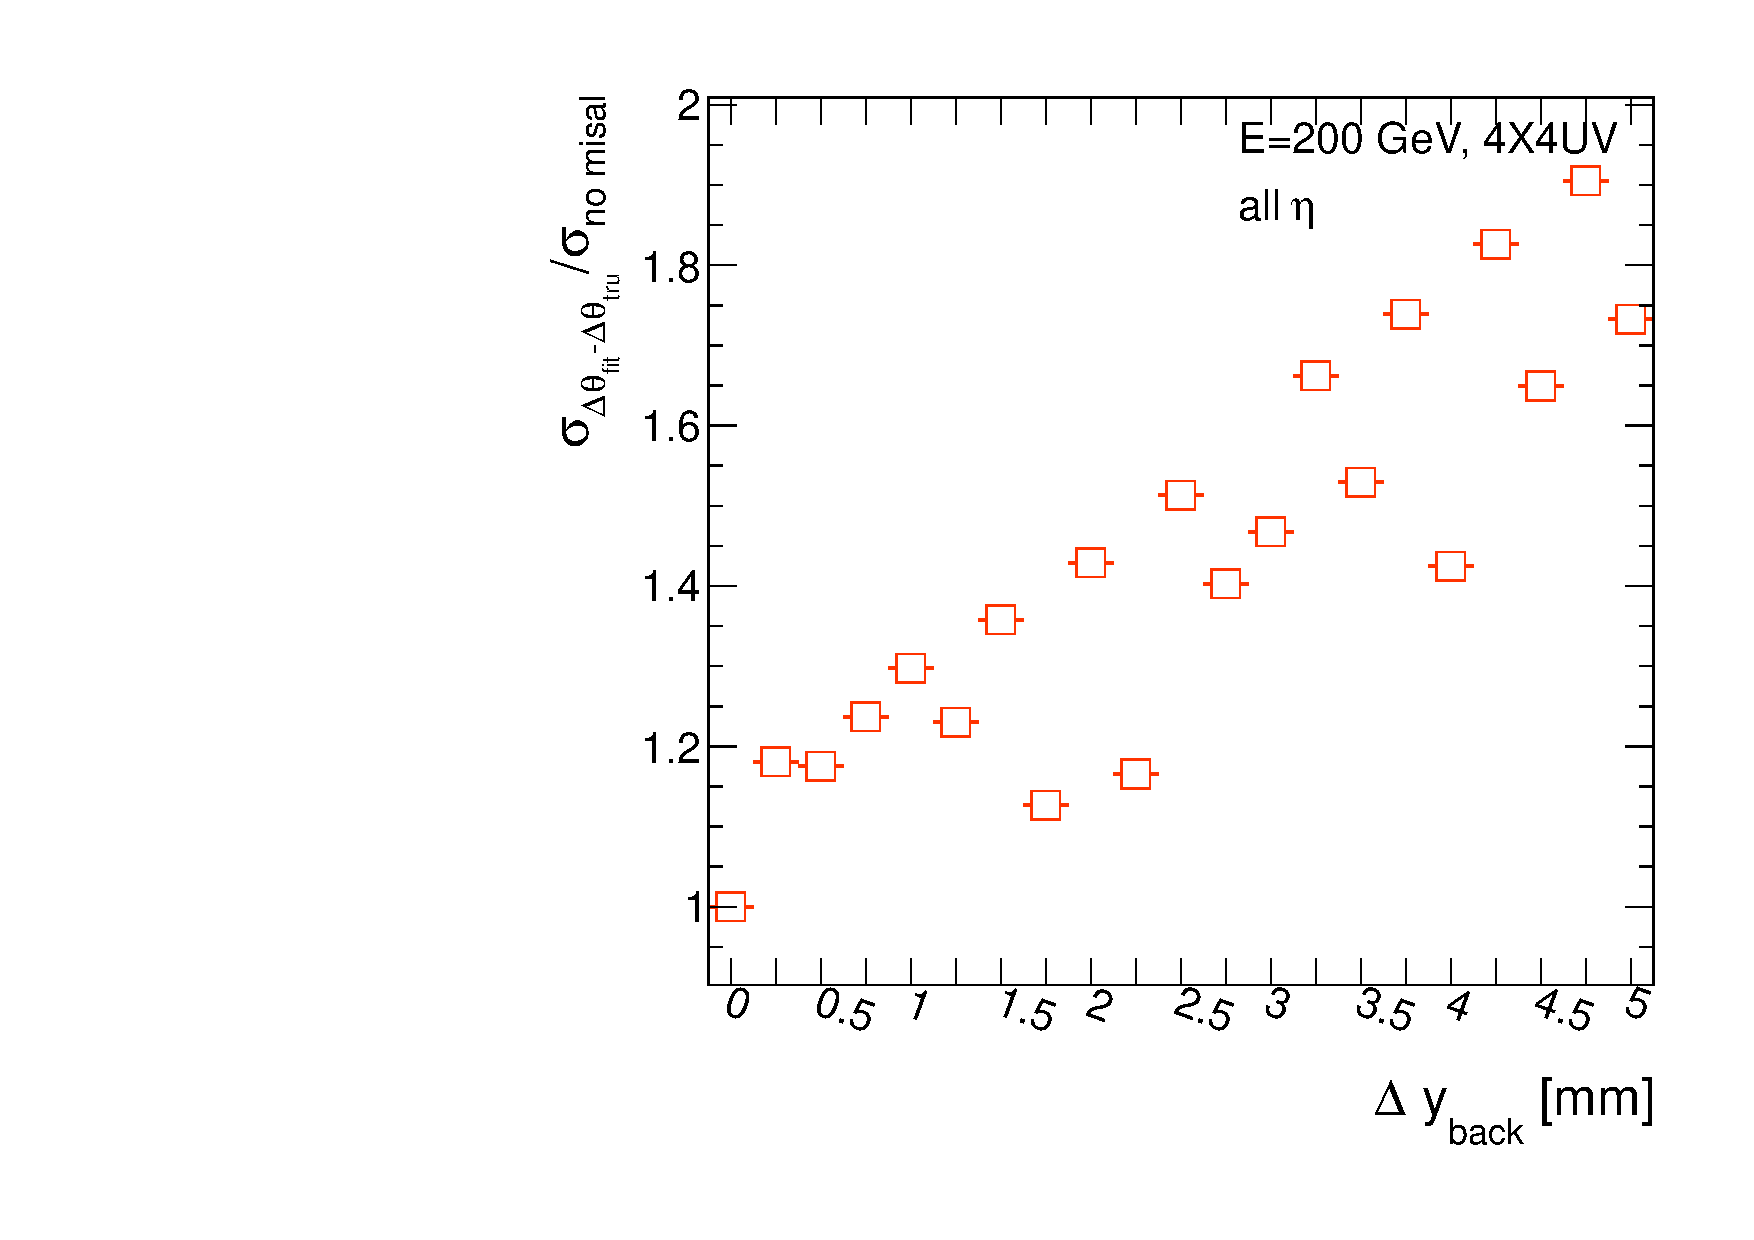
\includegraphics[width=0.32\textwidth]{algorithms-harvard/mmt_res_dtheta_misal_dyb_etaall_rel.pdf}
	}
	\subfloat[b][Top half shift in $r$]{
		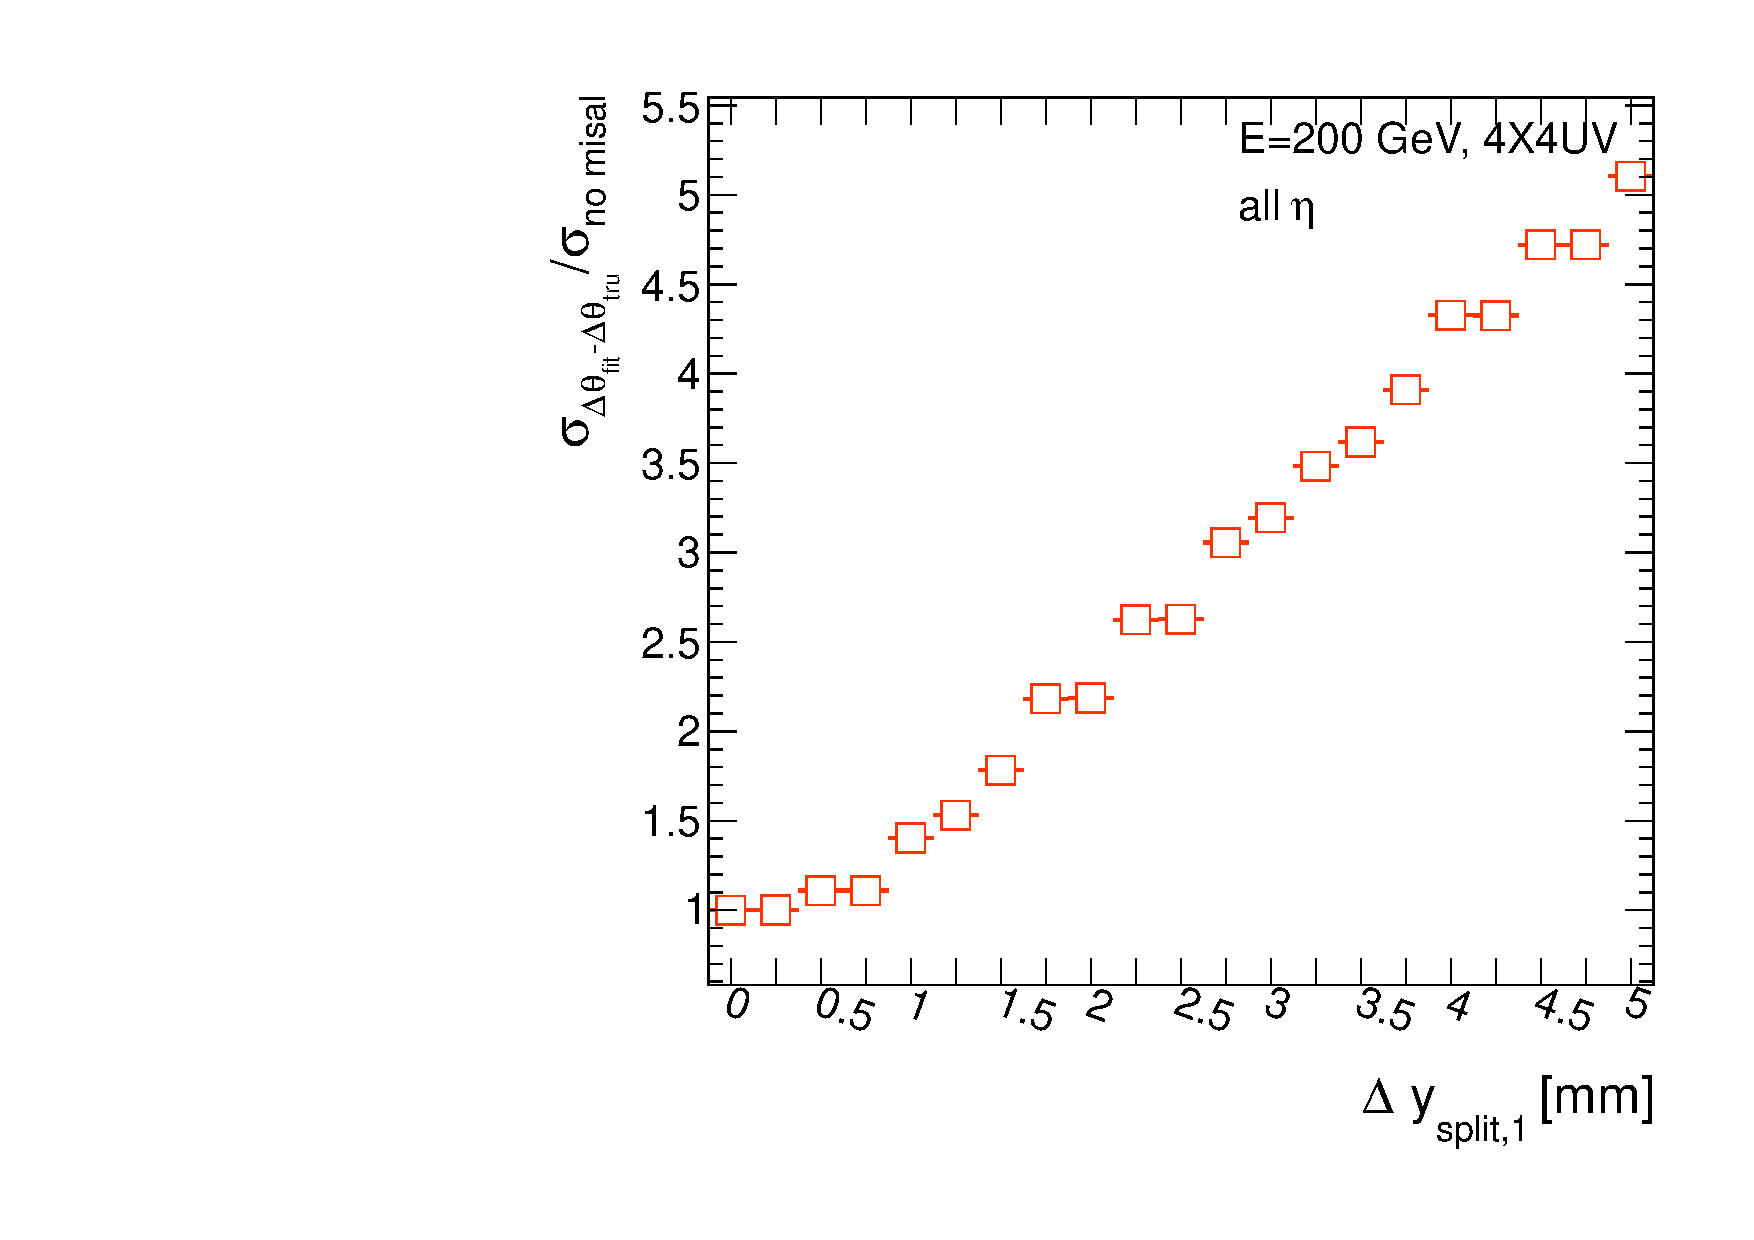
\includegraphics[width=0.32\textwidth]{algorithms-harvard/mmt_res_dtheta_misal_dyw1_etaall_rel.pdf}
	}
	\subfloat[c][$\phi$ rotation]{
		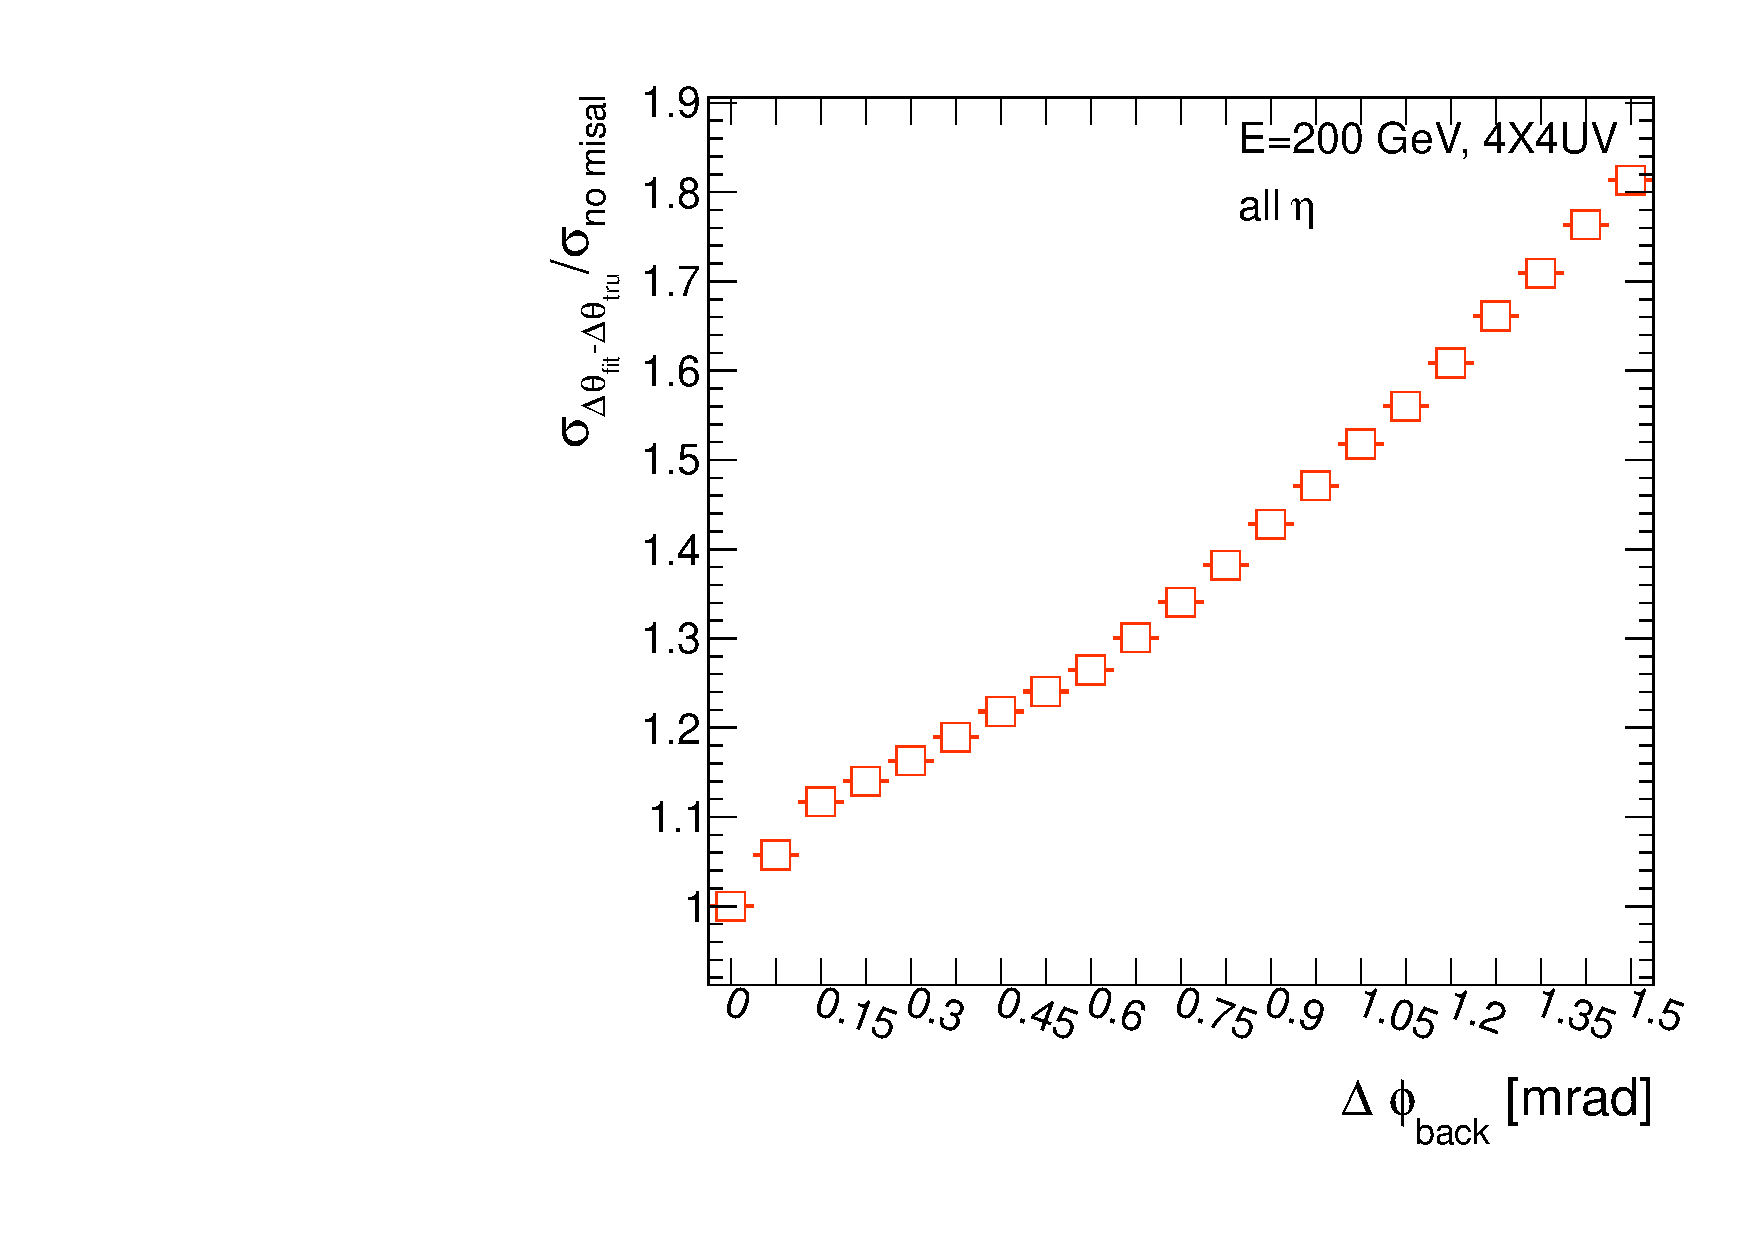
\includegraphics[width=0.32\textwidth]{algorithms-harvard/mmt_res_dtheta_misal_dpb_etaall_rel.pdf}
	}\\
	\subfloat[d][$\theta_{\rm tilt}$]{
		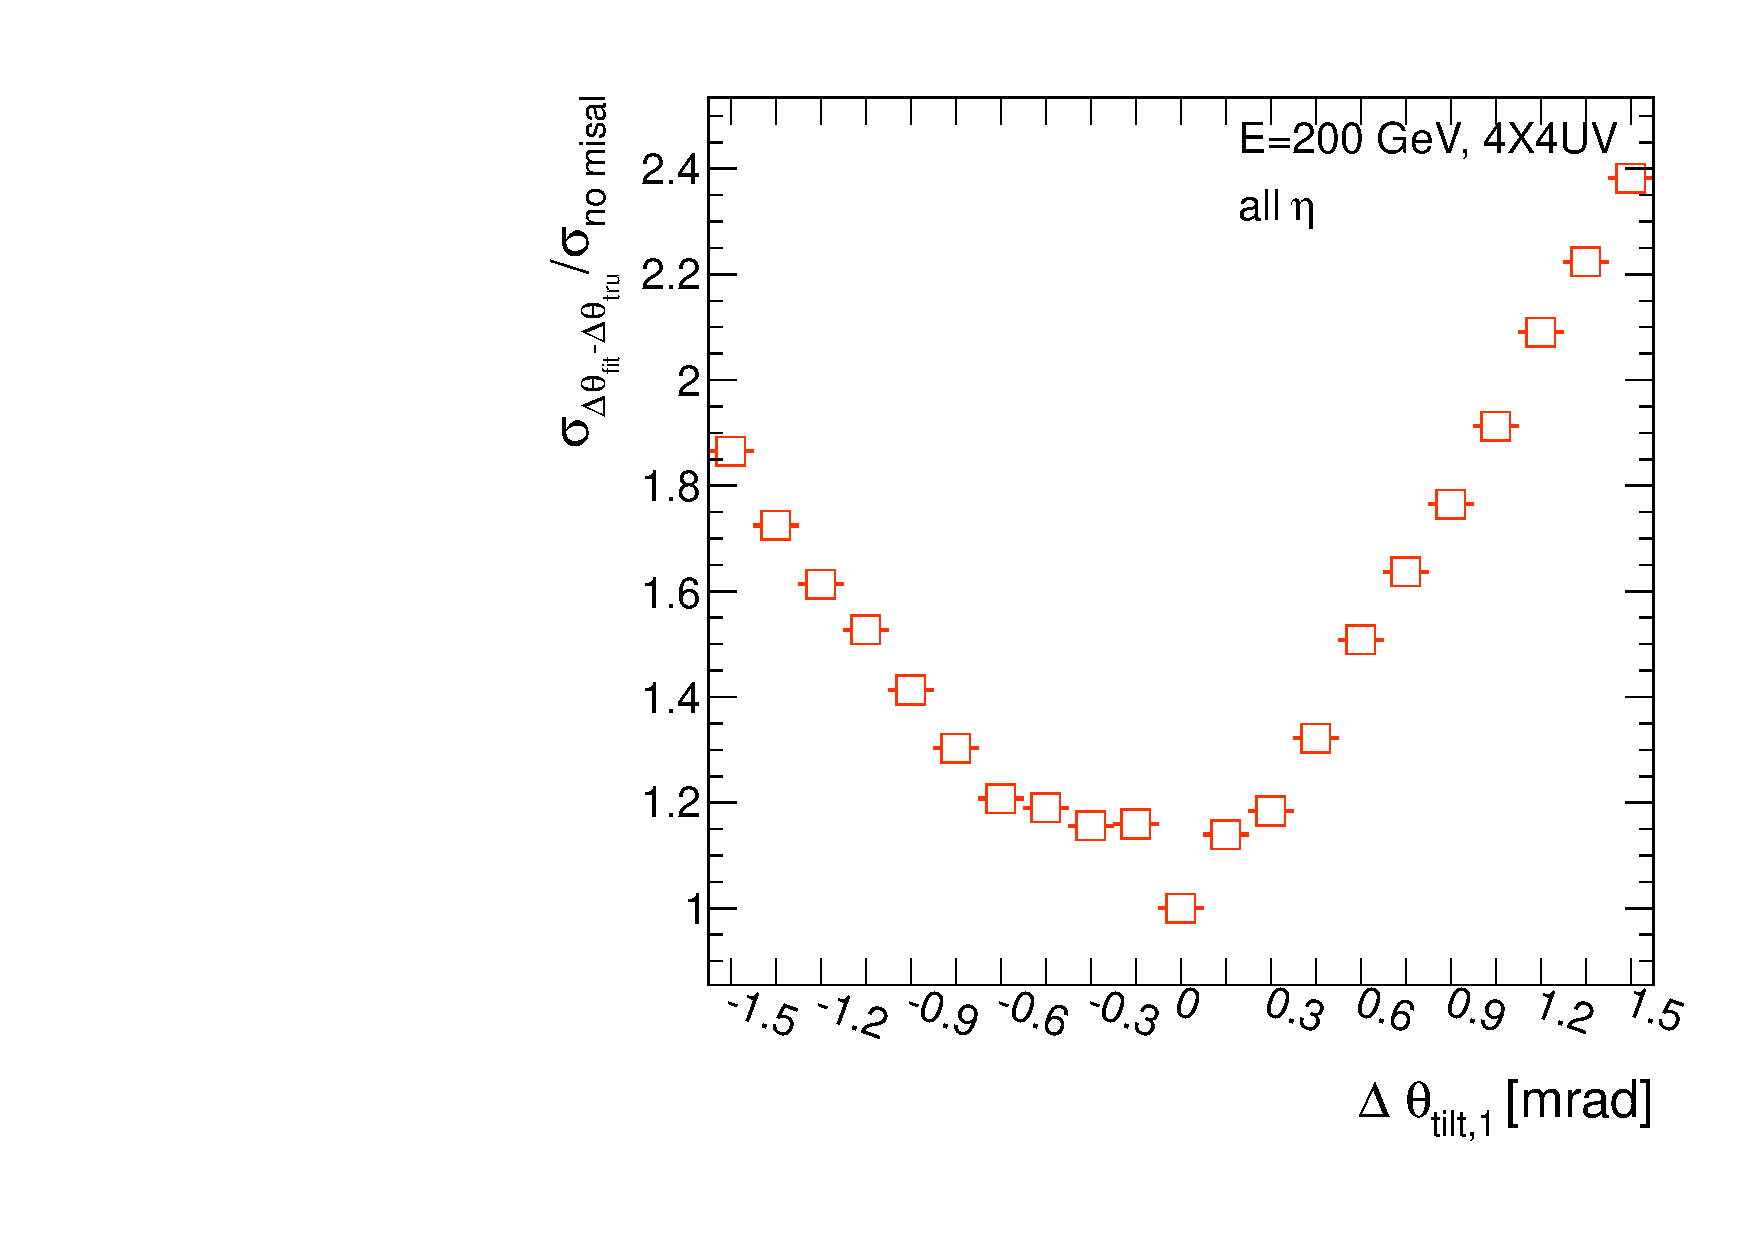
\includegraphics[width=0.32\textwidth]{algorithms-harvard/mmt_res_dtheta_misal_dt1_etaall_rel.pdf}
	}
	\subfloat[e][Shift in $z$]{
		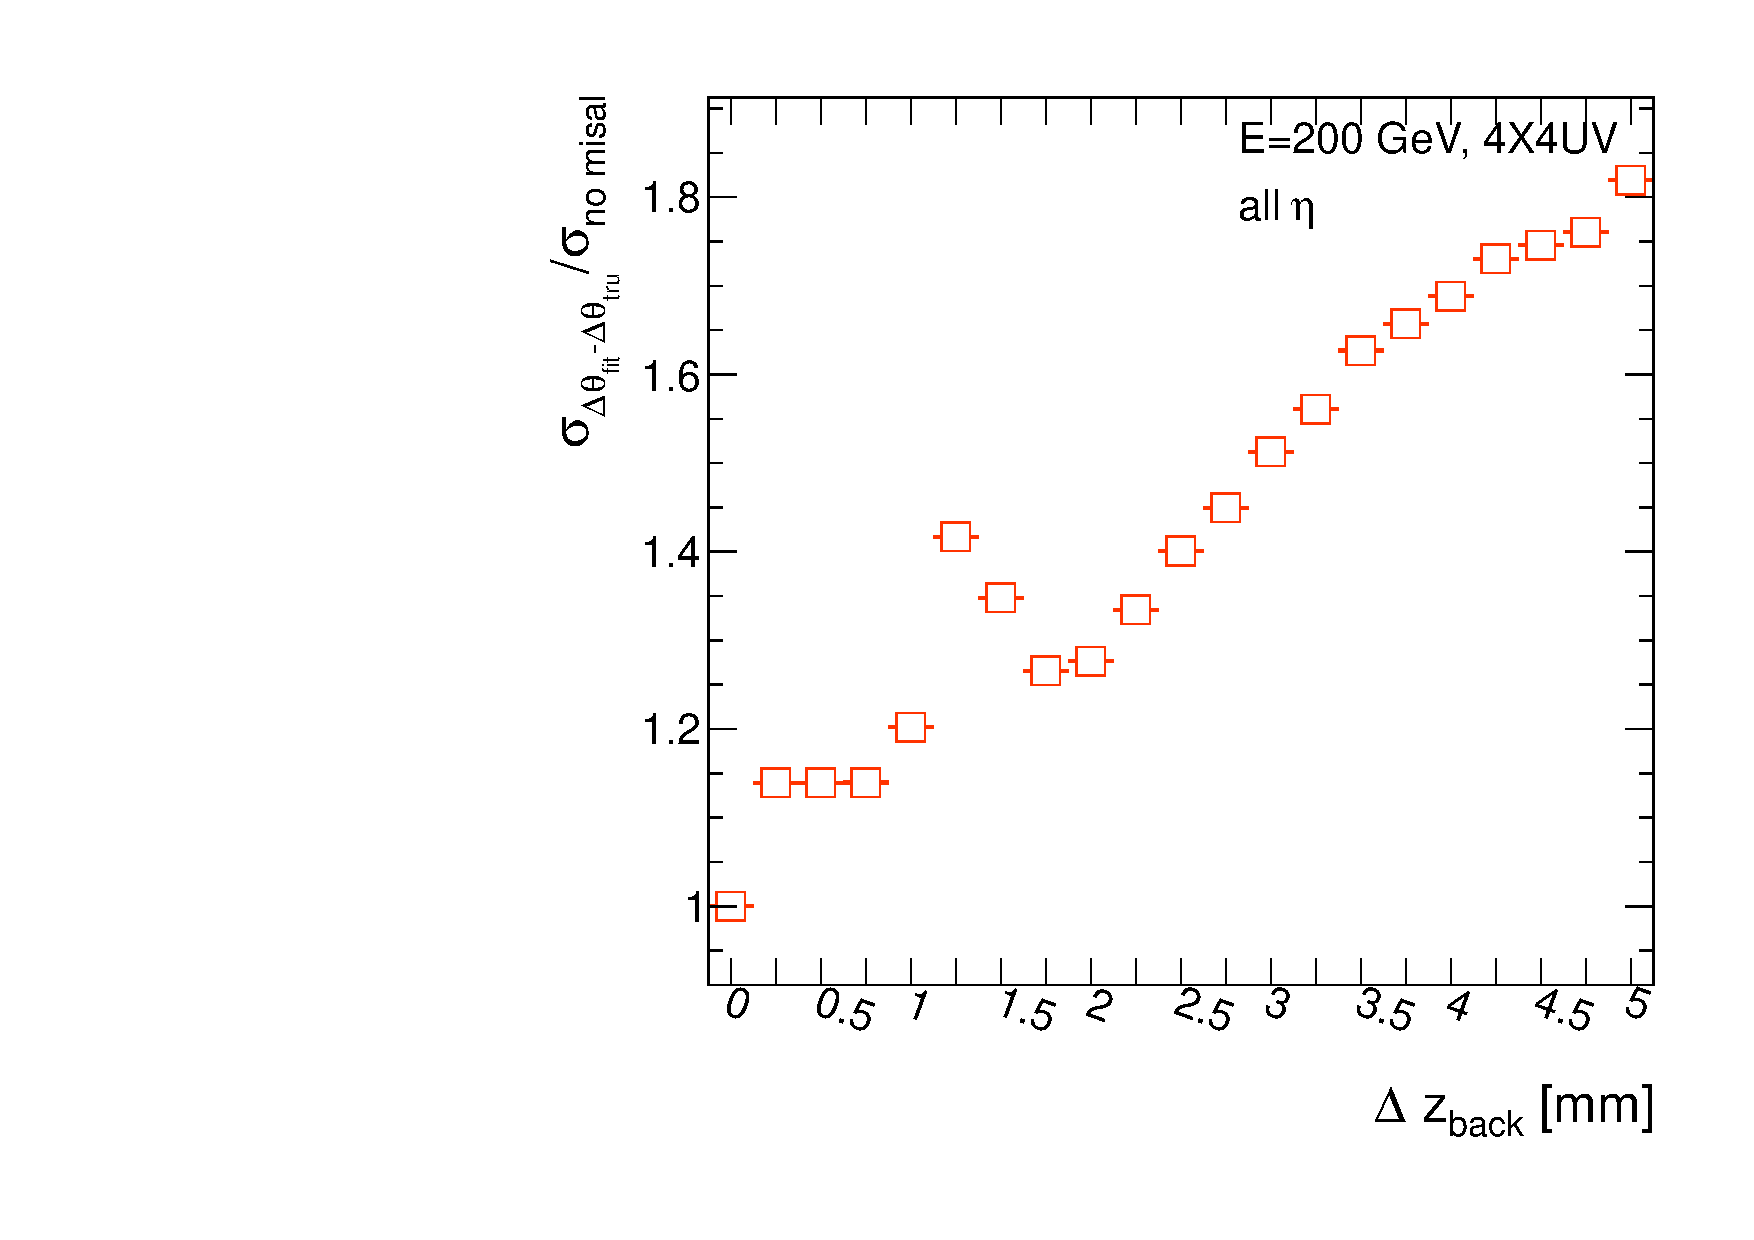
\includegraphics[width=0.32\textwidth]{algorithms-harvard/mmt_res_dtheta_misal_dzb_etaall_rel.pdf}
	}

	\caption{\label{fig:harvard_misal_effect}
	Relative change in $\Delta\theta^{\rm{fit}}$ resolution as a function of misalignment for different misalignment configurations.
	Figures (a)-(e) are laid out to match the corresponding misalignment as illustrated in Figure\,\ref{fig:harvard_misal_illustration}.
	}
\end{figure}

The degradation shows a certain periodicity related to strip width for displacements. This is clear for
Figures\,\ref{fig:harvard_misal_effect}\,(a) and~(b). The degradation is higher when only half of the
detector is radially shifted (b) because a double peak structure is formed, which increases more significantly
the peak width. Rotations (c and d) cause monotonic changes in performance. The degradation is more
significant when the tilt is away from the IP (positive axis) because more strips are forced to cover the same
solid angle, increasing the effective distance between the strip that should have been hit and the strip that
is actually hit. Figure\,\ref{fig:harvard_misal_effect}\,(e) shows at lower levels of misalignment a fixed level of degradation, again
caused by a discrete strip width. At around 1\,mm a two-peak structure appears in the distribution, which causes
an increase in the RMS. As the distribution gets further smeared the double peak structure disappears, yielding
a monotonically increasing degradation. Additional results can be found in Ref.~\cite{harvard-alg-misal}.

%These results are summarized in Table~\ref{tab:harv-misal}.
%\begin{table}
  %\centering
  %\begin{tabular}{|c|l|l|l|l|l|}%p{4.5cm}|}
    %\hline
    %Type          & $\Delta y_{back}$ & $\Delta y_{top}$ & $\Delta z_{back}$ & $\Delta\phi_{back}$ & $\Delta\theta_{tilt}$\\
    %\hline
   % Range studied &    0--5 mm        &   0--5 mm        &    0--5 mm        &    0--1.5 mrad      &    -1.5--+1.5 mrad   \\
    %\hline
    %25\%          &    0.75 mm        &     0.5 mm       &    1.25 mm        &       0.6 mrad      &    (-0.9)+0.45 mrad   \\
    %50\%          &     2.5 mm        &    1.25 mm       &     3.0 mm        &      1.05 mrad       &   (-1.05)+0.75 mrad   \\
    %\hline
   % Remarks       & \multicolumn{2}{|c|}{periodic in $w_{strip}$} & peak from geo. eff. & mono. inc. & +(-) is (away) twds. IP\\
    %\hline
  %\end{tabular}
  %\caption{\label{tab:harv-misal} Increase of resolution on $\Delta\theta$ error summary; levels of misalignment corresponding to \% increases in resolution are quoted.}
%\end{table}

It should be noted that corrections for all cases, except (c) have been developed. Based on these current
corrections, since only case (c) is relevant, a degradation
of up to 75\% on $\Delta\theta^{\rm{fit}}$ resolution (or from 1.7\,mrad to 3.0\,mrad in the 4-horizontal/4-stereo case) is
expected for 5\,mm misalignments.

\paragraph{Performance with the xxuv uvxx configuration}  \hfill \\
Recently, it has been decided to build sectors with the mirror-image placement (resulting
in a xxuv uvxx horizontal/stereo strip configuration). From the perspective of
the trigger, new simulations have not been produced yet. However, estimates of the improvement
in the $\Delta\theta^{\rm{fit}}$ resolution have been obtained\cite{harvard-alg-xxuvuvxx}.

The estimate has been performed using a
toy simulation of the trigger algorithm, which does not include any ionization or scattering effects.
This simulation only demonstrates resolution effects arising from the width of the strips. Based
on this simulation, an ideal geometrical $\Delta\theta^{\rm{fit}}$ resolution of 0.89\,mrad has been estimated for the
4-horizontal/4-stereo hit category in the standard geometry. This number can be used together
with the resolution obtained in the full simulation (and shown in Table\,\ref{tab:efficiencyHarvardIdeal})
to estimate the impact of different physics effects (ionization, multiple scattering...)
in the resolution. In particular, using $\sigma_{\rm athena}^2=\sigma_{\rm physics}^2+\sigma_{\rm geometry}^2$,
one can estimate $\sigma_{\rm physics}$. The toy simulation can then be used to calculate the new
$\sigma^{\rm new}_{\rm geometry}=0.79$ for the mirror-image geometry. This, combined with $\sigma_{\rm physics}$
provides the estimate of the quantity of interest $\sigma^{\rm new}_{\rm athena}$. Using this procedure,
one estimates that with the new geometry the ideal $\Delta\theta^{\rm{fit}}$ resolution for the 4-horizontal/4-stereo
hit category improves to 1.65\,mrad from 1.7\,mrad, or less than 5\%, in the case with backgrounds.
These studies are reported in more
detail in Ref.\,\cite{harvard-alg-xxuvuvxx} and need to be repeated using the ATLAS full simulation.

\subsubsubsection{Summary} 
An algorithm for the reconstruction of segments using trigger hits in the MM detector has been described. 
The algorithm has been tested using events passed through the ATLAS full simulation with a realistic detector geometry and 
description of the signal formation. The algorithm presented has a very high efficiency of close to 100\%, a 
position resolution
in $\theta$ and $\phi$ of $\approx 0.3$~mrad and $\approx 3$~mrad, respectively, and a $\Delta\theta$ resolution of 
$\approx 1.7$~mrad. The algorithm has also been tested in conditions including incoherent background at realistic rates, showing
very comparable performance, except on the $\phi$ resolution, which degrades to $\approx 5$~mrad. 
To achieve high efficiency, relatively loose requirements on the number of hits (2 horizontal strips and one stereo
strip) need to be imposed. Tighter requirements, which might prove necessary to reject backgrounds, can be applied. A requirement
of 3 horizontal and 3 stereo strip hits yields an efficiency of about 92\%. 

The algorithm has been implemented in a Virtex XC7VX485T FPGA and its latency has been estimated with this
set-up at 56\,ns for the current implementation, using a 320~MHz clock. Memory resources have also been
estimated using this set up and fall well within the capabilities of this FPGA with a 30\% margin. This simulation
does not include some additional functionality, such as misalignment corrections or ancillary functions, so the
possibility of using a pin-compatible FPGA with higher resources is currently being investigated. 

Misalignment conditions have been simulated using truth hit information from the ATLAS full simulation. Misalignments of
up to 5\,mm have been considered. No significant changes in algorithmic efficiency, $\phi$ or $\theta$ resolution have 
been observed. The reconstruction of $\Delta\theta$ is affected by these misalignments. In particular, a significant
degradation of the resolution has been observed. Corrections requiring low resources in the FPGA have been 
described for four out of the five types of misalignments surveyed. For the fifth type, corrections can be designed, 
but they would increase the latency of the algorithm and their impact on the overall resources needs to be studied. 
Estimates have been provided for the degradation in the $\Delta\theta$ resolution for this case of at most 75\%, resulting
in a resolution of 3.0\,mrad for sectors with local misalignments of 5\,mm. 

\FloatBarrier

%-------------------------------------------------------------------------------
\subsubsection{MM Look-Up-Table Algorithm}
\label{sec:algorithms-saclay}
%Description, implementation, alignment corrections, performance and latencyFigure\,\ref
%%%%%%%%% Sample inclusion of a figure
 % \begin{figure}[h]
 % \begin{center}
 % \includegraphics[width=0.8\textwidth]{algorithms-saclay/Plot1}
 % \caption{Caption of plot 1}
 % \label{fig:Monitoring}
 % \end{center}
 % \end{figure~\ref{fig:}}
%%%%%%%%%%%%%%%%%%%%%%
\FloatBarrier
 \subsubsubsection{Principle of the algorithm}
%%%%%%%%%%%%%%%%%%%%%%
The eight MM layers that form a large sector are numbered from 1 to 8 (1, 2, 5 and 6 being the $X$ layers, 3 and 7 the $U$ layers, and 4 and 8 the $V$ layers) and grouped in pairs: $(1, 5), (2, 6), (3, 7), (4, 8), (1, 6)$ and $(2, 5)$, so six pairs in total. When a muon passes through the detector, hits are created on each of the layers. For each considered pair, the first strips that triggered  for both layers of the pair are used to calculate the corresponding slope with the formula:
$${\rm slope_{pair}}=\frac{y_{\rm layer2}- y_{\rm layer1}}{z_{\rm layer2}- z_{\rm layer1}}$$
where $y_{\rm layer1,2}$ and $z_{\rm layer1,2}$ are the strip positions in the $(y,z)$ plane. Figure\,\ref{fig:SaclayTriggerPrinciple} illustrates the pair selection and the angle calculation with respect to the interaction point (IP). The distance between layer pairs (1,\,5), (2,\,6), (3,\,7) and (4,\,8) is of 126\,mm, 137\,mm for pair (1, 6) and 115\,mm for pair (2, 5) respectively as shown in Figure\,\ref{fig:SaclayAlgorithmPair}.

%%%%%%%%%%%%%%%%%%%%%%
 \begin{figure}[htb!]
  \begin{center}
  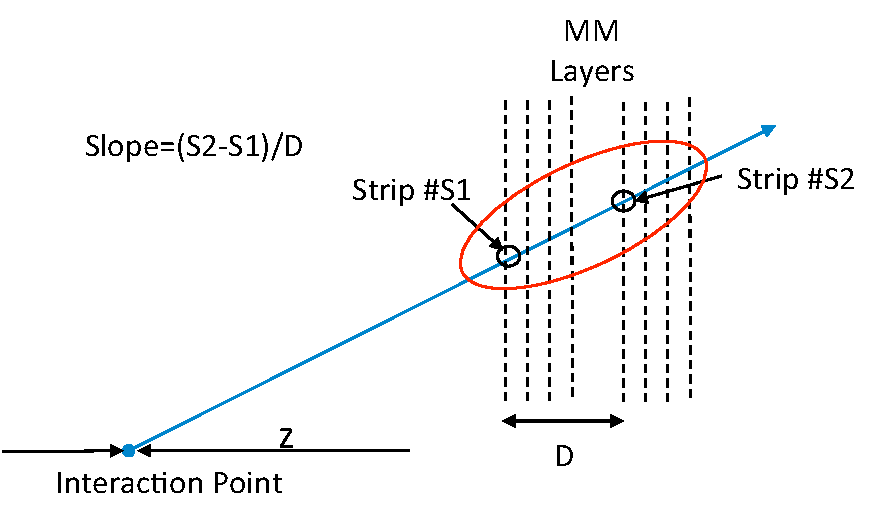
\includegraphics[width=0.5\textwidth]{algorithms-saclay/SaclayTriggerPrinciple.pdf}
  \caption{Illustration of pair selection and angle calculation with respect to the interaction point.}
  \label{fig:SaclayTriggerPrinciple}
  \end{center}
  \end{figure}
%%%%%%%%%%%%%%%%%%%%%%
 \begin{figure}[htb!]
  \begin{center}
  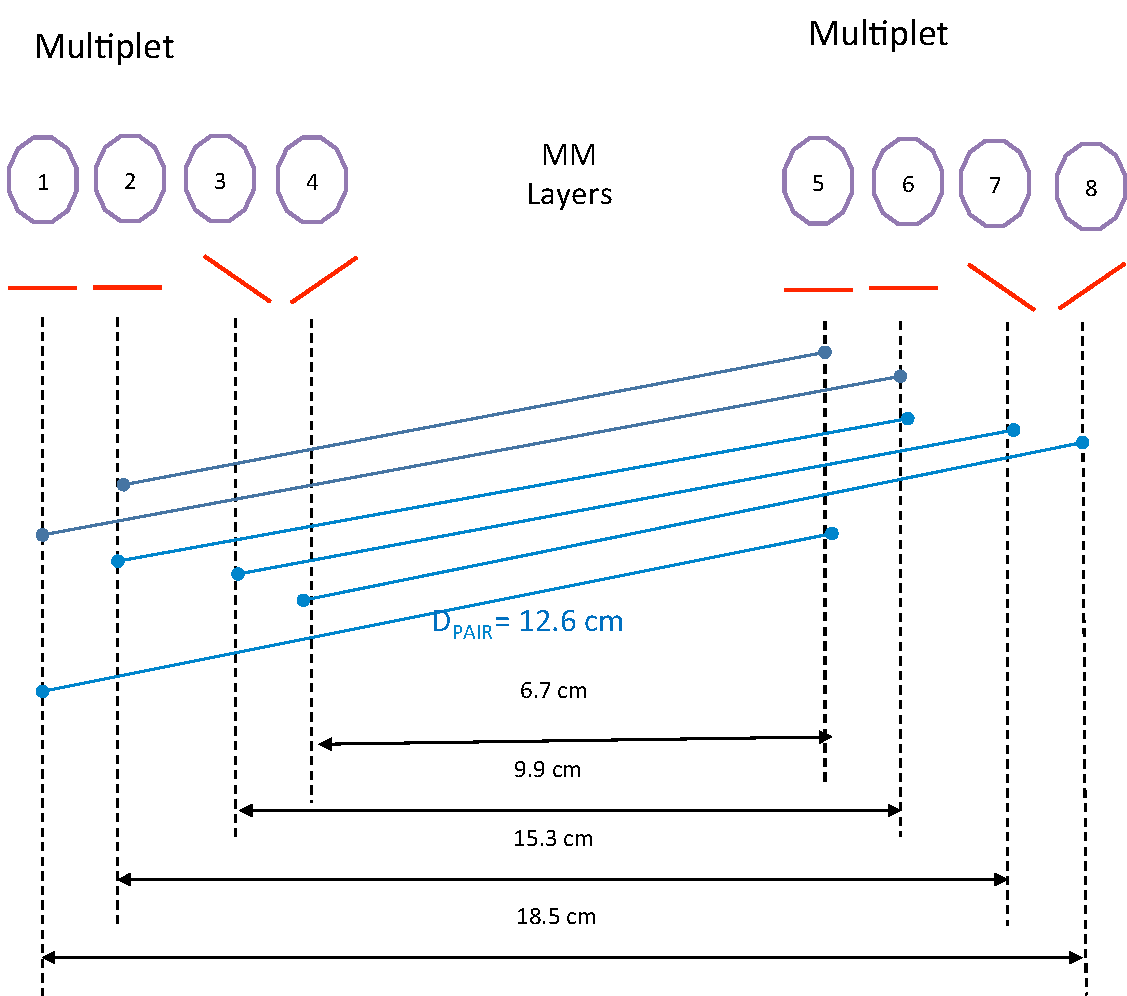
\includegraphics[width=0.55\textwidth]{algorithms-saclay/SaclayAlgorithmPair.pdf}
  
\includegraphics[width=0.7\textwidth]{algorithms-saclay/SaclaySlopeComaprison.pdf}
  \caption{Representation of pairs formed by the algorithm (top) and comparison between the slopes (bottom).}
  \label{fig:SaclayAlgorithmPair}
  \end{center}
  \end{figure}
%%%%%%%%%%%%%%%%%%%%%%
The so calculated slopes are then compared to each other as  shown in Figure\,\ref{fig:SaclayAlgorithmPair}. If a certain number of them (above some threshold value defined in the selection logic) are equal within a given precision, they are considered as forming a unique track corresponding to one muon and retained for further processes. All these calculations are done locally; the condition of a pointing track (i.e.\ coming from the interaction point) is then added in order to determine the Regions of Interest (RoI).

In this study, the detector is segmented in several panel regions which correspond originally to the segmentation in four chambers. With the present design, with only two chambers, the panels correspond to the logical segmentations (for instance, two or more panel or regions per chamber).
Figure\,\ref{fig:SaclayElectronicImplementation} shows the electronic implementation of the trigger for two bunch crossings (BC) for one panel region.
In order to allow for noise, multiple hits and multiple muons in a given panel region, up to 8 hits per layer and per BC can be considered by the algorithm. Hence, for each layer pair, a maximum of $8\times 8=64$ slopes is calculated. For 2~BC there are 4 sets of 6 layer pairs with 64 slopes calculation for each pair.
The algorithm described above intervenes at the ``SLOPE SELECT'' step in Figure\,\ref{fig:SaclayElectronicImplementation}, pre-selecting the track candidate for further processing. Performance and latency are also given in Figure\,\ref{fig:SaclayElectronicImplementation} assuming 320\,MHz tic frequency.
%%%%%%%%%%%%%%%%%%%%%%%
 \begin{figure}[htb!]
  \begin{center}
  
\includegraphics[width=0.98\textwidth]{algorithms-saclay/SaclayElectronicImplementation.pdf}
  \caption{Electronic implementation for one panel region.}
  \label{fig:SaclayElectronicImplementation}
  \end{center}
  \end{figure}
%%%%%%%%%%%%%%%%%%%%%%
%%%%%%%%%%%%%%%%%%%%%%
 \subsubsubsection{Algorithm Implementation}
%%%%%%%%%%%%%%%%%%%%%%
The algorithm performance is essential to respect the requirements on the trigger response time: a decision has to be made in less than 100\,nanoseconds. So to limit the number of calculations, the solution of a Look Up Table (LUT) has been retained. Its operating principle is as follows. \\
For each layer pair, a panel region  corresponds to a given range aperture angles from the IP as illustrated in Figure\,\ref{fig:SaclayAngleAperture}. These  aperture angles are delimited by the borders between the adjacent panel regions.
Based on simple geometrical considerations, it is possible to store all the possible values of the slopes (difference between strip numbers of the two layers) that a pointing track can have in a given panel region with a certain granularity in a 32 bits register.
Then for each layer pair, a Look Up Table is used to check  whether each of the 64 slopes is within the range of allowed values for this panel as presented in Figure\,\ref{fig:SaclayLUTprinciple}. As an output, each time a matching is found,  a bit  is filled in a 32-bit register which corresponds to the slope value.  Bit 0 is filled in case of no-match. For each layer pair, there are four such registers  corresponding to the four possible BC combinations. \\
In the following step of ``Slope Select Logic'' in Figure\,\ref{fig:SaclayElectronicImplementation}, the registers corresponding to the six layer pairs are compared. If there are minimum number of compatible values within a given precision (for example within two slope bits),  the combination is considered as valid and is kept for further process.  The track candidate slope is then determined by the average slope of the accepted segments. Track constraint to the IP could be implemented in the future.

In order to account for the larger distance from the IP of the second multilayer, projective panel region are defined which are slightly different from the physical  segmentation. The principle is depicted on Figure\,\ref{fig:SaclayProjectivePR}.
%%%%%%%%%%%%%%%%%%%%%%%
 \begin{figure}[htb!]
  \begin{center}
  
\includegraphics[width=0.65\textwidth]{algorithms-saclay/SaclayAngleAperture.pdf}
  \caption{Angle aperture for different panel regions.}
  \label{fig:SaclayAngleAperture}
  \end{center}
  \end{figure}
%%%%%%%%%%%%%%%%%%%%%%%%
%%%%%%%%%%%%%%%%%%%%%%%
 \begin{figure}[htb!]
  \begin{center}
  
\includegraphics[width=0.65\textwidth]{algorithms-saclay/SaclayLUTprinciple.pdf}
  \caption{Operating principle of the LUT.}
  \label{fig:SaclayLUTprinciple}
  \end{center}
  \end{figure}
%%%%%%%%%%%%%%%%%%%%%%%%
%%%%%%%%%%%%%%%%%%%%%%%
 \begin{figure}[htb!]
  \begin{center}
  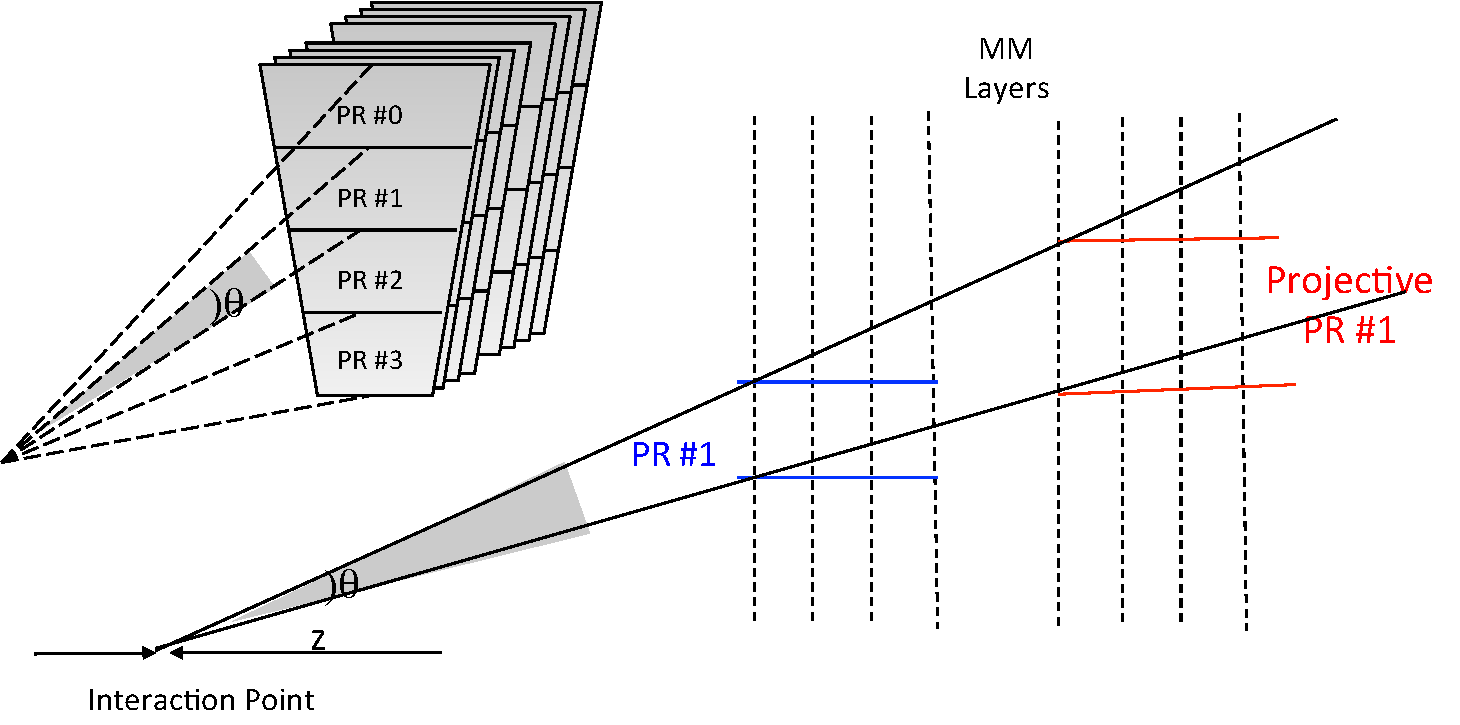
\includegraphics[width=0.7\textwidth]{algorithms-saclay/SaclayProjectivePR.pdf}
  \caption{Implementation of projective panel regions.}
  \label{fig:SaclayProjectivePR}
  \end{center}
  \end{figure}
%%%%%%%%%%%%%%%%%%%%%%%%
%\textbf{Construction of the Look Up Table} : The first step to construct the LUT is to determine the angles delineating the four panel regions. To do so, the simulation has been used to identify the $y$-coordinates where hits are missing, i.e. the boundaries between the panel regions. Their analysis allows to determine their corresponding angles from the IP by the formula $\theta_{d}=\frac{y_{\rm layer0}}{z_{\rm layer0}}$ and the corresponding slopes of these angle given by their tangents $\tan(\theta_{d})$. The aperture angle $\theta_{d}$ should be slightly different for each layer because of the different distances from the IP; but it has been observed that these differences are too small (the layers are distant of a few centimeters from each other and about seven meters from the IP) to change the results so they are considered as negligible.
%
%The Table~\ref{tab:NsLUT}The aperture angles obtained thanks to these informations for each panel regions and the numbers of strips $N_{s}$ corresponding to these aperture angles are grouped in the Table~\ref{tab:NsLUT}. The formula used is:
%$$N_{s}=\frac{D_{2} }{ l_{p}}=D_{pair}\times \frac{\tan(\theta_{dfi}) - \tan(\theta_{dsi})}{l_{p} }$$
%where $i$ vary from 0 to 3 for the angles of the dead zones, and where $D_{2}$ is depicted in Figure\,\ref{fig:SaclayAngleAperture}. $l_{p}$ is
%the pitch between the beginning of strip and the beginning of the following one, and $D_{pair}$ is the distance between the two layers of the pair.

\textbf{Construction of the Look Up Table} : the aperture angles are obtained from the simulation as shown in Figure\,\ref{fig:SaclayAngleAperture}. The Table~\ref{tab:NsLUT} gives these aperture angles as well as the expected maximum value of difference of slopes expressed in term of number of strips  ($N_{s}$ ).
$N_{s}$ depends of the distance between the two layers of the pair; the numbers given in the Table\,\ref{tab:NsLUT} are for the pairs of 126~mm distance. These numbers are slightly smaller for the pair of 115\,mm and slightly higher for the pair of 137\,mm.

%%%%%%%%%%%%%%%%%
\begin{table}[h!tbp]
\centering
\begin{tabular}{ c  c  c }
\toprule
Panel region & Aperture angle ($^{\circ}$) & Number of strips ($N_{s}$) \\
\midrule
0 & 4.73 & 31\\
1 & 5.93 & 36\\
2 & 6.45 & 36\\
3 & 6.86 & 36\\
\bottomrule
\end{tabular}
\caption{Number of strips for the LUT in each panel region}
\label{tab:NsLUT}
\end{table}
%%%%%%%%%%%%%%%%%%
%
%So for each panel region, $N_{s}$ slopes corresponding to the possible strips given the aperture angle are calculated and stored into the LUT. Ideally, when a muon passes through the detector and the slopes are determined for each pair, these slopes have to be exactly equal to one of the
%slope of the LUT for the track being considered as valid. But it appears that a number of pre-calculated slopes superior to 32 in a given panel region of the LUT is too high for the electronic logic. So the choice has been made, instead of calculating $N_{s}$ slopes per panel region for the LUT, to divide the aperture angle in 31 bins and one bin equal to zero and reserved in case of non-matching. This way, it is sufficient that the slope of the pair included in one bin of the
%LUT instead of being exactly equal to one of the pre-calculated slope. When the six slopes are considered as valid by the LUT, the track candidate slope is then determined by the average slope of the six segments.
%
%%%%%%%%%%%%%%%%%%%%%%
 \subsubsubsection{Algorithm Performance}
%%%%%%%%%%%%%%%%%%%%%%
The algorithm is tested using simulated sample of dimuon events.The simulated samples consist of $385\,000$ dimuon events with one muon per end-cap with the old MM layout containing four panel regions. The muons are originating from the IP and are uniformly distributed both in transverse momentum ($4~< p_{T}~<100$~GeV) and in the $\phi$ coordinate. In the $\eta$ coordinate, they are flat in the range $1<|\eta|<3.2$. This study is performed  without any background simulation.

%%%%%%%%%%%%%
 \textbf{Slope comparison} : assuming the ideal case of events with eight hits (with one hit per layer), the difference between the six slopes values is shown in Figure\,\ref{fig:SaclayLUToptimisation}(a). The differences are spiked in zero, but the RMS of 0.005 shows that the hit strip in the multilayers can only be known with a precision of $\pm 2$ strips. The tail goes up to $\pm 10$  strips.
This is due do the known ionization problem : the earlier strip hit within a VMM, is not always the closest to the real track. So in the LUT, it often happens that more than one bin match the track candidate. The right plot in Figure\,\ref{fig:SaclayLUToptimisation}(b) shows the number of bins hit in
the LUT (the bin 2, for example, means that the six slopes of the track candidate span two different bins in the LUT). This problem
complicates the electronic implementation but fortunately the bottom plot in Figure\,\ref{fig:SaclayLUToptimisation}(c) shows that most of the time, if different bins are hit in the LUT, they are directly adjacent. This property makes the electronics scan of hit bins in the LUT feasible.
%%%%%%%%%%%%%
%%%%%%%%%%%%%%%%%%%%%%%
 \begin{figure}[htb!]
  \begin{center}
  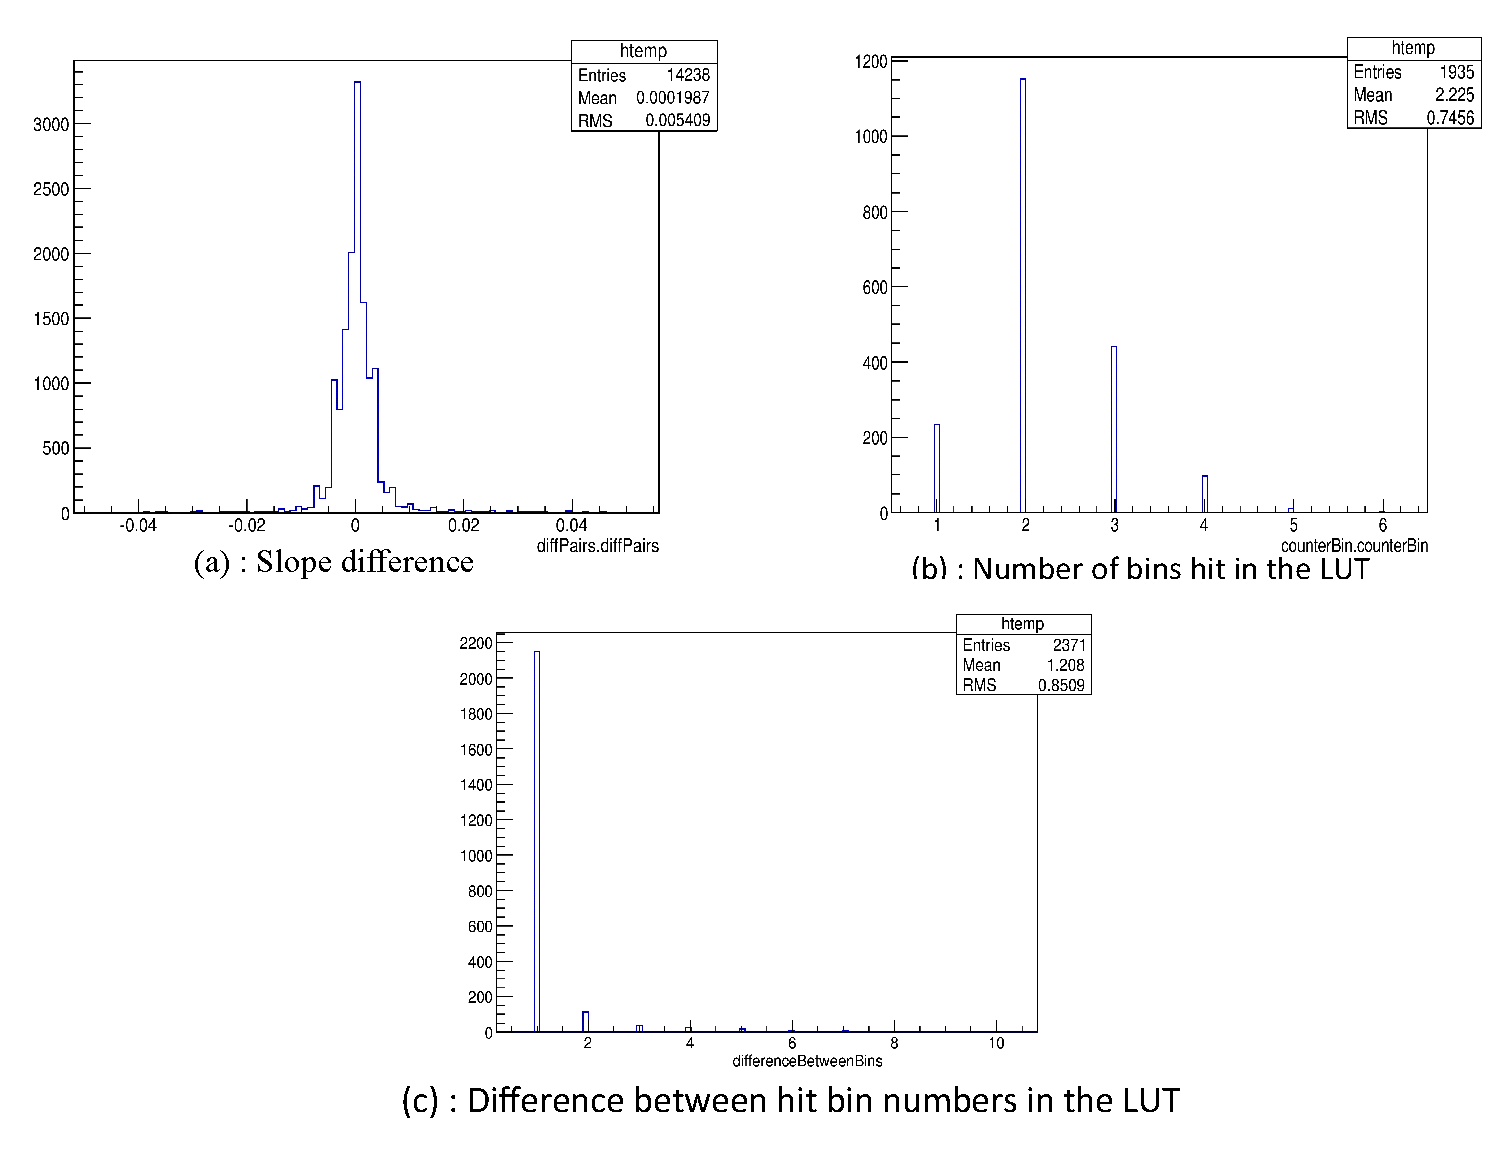
\includegraphics[width=0.99\textwidth]{algorithms-saclay/SaclayLUToptimisation.pdf}
  \caption{(a) : Difference of slope values. (b) Number of bins hit in the LUT. (c) Difference between hit bins in the LUT. }
  \label{fig:SaclayLUToptimisation}
  \end{center}
  \end{figure}
%%%%%%%%%%%%%%%%%%%%%%%%

%%%%%%%%%%%%%%
 \textbf{Intrinsic Efficiency} : The efficiency of the algorithm is defined as the ratio between the number of tracks which passed the algorithm requirement
and the total number of simulated tracks. The efficiency is calculated for the ideal case of events with eight hits (with one hit per layer).
 Figure\,\ref{fig:SaclayEfficiencyVsEtaPt}  shows the intrinsic efficiency as a function of $\eta$ and $p_{T}$
The holes observed in the efficiency distribution versus $\eta$ are explained by the gaps between the different panel regions located at $\eta \simeq 1.43, \eta \simeq 1.68$ and $\eta \simeq 2.05$. Indeed some track candidates overlap two panel regions and so cannot be taken into account by the LUT (which is defined per panel region). The global efficiency of the algorithm is 99.6\% for projective panel regions and 99.2\% otherwise. This inefficiency  cannot be fully recovered since the electronic implementation is not fully projective.
%%%%%%%%%%%%%%
  \begin{figure}[htb!]
  \centering
  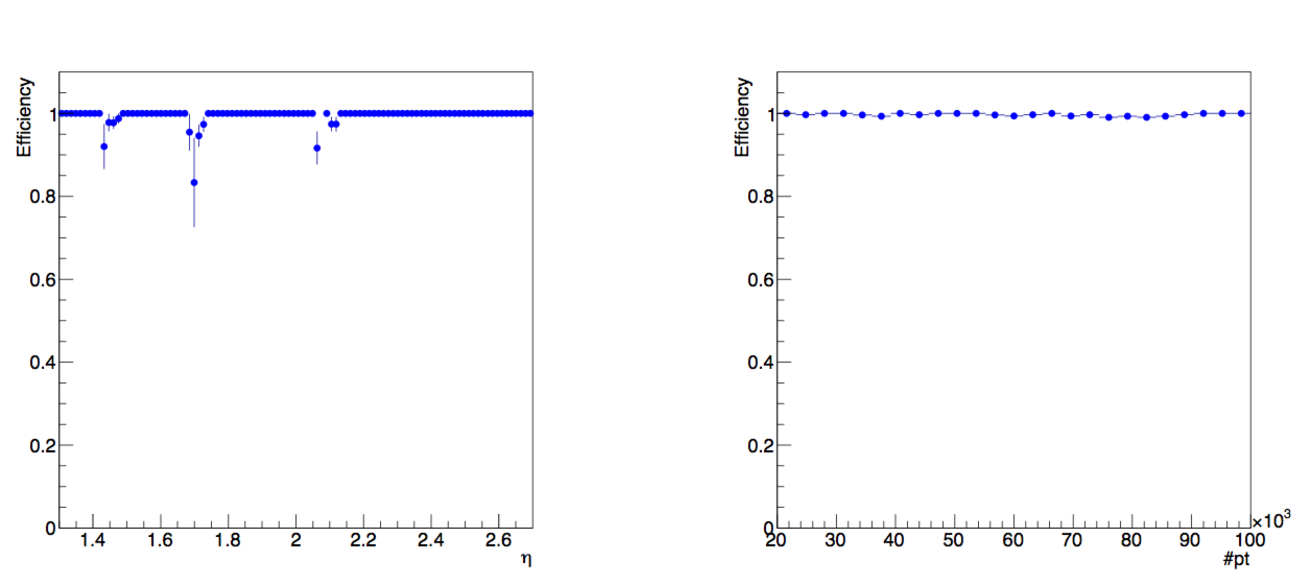
\includegraphics[width=0.95\textwidth]{algorithms-saclay/SaclayEfficiencyVsEtaPt.pdf}
  \caption{Distribution of efficiency versus $\eta$ (left) and $p_{T}$ (right) in the ideal case of eight hits (one hit per layer).}
  \label{fig:SaclayEfficiencyVsEtaPt}
  \end{figure}
%%%%%%%%%%%%%%%%%%%%%%%%

\textbf{Efficiency for six hits} : the efficiencies for  different pair requirements are shown in Figure\,\ref{fig:SaclayEfficiencyForDifferentPairRequirement}: the pairs $U$ and $V$ with four, three or two pairs $X$, and the pair $U$ or $V$ with four, three, two or one pair $X$. It is mandatory to have at least one pair $X$ to have the $\eta$ coordinate with enough precision and one of the two pairs $U$ and $V$ to determine the $\phi$ coordinate. These efficiencies are calculated in the case of only six hits (it may happens that hits are missing because the track passes through a gap between two panel regions).
For comparison, the efficiency of the Harvard algorithm with a requirement of only two layers $X$ and the layers $U$ and $V$ is of 99\%. The Saclay algorithm loses more information when hits are missing (because when one hit is missing in one layer, the pair cannot be built, so the informations of two hits is lost (and of four hits if the hit is missing on a $X$ layer), which explains this efficiency difference. However, the method of pairs should be more robust and precise for background filtering and rejection.
%%%%%%%%%%%%%%
  \begin{figure}[htb!]
  \centering
  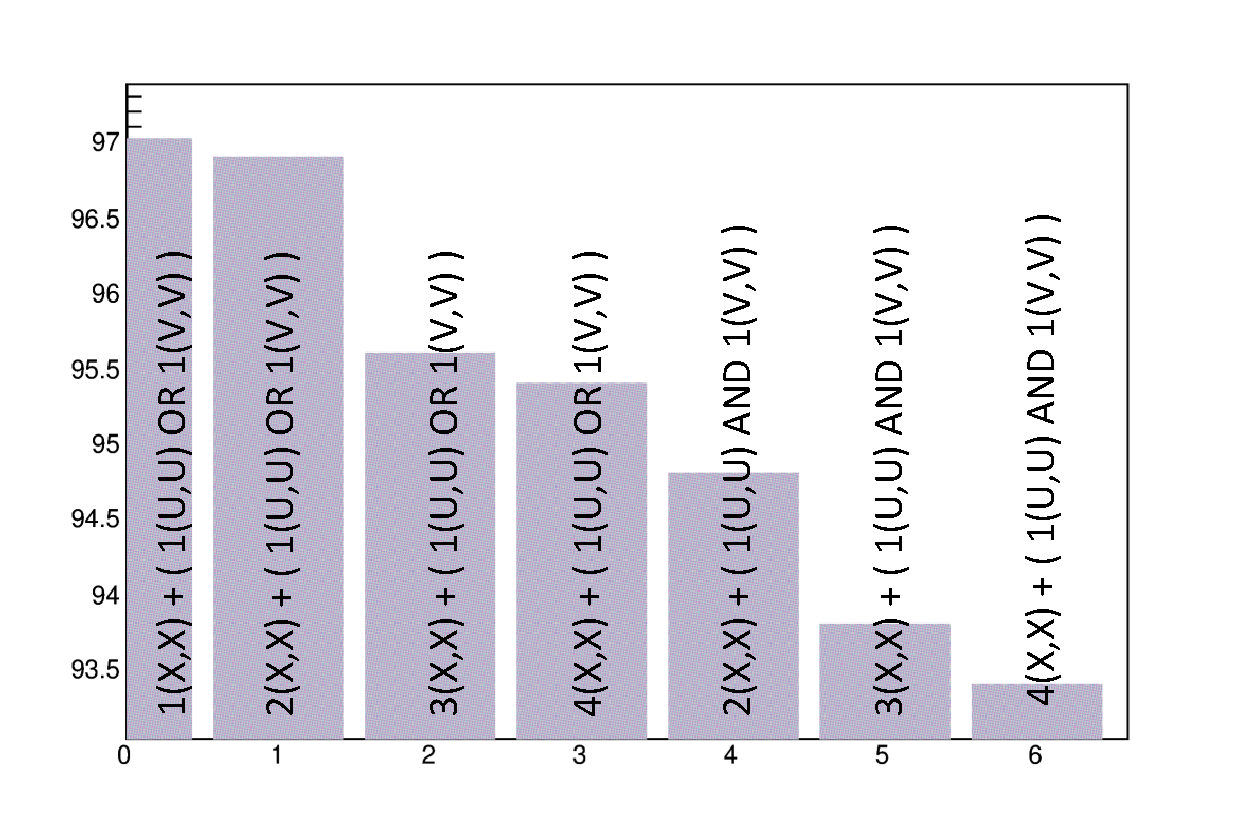
\includegraphics[width=0.55\textwidth]{algorithms-saclay/SaclayEfficiencyForDifferentPairRequirement.pdf}
  \caption{Efficiencies for different pair requirements in the case of six hits.}
  \label{fig:SaclayEfficiencyForDifferentPairRequirement}
  \end{figure}

 %%%%%%%%%%%%%
 \textbf{Resolution} : the resolution at the muon spectrometer entrance is calculated as the difference between the angle $\theta_{rec}$ as reconstructed by the algorithm and $\theta_{truth}$ as simulated at the muon spectrometer entrance. The RMS of this distribution shown in Figure\,\ref{fig:SaclayResolution} gives a resolution of 1.7\,mrad.
 %%%%%%%%%%%%%
%%%%%%%%%%%%%%
  \begin{figure}[htb!]
  \centering
  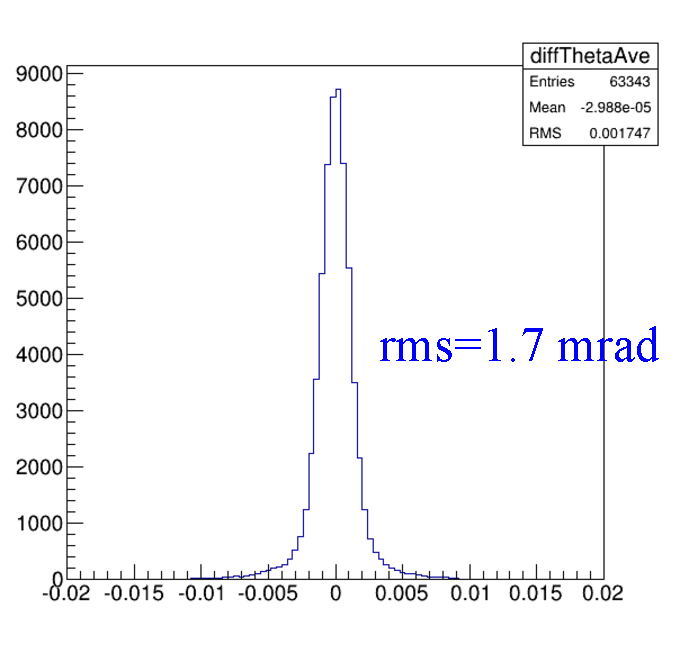
\includegraphics[width=0.45\textwidth]{algorithms-saclay/SaclayResolution.pdf}
  \caption{ $\theta$ resolution at the muon spectrometer entrance.}
  \label{fig:SaclayResolution}
  \end{figure}

 %%%%%%%%%%%%%
\textbf{Calculation of the $x$-coordinate} : What still has to be done is the calculation of the $x$-coordinate using the stereo strips and the firmware implementation. The $x$-coordinate will be used to determine the $\phi$ angle of the particle in order to build the Region of Interest characterized by
 $(\Delta\eta,\Delta\phi)$. This calculation has not been performed in this study because the stereo strips were not implemented in the simulated
samples. However, the formula that should have been used for this calculation is:
 $$\Delta X= \frac{Y_{U}-Y_{X}-\Delta Y_{\theta}}{\tan(\phi_{0})}$$
 where $Y_{U}$ is the average between the two $y$-coordinates of the hit strips of the two layers $U$, $Y_{X}$ is the average between  the two layers of one pair $X$, $\phi_{0}$ is the stereo angle ($\phi_{0}=1.5$ $^{\circ}$). The term  $\Delta Y_{\theta}=~(Z_{U}-Z_{X})\times \tan(\theta)$ (with $Z_{U}$ the average between the two $z$-coordinates of the hit strips of the two layers $U$,  $Z_{X}$ of the two layers $X$, and $\tan(\theta)$ the average of the slopes of the six pairs). This calculation, done for the four $X$ pairs once with the $U$ pair and once with the $V$ pair allows to determine the $x$-coordinate of the hits on each layer.

%%%%%%%%%%%%%%%%%%%%%%
 \subsubsubsection{Summary}
%%%%%%%%%%%%%%%%%%%%%%
The proposed algorithm for the MicroMegas New Small Wheel trigger processor, based on the Look Up Table optimization and strengthen with electronic tests, has an intrinsic efficiency of more than 99\% and can detect a particles with a precision better than 2\,mrad on the polar angle, which fulfill the requirements for the trigger. The construction of the Region of Interest of a track is still to be implemented to check if the total response time is less than 100\,ns.

The algorithm has still to be tested in presence of background which both increases the efficiency and the apparition of fakes, i.e.\ detection of muons that are in reality other products of the collision. The system of pairs should filter the background because the detection of one hit is confirmed by the hit four layers farther, and the fake particles have trajectories that are not geometrically compatible with the LUT content. However, the ionization problem and the intrinsic resolution of the detector are some limitations of the background rejection.

Recently, we have started activities on the production of cavern background simulation. This simulation can be performed using two different
approaches: one is fully based on GEANT\,4, the second is using FLUGG. Both were used in the past for simulation of physics events.
The second approach is currently under validation and the samples are expected to be produced in the next two months.

\FloatBarrier

%-------------------------------------------------------------------------------
\subsection{sTGC Trigger Algorithm}
\label{sec:algorithms-stgc}
% Description, implementation, alignment corrections, performance and latency

\subsubsection{The pre-trigger from the pad towers}

The sTGC trigger is based on determining track coordinates from the centroids of strip charges.
Transmitting $\approx$280,000 strip charges off-detector would requires bandwidths not practical for today's optical interconnect technology.
To reduce the amount of data sent to the off-detector Trigger Processors,
the sTGC uses an 8-fold coincidence along detector pads towers to identify regions where a possible muon candidate has passed.
See Figure\,\ref{fig:LL_PadSelect} and Ref.\cite{padTower}.
Information only from sTGC strips passing through the tower selected by the Pad Trigger is transmitted off-detector to the Trigger Processor.

\begin{figure}[h]
  \centering
  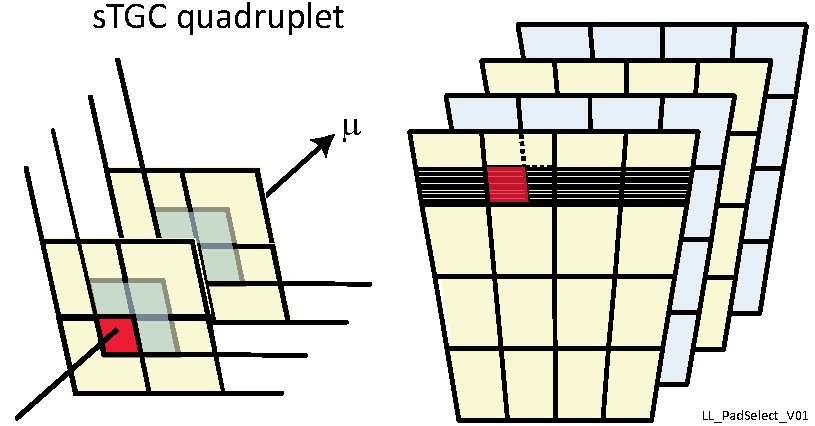
\includegraphics[width=0.55\textwidth]{figures/LL_PadSelect_V01.pdf}
  \caption{The Pad Trigger selects the strips passing through a pad tower made from a coincidence of overlapping pads. One layer of the selected strips is shown.}
  \label{fig:LL_PadSelect}
\end{figure}

It is expected that sometimes a layer of strips will not be useable because its cluster of strips is very wide
due to a $\delta$-ray or neutron, or its signals are saturated due to a neutron track, or the detector layer has become defective.
The algorithm described below discards such clusters and defective layers.
There are enough layers that precise centroids can none-the-less be calculated with less than the full four layers of a quadruplet.

An important parameter is the number of track segments expected to be found,
given the rate of background tracks that successfully pass through all layers of the NSW and could trigger the Pad Trigger.
An estimate of the probability of 1, 2, and 3~segments in a sector is shown in Figure\,\ref{fig:DL_segRates}.
See Ref.~\cite{LellouchRates} for details of the calculation and assumptions.
The planned sTGC trigger path supports transfer of the strip data for up to four track segments.
The figure shows that the losses from this limit are negligible.

\begin{figure}[h]
\centering
   \includegraphics[width=.55\textwidth]{figures/DL_segRates_V01.pdf}
   \caption{Left: The fraction of BCs with one segment (candidate) for each of the three quadruplets.
           Right: The fraction of BCs with one, two, and three segments in a sector. From Ref.~\cite{LellouchRates}}
   \label{fig:DL_segRates}
\end{figure}

\subsubsection{Finding track segments and calculating their parameters}

The sTGC algorithm calculates the $\Delta\theta$, $\phi$ index and R\,index of a track segment.
The algorithm input is an active band of strips for each of the 8~layers.
The information of a band consists of 17~strip ``charges'' measured by the 6-bit flash ADC in the VMM front end ASIC.
The 17~strips include 13~strips of the band itself plus two strips from each of neighboring bands
that provide for charge spreading to adjacent bands.
First, the centroid for each of 8 layers is calculated using the FPGA's built-in DSP (Digital Signal Processing) blocks.
Figure\,\ref{fig:JN_CENTROID_algorithm} shows the centroid calculation algorithm for a single layer.

\begin{figure}[h]
   \centering
   \includegraphics[width=0.9\textwidth]{figures/JN_CENTROID_algorithm_V02.pdf}
   \caption{The centroid algorithm for a single layer, total latency of 8 clocks (320\,MHz)}
   \label{fig:JN_CENTROID_algorithm}
\end{figure}

\FloatBarrier   %%%% recheck need

\vspace{8mm}

Two separate configurable thresholds are provided, one for filtering the input strip signal
and another for defining the signal width in number of strips.
A valid strip band is defined as a band that has one to five active strips,
in all other cases the layer centroid calculation result will have a ``width valid'' flag set to zero.
When ``width valid'' flag of a layer is zero, this layer does not participate in further calculations.

A local center of mass is calculated from the five values in the 5-strip window.
The calculation formula is a weighted mean:
$\frac{\sum_{n=1}^{5} n \times Q_n}{\sum_{n=1}^{5} Q_n}$.
The band's global offset comes from the band-id, i.e.\,the row index of the active pad tower,
and is added to the local-to-band calculation result. Layer centroid calculation algorithm's latency is 8~clocks (320\,MHz).

For both of the 4-layer quadruplets, a centroid is calculated as an average of its valid layer centroids.
This is shown on Figure\,\ref{fig:JN_QCENTROID_algorithm}. Quadruplet centroid calculation latency is 3~clocks (320\,MHz).

\begin{figure}[h]
   \centering
   \includegraphics[width=0.72\textwidth]{figures/JN_QCENTROID_algorithm_V02.pdf}
   \caption{Calculation of the quadruplet centroid, total latency of 11 clocks (320\,MHz)}
   \label{fig:JN_QCENTROID_algorithm}
\end{figure}

%\clearpage
It is possible that during the algorithm execution it is found that there is only one valid quadruplet centroid (i.e.\ it has at least one valid layer centroid).
This situation occurs, for example, when the track passes through the frame of one of the quadruplets.
In this case we use the coordinates within this valid quadruplet to calculate a $\Delta\theta$, albeit with much poorer accuracy.
In order that the algorithm have the same latency in either case,
the low quality result for each of the quadruplets is calculated in parallel to the main algorithm.
If the main algorithm, fails one of the low quality results maybe used instead.

Having the pivot quadruplet centroid value allows the algorithm to define a range for the valid values of the confirmation quadruplet centroid.
A valid range for the confirmation quadruplet centroid value is defined by the maximum deviation of $\pm$15\,mrad from the infinite momentum track angle
as shown in Figure\,\ref{fig:JN_DeltaTheta}.
The maximum allowed deviation, $\Delta\theta_{cut}$, is configurable.

\begin{figure}[h]
   \centering
   \includegraphics[width=0.97\textwidth]{figures/JN_DeltaTheta_V02.pdf}
   \caption{Definition of the valid range of the confirmation quadruplet centroid values, i.e.\ within $\Delta\theta_{cut}$}
   \label{fig:JN_DeltaTheta}
\end{figure}

The $\Delta\theta$ margins LUT defines valid RB (quadruplet B centroid) value ranges for each possible RA (quadruplet A centroid) value.
Each range maps RB onto one of the valid values of $\Delta\theta$; out-of-range values of RB are marked by setting ``valid'' flag to zero.
Figure\,\ref{fig:JN_DeltaThetaBlk} shows a block diagram of the $\Delta\theta$ calculation path.

\begin{figure}[h]
   \centering
   \includegraphics[width=0.95\textwidth]{figures/JN_DeltaThetaBlk_V02.pdf}
   \caption{The Look-up-Table scheme for producing $\Delta\theta$ within the desired cut}
   \label{fig:JN_DeltaThetaBlk}
\end{figure}


R index is a trajectory projection on a Big Wheel and is calculated directly from RA and RB values using mapping conversion LUTs,
as shown on Figure\,\ref{fig:JN_RindexCalcBlk}. Calculation of $\Delta\theta$ and R index is done in parallel with latency of 3 clocks (320\,MHz).



\begin{figure}[h]
   \centering
   \includegraphics[width=0.75\textwidth]{figures/JN_RindexCalcBlk_V02.pdf}
   \caption{Calculation of the R\,index}
   \label{fig:JN_RindexCalcBlk}
\end{figure}

\vspace{-3mm}
\paragraph{Latency and FPGA resources needed}
The total latency for the sTGC algorithm is 18 320\,MHz clocks, including 14 for the algorithm itself plus four more for preparation of inputs and outputs.
One segment finder consumes 1.2\% of the FPGA Virtex\,7~690T LUT resources, 9\% of the Block RAMs and 1.8\% of the DSPs.
This allows ample resources to add two single quadruplet segment finders and the misalignment correction calculator, all replicated four times.
The ancillary functions must also be added.

%\begin{figure}[h]
%   \centering
%   \includegraphics[width=0.97\textwidth]{figures/JN_DeltaThetaBlk_V02.pdf}
%   \caption{The Look-up-Table scheme for producing $\Delta\theta$ within the desired cut}
%   \label{fig:JN_DeltaThetaBlk}
%\end{figure}
%
%
%\begin{figure}[h]
%   \centering
%   \includegraphics[width=0.97\textwidth]{figures/JN_RindexCalc_V02.pdf}
%   \caption{Calculation of the R\,index}
%   \label{fig:JN_RindexCalc}
%\end{figure}

\FloatBarrier

\subsubsection{Compensating for misalignments}

The sTGC algorithm provides quadruplet misalignment correction for the cases that are shown in Figure\,\ref{fig:DL_misalignment}:
\begin{enumerate}\itemsep-6pt
\item[(1)] displacement along r-axis (axis orthogonal to the beam axis),
\item[(2)] displacement along the z-axis (beam axis),
\item[(3)] rotational displacement around the detector edge orthogonal to the r-axis,
\item[(4)] rotational displacement around the r-axis
\item[(5)] rotational displacement around the axis parallel to the z-axis.
\end{enumerate}

\begin{figure}[h]
   \centering
   \includegraphics[width=0.2\textwidth]{figures/DL_misalignment_V01.pdf}
   \caption{The possible misalignments of a sTGC quadruplet}
   \label{fig:DL_misalignment}
\end{figure}

Each of the six quadruplets of a sector are divided into sections by band-ID and $\phi$-ID.
For each of these sections, four constant geometrical parameters ($dr$, $dr^{2}$, $dr d\phi$, $d\phi$) are stored in six 2-D look-up tables.
Each cell of the LUT contains a set of the four values for each combination of band-ID
(or predefined contiguous set of band IDs) and $\phi$-ID (or predefined contiguous set of $\phi$-IDs).
Five measured mechanical alignment values for each of six quadruplets of a sector are stored in a RAM and updated by the calibration process.
The total correction offset for one quadruplet is calculated as a dot product of the two entries.
This misalignment calculation, as shown on Figure\,\ref{fig:JN_misalignment_correction},
is done in parallel with the layer centroid algorithm and is added to its result, i.e.\ one additional (320\,MHz) clock latency.

\begin{figure}[h]
   \centering
   \includegraphics[width=0.9\textwidth]{figures/JN_misalignment_correction_V02.pdf}
   \caption{LUT-based misalignment correction algorithm. Numbers in orange represent the possible chamber misalignment cases according to Figure\,\ref{fig:DL_misalignment}.}
   \label{fig:JN_misalignment_correction}
\end{figure}

\FloatBarrier



\FloatBarrier

%-------------------------------------------------------------------------------
%\subsection{Candidate Selection}
%\label{sec:algorithms-selection}
%\input{inputs/algorithms-selection}
%\FloatBarrier

%-------------------------------------------------------------------------------

%-------------------------------------------------------------------------------
\section{Trigger Processor Hardware Platforms}
\label{sec:hardware-platforms}
There are two candidates for the NSW Trigger Processor hardware platform.
One option is based on the boards for the \PhaseOne LAr Trigger system upgrade~\cite{hardware-LAr-Carrier,hardware-LAr-OTC} and the other is based on SRS boards designed within the RD51 collaboration~\cite{hardware-SRS-Carrier,hardware-SRS-Mezz}.
The trigger signals will be processed in TP mezzanine cards~\cite{hardware-LAr-OTC,hardware-SRS-Mezz}
mounted on ATCA carrier boards~\cite{hardware-LAr-Carrier,hardware-SRS-Carrier}. The LAr mezzanine card is a card with standard AMC interface, while the SRS mezzanine has a custom interface.
There are four LAr mezzanine cards per ATCA board but only two SRS mezzanine cards.
The custom interface allows the SRS mezzanine card to have a large number of faster interconnects between FPGAs.
The four documents above describe the boards in detail while this
section compares both options and provides a selection criteria.

All boards are based on Xilinx Virtex FPGAs. The two mezzanine card options use FPGA
Virtex 7 footprints compatible with XC7VX415T, XC7VX485T, XC7VX550T, XC7VX690T FPGAs~\footnote{The SRS option uses package FFG1158, while the LAr option uses package FFG1927. The difference being on the number of I/O pins but both are sufficient for our needs.}.
At this point, we believe the TP will require the higher capacity XC7VX690T chip, which has GTH transceivers instead of GTX (as in XC7VX485T).


\subsection{Specification Comparison}

\subsubsection{ATCA Standard Interfaces}
\label{atca-standard-interfaces}

Both carrier boards adhere to current ATCA standards and provide all required
interfaces.


\subsubsection{Optical I/O for Detector Data and Sector Logic}
\label{optical-io-for-detector-data-and-sector-logic}

It is required that each Trigger Processor must be capable of operating
independently of the other as well as in the normal operating mode of
MM/sTGC pairs in tandem. Each TP must therefore be capable of driving
sufficient number of fibers to the Trigger Logic. That requirement is
two independent channels to carry up to four trigger candidates each, as
well as a 7-fold fan-out to accommodate up to seven Sector Logic boards. Thus,
each TP requires 14 fiber outputs running at \textgreater{}6.4\,Gbps
each. Each TP also requires 32 fiber inputs to accommodate one sector
for either the MM or sTGC. For the MM\_TP, input bandwidth of 6.4\,Gbps
is required. A fiber link to FELIX for TTC, Level-1 data and
monitoring/configuration data is also required.

\begin{description}
\item[SRS mezzanine card]
The SRS mezzanine card provides three Avago $\mu$Pod optical transmitter modules and
the same number of receiver modules. Each module has 12~channels which
are specified to operate at up to 10\,Gbps, for a total of 36~channels
each of transmitters and receivers.

\item[LAr mezzanine card]
The LAr mezzanine card has standard AMC interface.
It provides 4x each Avago $\mu$Pod transmitter and receiver
modules for a total of 48 i/o channels. For use in the NSW Trigger
Processor, only three each of the transmitter and receiver modules would
be populated, for a total of 36 i/o channels. Data rates of
\textgreater{}10 Gbps have been demonstrated on the LAr card as this is
a requirement for operation in the LAr detector.
\end{description}


\subsubsection{Mezzanine to mezzanine lateral communication}
\label{amc-to-amc-lateral-communication}

Each \MM TP must transfer its track-segment candidates to the neighboring \stgc TP
within one bunch crossing. At least up to eight candidates must be transferred in that time.
Each transfer requires 21 bits of data per candidate plus six for BCID and one overflow indicator
for a total of $21\times8 + 6 +1 = 175$ bits/BC. Thus, aggregate bandwidth for lateral communication between AMC cards is 175/25ns = 7.0\,Gbps.

\begin{description}
\item[SRS mezzanine card]
The SRS mezzanine card provides two independent Trigger Processors per card,
with one dedicated to \MM and the other to \stgc. Each has its own
FPGA and there are 64 LVDS pairs connecting the two. To transmit the
required hit data from \MM to \stgc using all 64 lines, each would have to
run at 100\,MHz. Since the two FPGAs are within \textasciitilde{}10\,cm of
each other and on the same board, speeds beyond \textasciitilde{}1\,Gbps
should be easily achievable. As the SRS mezzanine card is still in
development, it is not available for testing at this moment.

\item[LAr mezzanine card]
Each mezzanine card will be configured as a \MM TP or as a \stgc TP. The FPGA on
each card has, at the present time, eight LVDS lines which are transmitted
to the ATCA carrier card through a connector. The LVDS output lines from
one \MM mezzanine connect to an FPGA on the ATCA carrier, are transferred to
corresponding LVDS outputs on that FPGA, and then to the \stgc mezzanine
through its connector. Thus, the LVDS lines travel from \MM mezzanine to the
\stgc mezzanine through two mezzanine connectors and an FPGA. Bandwidth for this
arrangement has been tested to \textasciitilde{} 600\,Mbps, but without
the intervening FPGA present. The designers plan to test to
\textgreater{}1\,Gbps and are confident they can achieve higher bandwidth
than has been demonstrated at present. For present purposes, a
comfortable operating speed for these connections of 500\,Mbps is assumed
until higher rates have been verified.

The present iteration of the mezzanine (called OTC for Optical Test Card) has
eight such LVDS pairs. At 500\,Mbps each, aggregate bandwidth is 4.0\,Gbps
which is sufficient for transferring up to five trigger candidates per BC
but not eight. The LAr AMC designers will attempt to expand the number of
LVDS lines in subsequent iterations to accommodate the required
bandwidth. At currently achieved bandwidth, a minimum number of LVDS
lines in future board iterations would be 16, with slightly more being
desirable.
\end{description}


\subsection{Selection Criteria}\label{selection-criteria}

The main difference between the platforms appears to be one of topology.
The LAr platform has four independent and identical AMC cards which can
implement one trigger processor of each flavor. The two cards need to
communicate laterally through the ATCA card and, at the moment, there
are only 8 LVDS lines available for that purpose. These have been tested
to 600\,MHz and perhaps can go higher. The designers may also be able to
increase the number of lines to 16, thus enabling operation at a lower
clock frequency. Assuming that the required lateral bandwidth can be
achieved, it is unlikely that operation could be extended to higher
rates of hit candidates.

The SRS implements the system with ``double wide'' mezzanine cards with the
two flavors of trigger processor on each and 64 LVDS pairs between them.
Each can be expected to operate at \textasciitilde{}1\,GHz which is
significantly higher than required for 8 hit candidates per BC and there
would be no problem extending that to significantly higher throughput.
The mezzanine board design and layout has been completed, however, it has not yet
been produced, so there is no module in existence yet for testing.

The ATCA-SRS board (Virtex 6) is already available and it was tested extensively within the RD51 collaboration. The next version of the board, which will likely use a Virtex 7 FPGA, is now being designed and is expected in mid 2015. This upgrade is not likely to be necessary for the TP project given the little functionality of the carrier card.
The LAr ATCA carrier board has just finished the design stages. Since it is needed for the LAr trigger system, there should be little doubts that a card will eventually be available.

The LAr platform will need additional design/fabrication
cycles as will the SRS. Given that, the selection would require that development time be
allowed before the decision is finalized. The decision should only be taken once we have tested the first prototype from both systems.

A few selection criteria items are:
\begin{itemize}
\item The major selection criteria lays with the ability of either platform to
deliver the required lateral bandwidth of 7.0\,Gbps or higher for upgrades.
Having enough bandwidth to transmit more information within one BC for a possible more complex trigger algorithm in \PhaseTwo is desirable.

\item Support that can be expected for additions or correction of design errors that may be required. The LAr system will be supported by Stonybrook and assurances from US ATLAS are required to ensure that they will get any needed budget support. The SRS system will be supported by a combination of Bucharest and the commercial company that is selling the system. The details must be clarified.

\item Although detailed costing has not yet been done, the costs of the two solutions should be comparable, since it is dominated by the cost of the FPGA and electro-optics. However the effect on cost due to the commercialization needs to be clarified.
\end{itemize}


It should be stated that the selection of the hardware platform is not yet on the critical path.
Algorithms and the ancillary functions are being developed using evaluation boards from Xilinx and Hitech Global.
The Xilinx boards have four bidirectional links, the Hitech Global has 24.





%-------------------------------------------------------------------------------

%-------------------------------------------------------------------------------
\section{Testing}
\label{sec:testing}
The testing of the trigger processor and algorithm
implementation in hardware, for both \MM and sTGC, will be
performed in four ways. Initially, signals from upstream electronics
are generated in the trigger processor FPGA and looped back in
order to test the implementation of the algorithm in hardware. Testing of the full
electronics chain requires further work. In
the absence of realistic chambers, the
detector and front-end output will be emulated by pattern generators
in order to characterize the full trigger chain, including
the ADDC. Additionally, the trigger
system will be tested on real detectors with cosmic rays and in a
test beam.
%-------------------------------------------------------------------------------
\subsection{Initial Testing of the MM Implementation}
\label{sec:testing-mmTrigProcImp}
A slice containing all of the elements of the Trigger Processor
design has been implemented with no timing errors and is being tested using a Xilinx VC707
Development board. This board includes a Virtex XC7VX485T-2FFG1761C
FPGA. The implementation includes two ADDC GBT interfaces and associated
trigger processor algorithm.  We are currently working on the timing closure of a full design.

To exercise the trigger processor design we have developed an evaluation board based ADDC
emulator. This design can be used to supply properly formatted ADDC
GBT packets through an optical transmitter as sent from an actual
ADDC. The same ART data used for simulations is being used for hardware
testing. We are also generating pseudo random ART data to test the
GBT communication and timing of packet decoder. A block diagram of the data flow  can be seen in Figure~\ref{fig:artDataStimAE}.

\begin{figure}[h]
 \centering
 \includegraphics[width=0.7\textwidth]{figures/testing/artDataStimAE.pdf}
 \caption{Initial testing configuration using an ADDC emulator}
 \label{fig:artDataStimAE}
 \end{figure}

To evaluate the hardware implementation, we compare the hardware results
with results generated using a computer simulation of the algorithm. The initial testing of the hardware has shown the entire algorithm is working functionally.  There are some differences between the hardware and software results due to the number of significant bits used in the hardware.  It is likely we will want to increase the precision used in some of the hardware calculations. We expect this would increase the latency by roughly 6 to 9 ns.   Since the calculations are done in an area of the implementation that has a low multiplication factor, increasing the precision will have a low impact on the resources used. 


We have begun integration testing with the BNL ADDC and have successfully
transmitted data to the Trigger Processor using the ADDC's VTTx ASIC.


%-------------------------------------------------------------------------------
\subsection{Pattern Generators}
\label{sec:testing-pg}

\subsubsection{The Micromegas ART Pattern Generator}

In order to properly test the full trigger electronics chain without
access to a large number of chambers, it is necessary to implement a
pattern generator  to simulate the ART (address in real time) output
from the VMM chips. This pattern generator will interface with the
ART Data Driver Card (ADDC), which will then transmit information via
fiber optic link to the Trigger Processor (TP).

The firmware for the ART Pattern Generator (APG) has been written and
is currently being tested on a Xilinx
Virtex 7 FPGA in a VC707 development board. Each development board has
FMC output connectors. A mezzanine
card has been developed to adapt these FMC connectors to the MiniSAS
connectors expected by the ADDC card.

The signal emulation will be accomplished by reformatting simulated
muon events in the NSW in Athena and sending them via an ethernet
interface to the FPGA. On the FPGA, the hits will be sorted to the
correct ART output and clocked out according to the timing indicated
in the event. Finally, the 6 bits of the strip number are output
serially through the FMC connector according to the LVDS standard
expected by the ADDC inputs. Figure~\ref{fig:artDataStimPG} shows the
general chain of the testing configuration using the APG and 
Figure~\ref{fig:APGBlockDiag} shows the full program flow of the APG from simulation to serialized output on the evaluation board FPGA.

\begin{figure}[h]
 \begin{center}
 \includegraphics[width=0.9\textwidth]{figures/testing/artDataStimPG.pdf}
 \caption{Testing configuration for APG.}
 \label{fig:artDataStimPG}
 \end{center}
 \end{figure}

\begin{figure}[h]
 \begin{center}
 \includegraphics[width=0.9\textwidth]{figures/APGBlockDiagramFinal}
 \caption{Block diagram representing the detailed flow of the APG.}
 \label{fig:APGBlockDiag}
 \end{center}
 \end{figure}

The APG will be used in conjunction with the BNL ADDC and the trigger
processor to test the performance of the electronics and trigger
algorithm  as a function of various parameters of interest (including
track slope,  hit rates, etc.). Performance metrics for the algorithm
will include efficiency and fake rates. Performance metrics for the
electronics  will include latency measurements and stress tests with
large track and/or background rates.
\FloatBarrier

\subsubsection{The sTGC Pattern Generator}
\label{sec:sTGCpattern}

A Matlab program generates patterns for testing the sTGC algorithm.
Values for track angle, hit radius, hit intensity and hit $\phi$ position are taken from a uniform distribution within predefined limits.
The event parameters are then parsed into Trigger Processor algorithm inputs for each of the eight layers.
Figure\,\ref{fig:TGCevgen} shows a graphical representation of one quadruplet image of one generated event.
The expected algorithm output is calculated for each generated event for verification.

\begin{figure}[h]
   \centering
   \includegraphics[width=0.8\textwidth]{figures/JN_TGCevgen_V01.pdf}
   \caption{An image on the background showing an active pad tower (defined by the overlapping pads shown in grey) as a dark square,
   where the dots indicate which of the layers in the pad tower have pad signals above threshold.
   The foreground image shows the pulse heights of the strips passing through the pad tower for this event.}
   \label{fig:TGCevgen}
\end{figure}

This mechanism was implemented on two identical sTGC trigger demo FPGA boards.
One board emulated the detector outputs using preloaded generated event data patterns for several events and the other was configured as the Trigger Processor.
In the next step towards algorithm testing,
simulated muon events from the ATLAS simulation program will be parsed into the sTGC Trigger Processor input pattern.
This will allow verification of the algorithm functionality and its optimization.
Using the same simulated events will also allow comparison between sTGC and \MM trigger processing algorithms.
As a final test, playback pattern generation will be employed in which real event data can be recorded and parsed as an input pattern.

\FloatBarrier



%-------------------------------------------------------------------------------
\subsection{Cosmic Ray Testing}
\label{sec:testing-cosmics}

%{\bf Need some info about cosmic ray stand at Weizmann. }

With real detectors it will be possible to do more detailed
testing of the trigger processor. Testing with cosmic rays is an
important aspect of the trigger testing
plan. A cosmic ray test stand is not subject to test beam schedules,
allowing for rapid iteration and debugging in the early stages of
development. This is especially important because it allows both the
MM and sTGC systems to debug the interface with a real VMM chip.
Thus, part of the testing plan is to assemble realistic detector
prototypes for the MM and sTGC and place them in
cosmic ray telescopes.

It is important to ensure that
the cosmic ray muons used have sufficient momentum ($\mathcal{O}$\,(1\,GeV)) so as
to avoid the effects of multiple scattering. Additionally, it is useful
for the cosmic ray test setup to have a large angular acceptance, a
good angular resolution, and good timing resolution to allow precise
characterization of the trigger's behavior. Such test setups are
available at Harvard for the MM chambers and Weizmann for the sTGC
chambers. The test stands will include small-scale realistic detector setups,
including a small assembled MM octuplet and and two sTGC quadruplets.

The Harvard cosmic ray test setup consists of three planes of
scintillators sandwiching a 2\,m thick concrete block. It can detect
cosmic ray muons of greater than 0.8\,GeV with a time resolution better
than 1.5\,ns.  It has a coverage of 2.5\,m$^2$, an angular acceptance
of up to 25$^{\circ}$ from vertical and a 1.5$^{\circ}$ angular resolution.

The Weizmann test stand is designed to hold up to two 60\,cm $\times$ 40\,cm quadruplets.
A VMM configuration system was built to configure up to 12~chains of VMM chips.
There is one scintillator above and one below.
The lower scintillator has $\approx$20\,cm of lead shielding between it and the detectors to ensure that only hard cosmic muons are triggered.
The quadruplets were outfitted with VMM1 boards connected to strips and pads. (See Figure\,\ref{fig:WeizmannQuardupletCosmicSetup}.)
The VMM1 trigger outputs were connected via cables to the demonstrator boards mentioned in Section\,\ref{sec:sTGCpattern}.
A dual-VMM2 board was designed to replace the VMM1 boards, but work on it was halted when the trigger outputs of the VMM2 were found to be disabled.
This work will continue with VMM3.


\begin{figure}[h]
  \centering
  \includegraphics[width=0.85\textwidth]{figures/testing/WeizmannQuardupletCosmicSetup.JPG}
  \caption{sTGC quadruplet cosmic test setup. Shown a connection of two layers of a quadruplet. In each layer
  four VMM1 boards are connected to 64 strips and one VMM1 board (denoted by a black arrow) is connected to 16~pads.
  Other two layers of this quadruplet are connected on the opposite side.}
  \label{fig:WeizmannQuardupletCosmicSetup}
\end{figure}

\FloatBarrier

Once the realistic detector setups are assembled, the ultimate goal is to test the full
trigger chain with the chambers. First, the chain will be
tested with the trigger processor still in the evaluation board
platform, mainly testing the full communication pathway from chamber readout
to trigger processor. Once this is found to be working, the trigger
processor will move to its eventual home on the hardware platform in
an ATCA crate. There, more detailed tests with the cosmic rays can be
performed, including full measurements of the latency, trigger
efficiency, and hit throughput. Additionally, tests for the signal
integrity and bit errors through the whole electronics chain can be
done.

The key asset of the cosmic ray test setup is to be
able to iterate rapidly and debug issues that may arise without having
to wait for beam in a test beam setting.







%-------------------------------------------------------------------------------
\subsection{Vertical Slice and Test Beam}
\label{sec:testing-vertical-slice}
%{\bf Add information about the vertical slice at CERN and eventual
%test beam studies}

In order to integrate the various components of the NSW electronics,
a vertical slice of the system will be assembled in a lab on the Meyrin site.
It will include prototypes of all components from VMMs through the Trigger Processors, ROD and an evaluation board to capture the Sector Logic input.
The slice can be used to playback captured and simulated data, injected at various points.
Unlike beam and cosmic ray tests, it will allow testing the Trigger Processors at the 40\,MHz bunch crossing rate.

Part of the testing strategy for the Micromegas trigger includes
the installation of the Micromegas Small Wheel (MSW) in the ATLAS
cavern.
This will allow the Micromegas trigger to be tested with low-level cavern background conditions.
The electronics chain for the MSW will
include the VMM2 readout chip and the ADDC card for transmitting ART
signals to an evaluation board located in USA15. The evaluation board
will receive the ART signals from the ADDC and decode them. On an
ATLAS Level-1 Accept, the evaluation board will format all of the ART
data within four bunch crossings of the ATLAS trigger and send them to
the ATLAS DAQ system via ethernet. Events will also be sent via a second ethernet
link to a desktop PC to allow for real time monitoring. Recording the
data in this way will allow for testing of the trigger algorithm and
implementation using ART data from Micromegas with some cavern background.
The trigger algorithm for segment reconstruction can be implemented in the evalaution board and recorded.
The collected ART data can also later be replayed through existing pattern
generators to allow for quick debugging of the trigger electronics,
offering a set of tests different from those generated by Athena.
Figure\,\ref{fig:MSWChain} shows the trigger chain envisioned for the MSW.

\begin{figure}[h!]
 \centering
 \includegraphics[width=0.9\textwidth]{figures/MSW_Trigger}
 \caption{MSW trigger chain proposal}
 \label{fig:MSWChain}
 \end{figure}


\FloatBarrier
%-------------------------------------------------------------------------------

%-------------------------------------------------------------------------------
\section{Phase-2 Compatibility}
\label{sec:phase2}
The current latency budget for the Phase\,1 trigger processor for the
New Small Wheel, and the forward muon system in general is extremely
tight.
While the NSW trigger as designed now for installation in Long Shutdown\,2 (LS2)
already meets the Phase\,2 requirement of an angular resolution of 1\,mrad,
it is quite possible that one may further lower the thresholds
for muon momentum by taking advantage of the increased Level-1 latency time
to do a more refined calculation of muon pointing and momentum, or to
improve robustness and redundancy, e.g.\ in case of missing layers.

Currently, prompt signals from the Micromegas detectors and sTGC are
used to form track segments in the NSW. A cut is made on the pointing
back to the interaction region in a set of trigger processors, and the
resulting $\Delta\theta$, and RoI information is transmitted to the Sector Logic
which looks for a coincidence with prompt signals from the Big Wheel.
Currently, the latency budget for the NSW trigger processor algorithm
is approximately 100\,nsec, when fiber optic delays, serialization,
deserialization and other factors are taken into consideration, along
with the processing and transmission time associated with the Sector
Logic.

With a much larger amount of latency available in Phase\,2, and
anticipated advances in FPGAs, it makes sense to seriously consider a
more powerful trigger processing scheme that can take advantage of
additional processing time to make a much more refined trigger
algorithm. In this case, the Phase\,1 trigger processor hardware (ATCA cards + mezzanines),
excluding the ATCA crates and optical fibers, would be replaced.
Since such proposal is for equipment in USA\,15, it has
little to no impact on the current plans, but can provide for the
possibility of a much more refined Level-1 trigger that should be capable
of pushing down the momentum threshold for forward muons significantly
by including more fine-grained information available, given the
latency.
%-------------------------------------------------------------------------------

%-------------------------------------------------------------------------------
\section{Project Organization}
\label{sec:organization}
The NSW Trigger Processor project is being carried out by a working group coordinated by 
Jo\~{a}o Guimar\~{a}es da Costa. The working group activities are integrated in the NSW Electronics group coordinated by Lorne Levinson.
The group consists of institutes that have been involved in building the current muon trigger system and new institutes. There are several physicists and engineers that have already contributed to the project and more are joining now. The following sections cover the commitment and responsibilities of the participants.
% and the current schedule. 

%-------------------------------------------------------------------------------
\subsection{Responsibilities}
\label{sec:responsibilities}
The NSW Trigger Processor project is being carried out by a collaboration of several ATLAS institutions. The project is comprised of four major aspects: the hardware platform, the firmware, trigger studies and testing. The hardware area also includes the input and output fibers.
The firmware is divided into the trigger algorithm and ancillary functions.
Whenever feasible tasks are common to the MM and sTGC technologies.
Below is an organigram of the different tasks with the corresponding manpower.
This is a snapshot of the current situation and how we expect the manpower to evolve in the near future.
Physicists\,(P) include senior and postdoc level staff, while engineers\,(E) and students\,(S) are listed separately. The estimated full-time equivalent commitment for each individual is also indicated.

Work to be done during the final installation at CERN is not included in this graph. It is expected that much of the manpower listed here will eventually transition to those tasks.


\begin{figure}[h]
    \begin{center}
        \includegraphics[width=0.95\textwidth]{figures/JG_Organigram_TP-v01.pdf}
        \caption{Organization and manpower dedicated to the Trigger Processor project, including engineers\,(E),  physicists\,(P) and students\,(S). The full-time equivalent estimations for each individual are also provided.}
        \label{fig:organigram}
    \end{center}
\end{figure}

\paragraph{Hardware}
\begin{description}
\item[LAr Hardware Platform] The LAr AMC-format Optical Test Card was designed by BNL, Stony Brook and Arizona for the LAr trigger upgrade. The card was not adopted by the LAr trigger project although prototypes exist and they are fully functional and tested. This card could fulfill the requirements of the TP but it requires updates to increase the bandwidth communication between mezzanine cards. The corresponding ATCA carrier board is designed and it will be used by the LAr trigger. It also requires updates to increase the inter-mezzanine bandwidth. Stony Brook and Arizona will design and implement the modifications required for the muon trigger project. Only this effort is indicated in Figure~\ref{fig:organigram}.
It includes 0.35 FTE enginnering for design updates to the boards and firmware, 0.1 FTE engineering for production hardware testing, 0.1\,FTE labor for production hardware testing and 0.1 FTE for technical oversight.

\item[SRS Hardware Platform] The ATCA-SRS carrier board was designed within the RD51 Collaboration and it is already available. An update is planned for mid-2015 but not deemed essential for this project. The ATCA-SRS Carrier Board is being manufactured under a licensing contract between Eicsys Gmbh, Germany licensee and the IP Holder Consortium within RD51 collaboration (CERN, IFIN-HH and Polytechnic University of Valencia), as licensor. The licensing contract is not exclusive.

The High-Density Optical Receiver (HORX) mezzanine board is a responsibility of IFIN-HH, Bucharest. Its design and realization is being done by an external specialized company (Samway Electronics, Bucharest). The final design is part of the contracted deliverables; therefore all design sources are in possession of IFIN-HH~\cite{hardware-SRS-Mezz}.

Apart from the two companies mentioned, which will provide support for the two boards, the following IFIN-HH team will be in charge of the design, specifications and firmware \& software support: Sorin Martoiu\,(0.2 FTE), Research Engineer; Michele Renday, Graduate Student\,(0.1\,FTE); and Gabriel Stoicea, Physicist\,(0.1\,FTE).


\item[Fiber plant] The Trigger Processor i/o fibers are integrated in the fiber plant (Appendix~\ref{app:specs-fibers}) that is the responsibility of the Weizmann Institute.
\end{description}

\paragraph{Firmware} includes algorithms and ancillary functionality firmware development. The bulk of the resources for firmware testing is included in the ``trigger studies and testing'' item.
\begin{description}
\item[MM Fitter Algorithm] The algorithm has been developed by the Harvard group. Previous contributions have been made by the postdoc and students listed under trigger studies in Figure~\ref{fig:organigram}. The same team will continue supporting the algorithm. Moving forward the algorithm firmware will be done by Nathan Felt (0.5\,FTE) with support from students and oversight from John Huth and Jo\~{a}o Guimar\~{a}es.
\item[MM Look-Up-Table Algorithm] The algorithm has been developed by the Saclay group, with contributions from Samira Hassani, Hevré le Provost, Claude Guyot and Philippe Schune. The team is being revamped and they are now focusing on the cavern background simulation. More contributions are expected in the longer term.
\item[sTGC Algorithm] The algorithm has been developed and will continue to be developed by the Weizmann group. The team includes Lorne Levinson and 0.2\,FTE of engineering support (Julia Narevicius and Alex Roich).
\item[Ancillary Functionality] Several groups have taken responsibility for delivering the firmware for the ancillary functions. These include Illinois, Weizmann and BNL. The Arizona group will also help, in particular if the LAr platform option is chosen, given that many of these functions are common to the LAr trigger board. The manpower pledged currently includes 0.75\,FTE engineering and 0.2\,FTE of student support. Lorne Levinson and Verena Outschoorn will oversee the project.
\end{description}


\paragraph{Trigger studies and testing} Most of the people currently making trigger studies will also be the manpower for future testing of the trigger hardware, firmware and performance. Given the different timescales both tasks are considered together.
\begin{description}
\item[MM Trigger] The trigger algorithm studies have been done by a small team of students and postdocs. Moving forward this team will be enlarged to include support for the trigger testing at home institutions and at CERN. Harvard, Saclay, BNL and Illinois are expected to contribute with a total of 1.35\,FTE engineering, 0.40\,FTE physicist and 1.5\,FTE student support.
\item[sTGC Trigger] The manpower pledged for the sTGC trigger studies and testing is limited to Lorne Levinson (0.05\,FTE). Although some of the hardware tests will be common with the ones from the MM trigger, this team needs to be enlarged.
\end{description}



\begin{comment}

Saclay: Future????

Saclay team who contributed to the trigger algorithm:
Samira Hassani
Hevré le Provost
Claude Guyot
Philippe Schune


\subsubsection{In the graph}

Stony brook:

Dean and I talked about the incremental manpower we'd need for the R&D  related changes to the AMC and ATCA carrier beyond the work already needed for LAr.   We estimate about 3 months of labor, roughly 1 month for the AMC and 2 months for the carrier.   We'll refine the estimate a bit this week to include incremental labor associated with production.  This will matter for the AMC more than the carrier.

As far as personnel availability goes, the engineer who has been doing the AMC card will basically finish that in the next month or so.   He would then be free to work on the mods for the AMC card.   Either he or Dean would do the layout changes for the carrier.

The original 0.25 FTEs is the engineering needed to make the AMC and carrier design changes to add four AMC ports to make a total of 16 LVDS connections available(primarily layout updates).  We've also now estimated the additional FTEs for testing firmware changes and production testing.  The full list is

0.25 FTE engineering (Chuck Pancake) for design  updates to AMC and carrier
0.1   FTE engineering for updates to LVDS testing firmware (Pancake)
0.1   FTE engineering for production hardware testing (Eugene Shafto)
0.1   FTE off project labor for production hardware testing (post doc, Boline; students)
0.1   FTE off project technical oversight Schamberger/Hobbs



Illinois:
Todd 30\% firmware, 20% testing
Wooyoung 20\% firmware, 20% testing
Verena 5\% firmware, 5% testing, 40% software (I’m not teaching the summer & fall)

Todd Moore
Research Engineer
ancillary functions
testing, including hardware

Wooyoung Moon
Graduate student
firmware development and testing
commissioning, including integration at cern


Weizmann:
Julia Narevicius, Alex Roich, Lorne Levinson (Algorithm development and corresponding firmware implementation, Ancillary functions firmware)
Julia and Alex are each 20\% on NSW TP (and another 20% each on FELIX).

Bucharest:
The following team from our institute will be in charge of the design, specifications and firmware & software support,
Sorin Martoiu, Research Engineer, 20\%
Michele Renda, Graduate Student, 10\%
Gabriel Stoicea, Physicist, 10\%

BNL:
Brookhaven will soon have an Electronic Engineer full time Ph.D. (George Iakovidis) working on
the firmware ancillary TP tasks, test beams and analysis, CERN vertical slice coordination and, eventually, commissioning.

Harvard:
John Huth 15\%
Joao
Nathan 100\% (50/50)
John Oliver 15\% - testing
Possible new student


\paragraph{Hardware platform}
\vspace{-5mm}
\begin{itemize}\itemsep-4pt
        \vspace{-1mm}
	\item LAr Card (option A):
	\begin{itemize}\itemsep-6pt
	    \vspace{-2mm}
	    \item Arizona (\emph{Kenneth Johns})
	    \item BNL
	    \item Stony Brook (John Hobbs)
	\end{itemize}\itemsep-4pt
	\item SRS Card (option B):
	\begin{itemize}\itemsep-4pt\parskip-4pt\parsep-4pt
	    \vspace{-1mm}
	    \item Bucharest (Sorin Martoiu)
	\end{itemize}
\end{itemize}

\paragraph{Algorithm development and corresponding firmware implementation}
\vspace{-5mm}
\begin{itemize}\itemsep-6pt
	\item Harvard
	\item Saclay
	\item Weizmann (Julia Narevicius, Alex Roich, Lorne Levinson)
\end{itemize}

\paragraph{Ancillary functions firmware}
\vspace{-5mm}
\begin{itemize}\itemsep-6pt
	\item Arizona (Ken Johns)
	\item Harvard
	\item Illinois (Verena Martinez Outschoorn, Todd Moore, )
	\item Weizmann (Julia Narevicius, Alex Roich, Lorne Levinson)
\end{itemize}

\paragraph{Testing}
\vspace{-5mm}
\begin{itemize}\itemsep-6pt
	\item Harvard (Tomo Lazovich, Hugh Skottowe, Nathan Felt)
	\item Illinois
	\item Weizmann
\end{itemize}

\paragraph{Software}
\begin{itemize}
	\item Michigan...
\end{itemize}

\end{comment}


%-------------------------------------------------------------------------------
%\subsection{Schedule}
%\label{sec:schedule}
%\input{inputs/schedule}
%-------------------------------------------------------------------------------

%Place your results here.

% All figures and tables should appear before the summary and conclusion
% The package placeins provides the macro \FloatBarrier to achieve this
\FloatBarrier


%-------------------------------------------------------------------------------
\section{Conclusion}
\label{sec:conclusion}
This document describes the current status of the NSW trigger
processor. It documents the specifications, the trigger algorithms
developed and the testing procedures. There are some open issues to be
investigated, including a study of the bandwidth between FPGAs in the
LAr card, the relative mechanical alignment of the BW and NSW and a study of the
expected trigger rates. The choice of the trigger platform hardware, although desirable, is not critical at this point. Studies of hardware/firmware trigger implementation have been hindered by the VMM2 problems.
For simulated data we are dependent on the simulation group.
The Athena simulation of both sTGC and Micromegas triggers is not complete.
The sTGC algorithm studies are especially limited by this absence.


%TO DO:
%\begin{enumerate}
%\item update trigger platform text and selection criteria (Lorne to check)
%\item improve Phase-2 compatibility
%\item Organization section
%\begin{enumerate}
%\item update responsibilities section (need text update)
%\item add schedule
%\end{enumerate}
%\item Algorithm sections
%\begin{enumerate}
%\item check new text from MM
%\end{enumerate}
%\item conclusions
%\end{enumerate}

%Enter conclusions here
%
%\subsection{Open Issues}
%Here is a list of issues that will be
%
%\paragraph{Bandwith between FPGAs in LAr card}
%bla bla
%
%\paragraph{Relative alignment of BW and NSW}
%bla bla
%
%\paragraph{Study expected trigger rates}
%bla bla

%-------------------------------------------------------------------------------

%-------------------------------------------------------------------------------
%\section*{Acknowledgements}
%-------------------------------------------------------------------------------

%% Acknowledgements for papers with collision data
% Version 14-Oct-2014

% Standard acknowledgements start here
%----------------------------------------------
We thank CERN for the very successful operation of the LHC, as well as the
support staff from our institutions without whom ATLAS could not be
operated efficiently.

We acknowledge the support of ANPCyT, Argentina; YerPhI, Armenia; ARC,
Australia; BMWFW and FWF, Austria; ANAS, Azerbaijan; SSTC, Belarus; CNPq and FAPESP,
Brazil; NSERC, NRC and CFI, Canada; CERN; CONICYT, Chile; CAS, MOST and NSFC,
China; COLCIENCIAS, Colombia; MSMT CR, MPO CR and VSC CR, Czech Republic;
DNRF, DNSRC and Lundbeck Foundation, Denmark; EPLANET, ERC and NSRF, European Union;
IN2P3-CNRS, CEA-DSM/IRFU, France; GNSF, Georgia; BMBF, DFG, HGF, MPG and AvH
Foundation, Germany; GSRT and NSRF, Greece; ISF, MINERVA, GIF, I-CORE and Benoziyo Center,
Israel; INFN, Italy; MEXT and JSPS, Japan; CNRST, Morocco; FOM and NWO,
Netherlands; BRF and RCN, Norway; MNiSW and NCN, Poland; GRICES and FCT, Portugal; MNE/IFA, Romania; MES of Russia and ROSATOM, Russian Federation; JINR; MSTD,
Serbia; MSSR, Slovakia; ARRS and MIZ\v{S}, Slovenia; DST/NRF, South Africa;
MINECO, Spain; SRC and Wallenberg Foundation, Sweden; SER, SNSF and Cantons of
Bern and Geneva, Switzerland; NSC, Taiwan; TAEK, Turkey; STFC, the Royal
Society and Leverhulme Trust, United Kingdom; DOE and NSF, United States of
America.

The crucial computing support from all WLCG partners is acknowledged
gratefully, in particular from CERN and the ATLAS Tier-1 facilities at
TRIUMF (Canada), NDGF (Denmark, Norway, Sweden), CC-IN2P3 (France),
KIT/GridKA (Germany), INFN-CNAF (Italy), NL-T1 (Netherlands), PIC (Spain),
ASGC (Taiwan), RAL (UK) and BNL (USA) and in the Tier-2 facilities
worldwide.
%----------------------------------------------



%-------------------------------------------------------------------------------
\clearpage
\appendix
\part*{Appendix}
\addcontentsline{toc}{part}{Appendix}

\section{Fibers Layout}
\label{app:specs-fibers}
% Optical Fiber plant

\begin{figure}[h]
   \centering
   \includegraphics[width=0.99\textheight, angle=90]{figures/LL_sTGC_opticalPath_V03.pdf}
   \caption{Optical fiber plant for the sTGC, including both trigger and readout fibers.
   The current plan is for four fibers per layer (i.e.\ from each Router), instead of three.}
   \label{fig:LL_sTGC_opticalPath}
\end{figure}

\begin{figure}[h]
   \centering
   \includegraphics[width=0.99\textheight, angle=90]{figures/LL_MM_opticalPath_V03.pdf}
   \caption{Optical fiber plant for the Micromegas, including both trigger and readout fibers}
   \label{fig:LL_MM_opticalPath}
\end{figure}


\FloatBarrier

\FloatBarrier

%-------------------------------------------------------------------------------
%\section{SRS ATCA board}
%\includepdf[pages={-}]{inputs/docs/EATCA-100_UM-V0.pdf}

% \section{SRS Mezzanine card}
% \includepdf[pages={-}]{inputs/docs/HORX-specs.pdf}

% \section{LAr ATCA board}
% \includepdf[pages={-}]{inputs/docs/lar-atca-carrier}


% \section{LAr Mezzanine card}
% \includepdf[pages={-}]{inputs/docs/opticalTestCard}



%-------------------------------------------------------------------------------
% If you use biblatex and biber to process the bibliography just say \printbibliogrpahy here
\printbibliography
% If you want to use BibTeX you need to use the syntax below.
%\bibliographystyle{bibtex/bst/atlasBibStyleWoTitle}
%\bibliography{TriggerProcessorDRR,bibtex/bib/atlas-paper}
%-------------------------------------------------------------------------------

%-------------------------------------------------------------------------------
% Print the list of contributors to the analysis
% The argument gives the fraction of the text width used for the names
%-------------------------------------------------------------------------------
%\clearpage
%\PrintAtlasContribute{0.30}

%-------------------------------------------------------------------------------
%\clearpage
%\appendix
%\part*{Auxiliary material}
%\addcontentsline{toc}{part}{Auxiliary material}
%-------------------------------------------------------------------------------

\end{document}
